% Options for packages loaded elsewhere
\PassOptionsToPackage{unicode}{hyperref}
\PassOptionsToPackage{hyphens}{url}
\PassOptionsToPackage{dvipsnames,svgnames,x11names}{xcolor}
%
\documentclass[
  letterpaper,
  DIV=11,
  numbers=noendperiod]{scrreprt}

\usepackage{amsmath,amssymb}
\usepackage{iftex}
\ifPDFTeX
  \usepackage[T1]{fontenc}
  \usepackage[utf8]{inputenc}
  \usepackage{textcomp} % provide euro and other symbols
\else % if luatex or xetex
  \usepackage{unicode-math}
  \defaultfontfeatures{Scale=MatchLowercase}
  \defaultfontfeatures[\rmfamily]{Ligatures=TeX,Scale=1}
\fi
\usepackage{lmodern}
\ifPDFTeX\else  
    % xetex/luatex font selection
\fi
% Use upquote if available, for straight quotes in verbatim environments
\IfFileExists{upquote.sty}{\usepackage{upquote}}{}
\IfFileExists{microtype.sty}{% use microtype if available
  \usepackage[]{microtype}
  \UseMicrotypeSet[protrusion]{basicmath} % disable protrusion for tt fonts
}{}
\makeatletter
\@ifundefined{KOMAClassName}{% if non-KOMA class
  \IfFileExists{parskip.sty}{%
    \usepackage{parskip}
  }{% else
    \setlength{\parindent}{0pt}
    \setlength{\parskip}{6pt plus 2pt minus 1pt}}
}{% if KOMA class
  \KOMAoptions{parskip=half}}
\makeatother
\usepackage{xcolor}
\setlength{\emergencystretch}{3em} % prevent overfull lines
\setcounter{secnumdepth}{5}
% Make \paragraph and \subparagraph free-standing
\makeatletter
\ifx\paragraph\undefined\else
  \let\oldparagraph\paragraph
  \renewcommand{\paragraph}{
    \@ifstar
      \xxxParagraphStar
      \xxxParagraphNoStar
  }
  \newcommand{\xxxParagraphStar}[1]{\oldparagraph*{#1}\mbox{}}
  \newcommand{\xxxParagraphNoStar}[1]{\oldparagraph{#1}\mbox{}}
\fi
\ifx\subparagraph\undefined\else
  \let\oldsubparagraph\subparagraph
  \renewcommand{\subparagraph}{
    \@ifstar
      \xxxSubParagraphStar
      \xxxSubParagraphNoStar
  }
  \newcommand{\xxxSubParagraphStar}[1]{\oldsubparagraph*{#1}\mbox{}}
  \newcommand{\xxxSubParagraphNoStar}[1]{\oldsubparagraph{#1}\mbox{}}
\fi
\makeatother

\usepackage{color}
\usepackage{fancyvrb}
\newcommand{\VerbBar}{|}
\newcommand{\VERB}{\Verb[commandchars=\\\{\}]}
\DefineVerbatimEnvironment{Highlighting}{Verbatim}{commandchars=\\\{\}}
% Add ',fontsize=\small' for more characters per line
\usepackage{framed}
\definecolor{shadecolor}{RGB}{241,243,245}
\newenvironment{Shaded}{\begin{snugshade}}{\end{snugshade}}
\newcommand{\AlertTok}[1]{\textcolor[rgb]{0.68,0.00,0.00}{#1}}
\newcommand{\AnnotationTok}[1]{\textcolor[rgb]{0.37,0.37,0.37}{#1}}
\newcommand{\AttributeTok}[1]{\textcolor[rgb]{0.40,0.45,0.13}{#1}}
\newcommand{\BaseNTok}[1]{\textcolor[rgb]{0.68,0.00,0.00}{#1}}
\newcommand{\BuiltInTok}[1]{\textcolor[rgb]{0.00,0.23,0.31}{#1}}
\newcommand{\CharTok}[1]{\textcolor[rgb]{0.13,0.47,0.30}{#1}}
\newcommand{\CommentTok}[1]{\textcolor[rgb]{0.37,0.37,0.37}{#1}}
\newcommand{\CommentVarTok}[1]{\textcolor[rgb]{0.37,0.37,0.37}{\textit{#1}}}
\newcommand{\ConstantTok}[1]{\textcolor[rgb]{0.56,0.35,0.01}{#1}}
\newcommand{\ControlFlowTok}[1]{\textcolor[rgb]{0.00,0.23,0.31}{\textbf{#1}}}
\newcommand{\DataTypeTok}[1]{\textcolor[rgb]{0.68,0.00,0.00}{#1}}
\newcommand{\DecValTok}[1]{\textcolor[rgb]{0.68,0.00,0.00}{#1}}
\newcommand{\DocumentationTok}[1]{\textcolor[rgb]{0.37,0.37,0.37}{\textit{#1}}}
\newcommand{\ErrorTok}[1]{\textcolor[rgb]{0.68,0.00,0.00}{#1}}
\newcommand{\ExtensionTok}[1]{\textcolor[rgb]{0.00,0.23,0.31}{#1}}
\newcommand{\FloatTok}[1]{\textcolor[rgb]{0.68,0.00,0.00}{#1}}
\newcommand{\FunctionTok}[1]{\textcolor[rgb]{0.28,0.35,0.67}{#1}}
\newcommand{\ImportTok}[1]{\textcolor[rgb]{0.00,0.46,0.62}{#1}}
\newcommand{\InformationTok}[1]{\textcolor[rgb]{0.37,0.37,0.37}{#1}}
\newcommand{\KeywordTok}[1]{\textcolor[rgb]{0.00,0.23,0.31}{\textbf{#1}}}
\newcommand{\NormalTok}[1]{\textcolor[rgb]{0.00,0.23,0.31}{#1}}
\newcommand{\OperatorTok}[1]{\textcolor[rgb]{0.37,0.37,0.37}{#1}}
\newcommand{\OtherTok}[1]{\textcolor[rgb]{0.00,0.23,0.31}{#1}}
\newcommand{\PreprocessorTok}[1]{\textcolor[rgb]{0.68,0.00,0.00}{#1}}
\newcommand{\RegionMarkerTok}[1]{\textcolor[rgb]{0.00,0.23,0.31}{#1}}
\newcommand{\SpecialCharTok}[1]{\textcolor[rgb]{0.37,0.37,0.37}{#1}}
\newcommand{\SpecialStringTok}[1]{\textcolor[rgb]{0.13,0.47,0.30}{#1}}
\newcommand{\StringTok}[1]{\textcolor[rgb]{0.13,0.47,0.30}{#1}}
\newcommand{\VariableTok}[1]{\textcolor[rgb]{0.07,0.07,0.07}{#1}}
\newcommand{\VerbatimStringTok}[1]{\textcolor[rgb]{0.13,0.47,0.30}{#1}}
\newcommand{\WarningTok}[1]{\textcolor[rgb]{0.37,0.37,0.37}{\textit{#1}}}

\providecommand{\tightlist}{%
  \setlength{\itemsep}{0pt}\setlength{\parskip}{0pt}}\usepackage{longtable,booktabs,array}
\usepackage{calc} % for calculating minipage widths
% Correct order of tables after \paragraph or \subparagraph
\usepackage{etoolbox}
\makeatletter
\patchcmd\longtable{\par}{\if@noskipsec\mbox{}\fi\par}{}{}
\makeatother
% Allow footnotes in longtable head/foot
\IfFileExists{footnotehyper.sty}{\usepackage{footnotehyper}}{\usepackage{footnote}}
\makesavenoteenv{longtable}
\usepackage{graphicx}
\makeatletter
\newsavebox\pandoc@box
\newcommand*\pandocbounded[1]{% scales image to fit in text height/width
  \sbox\pandoc@box{#1}%
  \Gscale@div\@tempa{\textheight}{\dimexpr\ht\pandoc@box+\dp\pandoc@box\relax}%
  \Gscale@div\@tempb{\linewidth}{\wd\pandoc@box}%
  \ifdim\@tempb\p@<\@tempa\p@\let\@tempa\@tempb\fi% select the smaller of both
  \ifdim\@tempa\p@<\p@\scalebox{\@tempa}{\usebox\pandoc@box}%
  \else\usebox{\pandoc@box}%
  \fi%
}
% Set default figure placement to htbp
\def\fps@figure{htbp}
\makeatother

\KOMAoption{captions}{tableheading}
\makeatletter
\@ifpackageloaded{bookmark}{}{\usepackage{bookmark}}
\makeatother
\makeatletter
\@ifpackageloaded{caption}{}{\usepackage{caption}}
\AtBeginDocument{%
\ifdefined\contentsname
  \renewcommand*\contentsname{Table of contents}
\else
  \newcommand\contentsname{Table of contents}
\fi
\ifdefined\listfigurename
  \renewcommand*\listfigurename{List of Figures}
\else
  \newcommand\listfigurename{List of Figures}
\fi
\ifdefined\listtablename
  \renewcommand*\listtablename{List of Tables}
\else
  \newcommand\listtablename{List of Tables}
\fi
\ifdefined\figurename
  \renewcommand*\figurename{Figure}
\else
  \newcommand\figurename{Figure}
\fi
\ifdefined\tablename
  \renewcommand*\tablename{Table}
\else
  \newcommand\tablename{Table}
\fi
}
\@ifpackageloaded{float}{}{\usepackage{float}}
\floatstyle{ruled}
\@ifundefined{c@chapter}{\newfloat{codelisting}{h}{lop}}{\newfloat{codelisting}{h}{lop}[chapter]}
\floatname{codelisting}{Listing}
\newcommand*\listoflistings{\listof{codelisting}{List of Listings}}
\makeatother
\makeatletter
\makeatother
\makeatletter
\@ifpackageloaded{caption}{}{\usepackage{caption}}
\@ifpackageloaded{subcaption}{}{\usepackage{subcaption}}
\makeatother

\usepackage{bookmark}

\IfFileExists{xurl.sty}{\usepackage{xurl}}{} % add URL line breaks if available
\urlstyle{same} % disable monospaced font for URLs
\hypersetup{
  pdftitle={MATH/STAT 355: Statistical Theory},
  pdfauthor={Taylor Okonek},
  colorlinks=true,
  linkcolor={blue},
  filecolor={Maroon},
  citecolor={Blue},
  urlcolor={Blue},
  pdfcreator={LaTeX via pandoc}}


\title{MATH/STAT 355: Statistical Theory}
\author{Taylor Okonek}
\date{2023-12-07}

\begin{document}
\maketitle

\renewcommand*\contentsname{Table of contents}
{
\hypersetup{linkcolor=}
\setcounter{tocdepth}{2}
\tableofcontents
}

\bookmarksetup{startatroot}

\chapter*{Welcome to Statistical
Theory!}\label{welcome-to-statistical-theory}
\addcontentsline{toc}{chapter}{Welcome to Statistical Theory!}

\markboth{Welcome to Statistical Theory!}{Welcome to Statistical
Theory!}

This book contains the course notes for \emph{MATH/STAT 355:}
\emph{Statistical Theory*} at Macalester College, as taught by
Prof.~\href{https://taylorokonek.github.io/}{Taylor Okonek}. These notes
draw from reading guides created by
Prof.~\href{https://kegrinde.github.io/}{Kelsey Grinde}, a little bit
from the textbook, \emph{An Introduction to Mathematical Statistics and
Its Applications} by Richard Larsen and Morris Marx (6th Edition), and
the STAT 512/513 Course Notes developed by Dr.~Michael Perlman at the
University of Washington. As of Spring 2025, this course no longer
requires a textbook, and relies heavily on these course notes instead.

Each chapter of the course notes will contain (at a minimum):

\begin{enumerate}
\def\labelenumi{\arabic{enumi}.}
\item
  Topic Introduction
\item
  Learning Objectives
\item
  Concept Questions
\item
  Definitions
\item
  Theorems
\item
  Worked Examples
\end{enumerate}

\textbf{I will be editing and adding to these notes throughout Spring
2025, so please check consistently for updates!}

If you find any typos or have other questions, please email
\href{mailto:tokonek@macalester.edu}{\nolinkurl{tokonek@macalester.edu}}.

* \emph{MATH/STAT 355: Statistical Theory} went under the title
\emph{MATH/STAT 455: Mathematical Statistics} prior to Spring 2025. The
course content is largely similar, the differences primarily being the
structure of the course and not the content itself.

\bookmarksetup{startatroot}

\chapter{Probability: A Brief Review}\label{probability-a-brief-review}

\emph{MATH/STAT 355} builds directly on topics covered in
\emph{MATH/STAT 354: Probability}. You're not expected to perfectly
remember everything from \emph{Probability}, but you will need to have
sufficient facility with the following topics covered in this review
Chapter in order to grasp the majority of concepts covered in
\emph{MATH/STAT 355}.

\section{Learning Objectives}\label{learning-objectives}

By the end of this chapter, you should be able to\ldots{}

\begin{itemize}
\item
  Distinguish between important probability models (e.g., Normal,
  Binomial)
\item
  Derive the expectation and variance of a single random variable or a
  sum of random variables
\item
  Define the moment generating function and use it to find moments or
  identify pdfs
\item
  Derive pdfs of transformations of continuous random variables
\end{itemize}

\section{Concept Questions}\label{concept-questions}

\begin{enumerate}
\def\labelenumi{\arabic{enumi}.}
\item
  Which probability distributions are appropriate for
  \emph{quantitative} (continuous) random variables?
\item
  Which probability distributions are appropriate for \emph{categorical}
  random variables?
\item
  \emph{Independently and Identically Distributed (iid)} random
  variables are an incredibly important assumption involved in many
  statistical methods. Why do you think it might be important/useful for
  random variables to have this property?
\item
  Why might we want to be able to derive distribution functions for
  transformations of random variables? In what scenarios can you imagine
  this being useful?
\end{enumerate}

\section{Definitions}\label{definitions}

You are expected to know the following definitions:

\textbf{Random Variable}

A random variable is a function that takes inputs from a sample space of
all possible outcomes, and outputs real values or probabilities. As an
example, consider a coin flip. The sample space of all possible outcomes
consists of ``heads'' and ``tails'', and each outcome is associated with
a probability (50\% each, for a fair coin). For our purposes, you should
know that random variables have probability density (or mass) functions,
and are either discrete or continuous based on the number of possible
outcomes a random variable may take. Random variables are often denoted
with capital Roman letters, like \(X\), \(Y\), \(Z\), etc.

\textbf{Probability density function} (discrete, continuous)

\begin{itemize}
\tightlist
\item
  Note: I don't care if you call a pmf a pdf\ldots{} I will probably do
  this continuously throughout the semester. We don't need to be picky
  about this in \emph{MATH/STAT 355}.
\end{itemize}

There are many different accepted ways to write the notation for a pdf
of a random variables. Any of the following are perfectly appropriate
for this class: \(f(x)\), \(\pi(x)\), \(p(x)\), \(f_X(x)\). I typically
use either \(\pi\) or \(p\), but might mix it up occasionally.

Key things I want you to know about probability density functions:

\begin{itemize}
\item
  \(\pi(x) \geq 0\), everywhere. This should make sense (hopefully)
  because probabilities cannot be negative!
\item
  \(\int_{-\infty}^\infty \pi(x) = 1\). This should also (hopefully)
  makes sense. Probabilities can't be \emph{greater} than one, and the
  probability of event occurring \emph{at all (ever)} should be equal to
  one, if the event \(x\) is a random variable.
\end{itemize}

\textbf{Cumulative distribution function} (discrete, continuous)

Cumulative distribution functions we'll typically write as \(F_X(x)\).
or \(F(x)\), for short. It is important to know that

\[
F_X(x) = \Pr(X \leq x),
\]

or in words, ``the cumulative distribution function is the probability
that a random variable lies before \(x\).'' If you write \(\Pr(X < x)\)
instead of \(\leq\), you're fine. The probability that a random variable
is exactly one number (for an RV with a continuous pdf) is zero anyway,
so these are the same thing. Key things I want you to know about
cumulative distribution functions:

\begin{itemize}
\item
  \(F(x)\) is non-decreasing. This is in part where the ``cumulative''
  piece comes in to play. Recall that probabilities are basically
  integrals or sums. If we're integrating over something positive, and
  our upper bound for our integral \emph{increases}, the area under the
  curve (cumulative probability) will increase as well.
\item
  \(0 \leq F(x) \leq 1\) (since probabilities have to be between zero
  and one!)
\item
  \(\Pr(a < X \leq b) = F(a) - F(b)\) (because algebra)
\end{itemize}

\textbf{Joint probability density function}

A joint probability density function is a probability distribution
defined for more than one random variable at a time. For two random
variables, \(X\) and \(Z\), we could write their joint density function
as \(f_{X,Z}(x, z)\) , or \(f(x,z)\) for short. The joint density
function encodes all sorts of fun information, including \emph{marginal}
distributions for \(X\) and \(Z\), and conditional distributions (see
next \textbf{bold} definition). We can think of the joint pdf as listing
all possible pairs of outputs from the density function \(f(x,z)\), for
varying values of \(x\) and \(z\). Key things I want you to know about
joint pdfs:

\begin{itemize}
\item
  How to get a marginal pdf from a joint pdf:

  Suppose I want to know \(f_X(x)\), and I know \(f_{X,Z}(x,z)\). Then I
  can integrate or ``average over'' \(Z\) to get

  \[
  f_X(x) = \int f_{X,Z}(x,z)dz
  \]
\item
  The relationship between conditional pdfs, marginal pdfs, joint pdfs,
  and Bayes' theorem/rule
\item
  How to obtain a joint pdf for \emph{independent} random variables:
  just multiply their marginal pdfs together! This is how we will
  (typically) think about likelihoods!
\item
  How to obtain a marginal pdf from a joint pdf when random variables
  are independent \emph{without integrating} (think, ``separability'')
\end{itemize}

\textbf{Conditional probability density function}

A conditional pdf denotes the probability distribution for a (set of)
random variable(s), \emph{given that} the value for another (set of)
random variable(s) is known. For two random variables, \(X\) and \(Z\),
we could write the conditional distribution of \(X\) ``given'' \(Z\) as
\(f_{X \mid Z}(x \mid z)\) , where the ``conditioning'' is denoted by a
vertical bar (in LaTeX, this is typeset using ``\textbackslash mid'').
Key things I want you to know about conditional pdfs:

\begin{itemize}
\item
  The relationship between conditional pdfs, marginal pdfs, joint pdfs,
  and Bayes' theorem/rule
\item
  How to obtain a conditional pdf from a joint pdf (again, think Bayes'
  rule)
\item
  Relationship between conditional pdfs and independence (see next
  \textbf{bold} definition)
\end{itemize}

\textbf{Independence}

Two random variables \(X\) and \(Z\) are \emph{independent} if and only
if:

\begin{itemize}
\item
  \(f_{X,Z}(x,z) = f_X(x) f_Z(z)\) (their joint pdf is ``separable'')
\item
  \(f_{X\mid Z}(x\mid z) = f_X(x)\) (the pdf for \(X\) does not depend
  on \(Z\) in any way)

  Note that the ``opposite'' is also true:
  \(f_{Z\mid X}(z\mid x) = f_Z(z)\)
\end{itemize}

In notation, we denote that two variables are independent as
\(X \perp\!\!\!\perp Z\), or \(X \perp Z\). In LaTeX, the \emph{latter}
is typeset as ``\textbackslash perp'', and the former is typeset as
``\textbackslash perp\textbackslash!\textbackslash!\textbackslash!\textbackslash perp''.
As a matter of personal preference, I (Taylor) prefer
\(\perp\!\!\!\perp\), but I don't like typing it out every time.
Consider using the ``\textbackslash newcommand'' functionality in LaTeX
to create a shorthand for this for your documents!

\textbf{Jacobian Matrix}

Let \(f\) be a 1-1 and onto function, where \(f(x_i) = y_i\) for
\(i = 1, \dots, n\). Then the Jacobian matrix of \(f\) is the matrix of
partial derivatives,

\[
J_f(x) = \begin{pmatrix}
\frac{\partial y_1}{\partial x_1} & \dots & \frac{\partial y_n}{\partial x_1} \\
\vdots & & \vdots \\
\frac{\partial y_1}{\partial x_n} & \dots & \frac{\partial y_n}{\partial x_n}
\end{pmatrix}
\]

The Jacobian matrix is sometimes simply referred to as the ``Jacobian'',
but be careful when simply calling it the Jacobian, since this can
sometimes refer to the \emph{determinant} of the Jacobian matrix as
well. For this course, we'll always refer to the Jacobian matrix as a
matrix, and the ``Jacobian'' as its determinant.

\textbf{Jacobian}

The Jacobian is the determinant of the Jacobian matrix, denoted by
\(| J_f(x) |\). Recall from linear algebra that
\(Det(A) = Det(A^\top)\). This is convenient, because it means we won't
have worry too much about remembering which order our partial
derivatives go in our matrix, for 2x2 matrices (which is all we'll be
working with for this course).

\textbf{Expected Value / Expectation}

The expectation (or expected value) of a random variable is defined as:

\[
E[X] = \int_{-\infty}^\infty x f(x) dx
\]

Expected value is a weighted average, where the average is over all
possible values a random variable can take, weighted by the probability
that those values occur. Key things I want you to know about
expectation:

\begin{itemize}
\item
  The relationship between expectation, variance, and moments
  (specifically, that \(E[X]\) is the 1st moment!)
\item
  The ``law of the unconscious statistician'' (see the Theorems section
  of this chapter)
\item
  Expectation of linear transformations of random variables (see
  \textbf{Theorems} section of this chapter)
\end{itemize}

\textbf{Variance}

The variance of a random variable is defined as:

\[
Var[X] = E[(X - E[X])^2] = E[X^2] - E[X]^2
\]

In words, we can read this as ``the expected value of the squared
deviation from the mean'' of a random variable \(X\). Key things I want
you to know about variance:

\begin{itemize}
\item
  The relationship between expectation, variance, and moments (hopefully
  clear, given the formula for variance)
\item
  The relationship between variance and standard deviation:
  \(Var(X) = sd(X)^2\)
\item
  The relationship between variance and covariance:
  \(Var(X) = Cov(X, X)\)
\item
  \(Var(X) \geq 0\). This should make sense, given that we're taking the
  expectation of something ``squared'' in order to calculate it!
\item
  \(Var(c) = 0\) for any constant, \(c\).
\item
  Variance of linear transformations of random variables (see
  \textbf{Theorems} section of this chapter)
\end{itemize}

\(r^{th}\) \textbf{moment}

The \(r^{th}\) moment of a probability distribution is given by
\(E[X^r]\). For example, when \(r = 1\), the \(r^{th}\) moment is just
the expectation of the random variable \(X\). Key things I want you to
know about moments:

\begin{itemize}
\item
  The relationship between moments, expectation, and variance

  \begin{itemize}
  \tightlist
  \item
    For example, if you know the first and second moments of a
    distribution, you should be able to calculate the variance of a
    random variable with that distribution!
  \end{itemize}
\item
  The relationship between moments and \emph{moment generating
  functions} (see \textbf{Theorems} section of this chapter)
\end{itemize}

\textbf{Covariance}

The covariance of two random variables is a measure of their
\emph{joint} variability. We denote the covariance of two random
variables \(X\) and \(Z\) as \(Cov(X,Z)\), and

\[
Cov(X, Z) = E[(X - E[X])(Y - E[Y])] = E[XY] - E[X]E[Y]
\]

Some things I want you to know about covariance:

\begin{itemize}
\item
  \(Cov(X, X) = Var(X)\)
\item
  \(Cov(X, Y) = Cov(Y, X)\) (order doesn't matter)
\end{itemize}

\textbf{Moment Generating Function (MGF)}

The moment generating function of a random variable \(X\) is defined as

\[
M_X(t) = E[e^{tX}]
\]

A few things to note:

\begin{itemize}
\item
  \(M_X(0) = 1\), always.
\item
  If two random variables have the same MGF, they have the same
  probability distribution!
\item
  MGFs are sometimes useful for showing how different random variables
  are related to each other
\end{itemize}

\subsection{Distributions Table}\label{distributions-table}

You are also expected to know the probability distributions contained in
Table 1, below. Note that you \emph{do not} need to memorize the pdfs
for these distributions, but you \emph{should} be familiar with what
types of random variables (continuous/quantitative, categorical,
integer-valued, etc.) may take on different distributions. The more
familiar you are with the forms of the pdfs, the easier/faster it will
be to work through problem sets and quizzes.

\begin{longtable}[]{@{}
  >{\raggedright\arraybackslash}p{(\linewidth - 6\tabcolsep) * \real{0.2500}}
  >{\raggedright\arraybackslash}p{(\linewidth - 6\tabcolsep) * \real{0.2500}}
  >{\raggedright\arraybackslash}p{(\linewidth - 6\tabcolsep) * \real{0.2500}}
  >{\raggedright\arraybackslash}p{(\linewidth - 6\tabcolsep) * \real{0.2500}}@{}}
\caption{\emph{Table 1.} Table of main probability distributions we will
work with for \emph{MATH/STAT 355}.}\tabularnewline
\toprule\noalign{}
\begin{minipage}[b]{\linewidth}\raggedright
Distribution
\end{minipage} & \begin{minipage}[b]{\linewidth}\raggedright
PDF/PMF
\end{minipage} & \begin{minipage}[b]{\linewidth}\raggedright
Parameters
\end{minipage} & \begin{minipage}[b]{\linewidth}\raggedright
Support
\end{minipage} \\
\midrule\noalign{}
\endfirsthead
\toprule\noalign{}
\begin{minipage}[b]{\linewidth}\raggedright
Distribution
\end{minipage} & \begin{minipage}[b]{\linewidth}\raggedright
PDF/PMF
\end{minipage} & \begin{minipage}[b]{\linewidth}\raggedright
Parameters
\end{minipage} & \begin{minipage}[b]{\linewidth}\raggedright
Support
\end{minipage} \\
\midrule\noalign{}
\endhead
\bottomrule\noalign{}
\endlastfoot
Uniform & \(\pi(x) = \frac{1}{\beta - \alpha}\) &
\(\alpha \in \mathbb{R}\), \(\beta\in \mathbb{R}\) &
\(x \in [\alpha, \beta]\) \\
Normal &
\(\pi(x) = \frac{1}{\sqrt{2\pi \sigma^2}} \exp(-\frac{1}{2\sigma^2} (x - \mu)^2)\)
& \(\mu \in \mathbb{R}\), \(\sigma > 0\) & \(x \in \mathbb{R}\) \\
Multivariate Normal &
\(\pi(\textbf{x}) = (2\pi)^{-k/2} |\Sigma|^{-1/2} \exp(-\frac{1}{2}(\textbf{x} - \mu)^\top \Sigma^{-1}(\textbf{x} - \mu)))\)
& \(\mu \in \mathbb{R}^k\), \(\Sigma \in \mathbb{R}^{k\times k}\) ,
positive semi-definite (in practice, almost always positive definite) &
\(x \in \mathbb{R}^{k}\) \\
Gamma &
\(\pi(x) = \frac{\beta^{\alpha}}{\Gamma(\alpha)}x^{\alpha - 1} e^{-\beta x}\)
& \(\alpha \text{ (shape)}, \beta \text{ (rate)} > 0\) &
\(x \in (0,\infty)\) \\
Chi-squared &
\(\pi(x) = \frac{2^{-\nu/2}}{\Gamma(\nu/2)} x^{\nu/2 - 1}e^{-x/2}\) &
\(\nu > 0\) & \(x \in [0, \infty)\) \\
\(F\) &
\(\pi(x) = \frac{\Gamma(\frac{\nu_1 + \nu_2}{2})}{\Gamma(\frac{\nu_1}{2}) \Gamma(\frac{\nu_2}{2})} \left( \frac{\nu_1}{\nu_2}\right)^{\nu_1/2} \left( \frac{x^{(\nu_1 - 2)/2}}{\left( 1 + \left( \frac{\nu_1}{\nu_2}\right)x\right)^{(\nu_1 + \nu_2)/2}}\right)\)
& \(\nu_1, \nu_2 > 0\) & \(x \in [0, \infty)\) \\
Exponential & \(\pi(x) = \beta e^{-\beta x}\) & \(\beta > 0\) &
\(x \in [0, \infty)\) \\
Laplace (Double Exponential) &
\(\pi(x) = \frac{1}{2b} \exp( - \frac{|x - \mu|}{b})\) &
\(\mu \in \mathbb{R}\), \(b > 0\) & \(x \in \mathbb{R}\) \\
Student-\(t\) &
\(\pi(x) = \frac{\Gamma((\nu + 1)/2)}{\Gamma(\nu/2) \sqrt{\nu \pi}} (1 + \frac{x^2}{\nu})^{-(\nu + 1)/2}\)
& \(\nu > 0\) & \(x \in \mathbb{R}\) \\
Beta &
\(\pi(x) = \frac{\Gamma(\alpha + \beta)}{\Gamma(\alpha)\Gamma(\beta)} x^{\alpha - 1}(1 - x)^{\beta - 1}\)
& \(\alpha, \beta > 0\) & \(x \in [0,1]\) \\
Poisson & \(\pi(x) = \frac{\lambda^x e^{-\lambda}}{x!}\) &
\(\lambda > 0\) & \(x \in \mathbb{N}\) \\
Binomial & \(\pi(x) = \binom{n}{x} p^{x} (1 - p)^{n - x}\) &
\(p \in [0,1], n = \{0, 1, 2, \dots\}\) &
\(x \in \{0, 1, \dots, n\}\) \\
Multinomial &
\(\pi(\textbf{x}) = \frac{n!}{x_1! \dots x_k!} p_1^{x_1} \dots p_k^{x_k}\)
& \(p_i > 0\), \(p_1 + \dots + p_k = 1\), \(n = \{0, 1, 2, \dots \}\) &
\(\{ x_1, \dots, x_k \mid \sum_{i = 1}^k x_i = n, x_i \geq 0 (i = 1, \dots, k)\}\) \\
Negative Binomial & \(\pi(x) = \binom{x + r - 1}{x} (1-p)^x p^r\) &
\(r > 0\), \(p \in [0,1]\) & \(x \in \{0, 1, \dots\}\) \\
\end{longtable}

\section{Theorems}\label{theorems}

\begin{itemize}
\item
  Law of Total Probability

  \[
  P(A) = \sum_n P(A \cap B_n),
  \]or

  \[
  P(A) = \sum_n P(A \mid B_n) P(B_n)
  \]
\item
  Bayes' Theorem

  \[
  \pi(A \mid B) = \frac{\pi(B \mid A) \pi(A)}{\pi(B)}
  \]
\item
  Relationship between pdf and cdf

  \[
  F_Y(y) = \int_{-\infty}^y f_Y(t)dt
  \]

  \[
  \frac{\partial}{\partial y}F_Y(y) = f_Y(y)
  \]
\item
  Expectation of random variables

  \[
  E[X] = \int_{-\infty}^\infty x f(x) dx
  \]

  \[
  E[X^2] = \int_{-\infty}^\infty x^2 f(x) dx
  \]

  \begin{itemize}
  \item
    ``Law of the Unconscious Statistician''

    \[
    E[g(X)] = \int_{-\infty}^\infty g(x)f(x)dx
    \]
  \end{itemize}
\item
  Expectation and variance of linear transformations of random variables

  \[
  E[cX + b] = c E[X] + b
  \]

  \[
  Var[cX + b] = c^2 Var[X]
  \]
\item
  Relationship between mean and variance

  \[
  Var[X] = E[(X - E[X])^2] = E[X^2] - E[X]^2
  \]

  Also, recall that \(Cov[X, X] = Var[X]\).
\item
  Iterated Things
\end{itemize}

\[
E[X] = E[E[X \mid Y]]
\] and \[
Var(X) = E[Var(X \mid Y)] + Var(E[X \mid Y])
\]

\begin{itemize}
\item
  Finding a marginal pdf from a joint pdf

  \[
  f_X(x) = \int_{-\infty}^\infty f_{X,Y}(x, y) dy
  \]
\item
  Independence of random variables and joint pdfs

  If two random variables are independent, their joint pdf will be
  \emph{separable}. For example, if \(X\) and \(Y\) are independent, we
  could write

  \[
  f_{X,Y}(x, y) = f_{X}(x)f_Y(y)
  \]
\item
  Expected value of a product of independent random variables

  Suppose random variables \(X_1, \dots, X_n\) are independent. Then we
  can write,

  \[
  E\left[\prod_{i = 1}^n X_i\right] = \prod_{i = 1}^n E[X_i]
  \]
\item
  Covariance of independent random variables

  If \(X\) and \(Y\) are independent, then \(Cov(X, Y) = 0\). We can
  show this by noting that
\end{itemize}

\begin{align}
Cov(X, Y) & = E[(X - E[X])(Y - E[Y])] \\
& = E[XY - XE[Y] - YE[X] + E[X]E[Y]] \\
& = E[XY] - E[XE[Y]] - E[YE[X]] + E[X]E[Y] \\
& =  2E[X]E[Y] - 2E[X]E[Y] \\
& = 0
\end{align}

\begin{itemize}
\item
  Using MGFs to find moments

  Recall that the moment generating function of a random variable \(X\),
  denoted by \(M_X(t)\) is

  \[
  M_X(t) = E[e^{tX}]
  \]

  Then the \(n\)th moment of the probability distribution for \(X\) ,
  \(E[X^n]\), is given by

  \[
  \frac{\partial M_X}{\partial t^n} \Bigg|_{t = 0} 
  \]

  where the above reads as ``the \(n\)th derivative of the moment
  generating function, evaluated at \(t = 0\).''
\item
  Using MGFs to identify pdfs

  MGFs uniquely identify probability density functions. If \(X\) and
  \(Y\) are two random variables where for all values of \(t\),
  \(M_X(t) = M_Y(t)\), then \(F_X(x) = F_Y(y)\).
\item
  Central Limit Theorem

  The classical CLT states that for independent and identically
  distributed (iid) random variables \(X_1, \dots, X_n\), with expected
  value \(E[X_i] = \mu\) and \(Var[X_i] = \sigma^2 < \infty\), the
  sample average (centered and standardized) converges in distribution
  to a standard normal distribution at a root-\(n\) rate. Notationally,
  this is written as

  \[
  \sqrt{n} (\bar{X} - \mu) \overset{d}{\to} N(0, \sigma^2)
  \]

  
\includegraphics[width=0.20833in,height=0.16667in]{images/chilipepper.png}
  A fun aside: this is only \emph{one} CLT, often referred to as the
  Levy CLT. There are other CLTs, such as the Lyapunov CLT and
  Lindeberg-Feller CLT!
\end{itemize}

\subsection{Transforming Continuous Random
Variables}\label{transforming-continuous-random-variables}

We will \emph{often} take at face value previously proven
\emph{relationships} between random variables. What I mean by this, as
an example, is that it is a nice (convenient) fact that a sum of two
independent normal random variables is \emph{still} normally
distributed, with a nice form for the mean and variance. In particular,
if \(X \sim N(\mu, \sigma^2)\) and \(Y \sim N(\theta, \nu^2)\), then
\(X + Y \sim N(\mu + \theta, \sigma^2 + \nu^2)\). Most frequently used
examples of these sorts of relationships can be found in the ``Related
Distributions'' section of the Wikipedia page for a given probability
distribution. Unless I explicitly ask you to derive/show how certain
variables are related to each other, you can just state the known
relationship, use it, and move on!

If I \emph{do} ask you to derive/show these things, there a few
different ways we can go about this. For this course, I expect you to
know the ``CDF method'' for \emph{one function} of \emph{one random
variable}, \textbf{and} the ``Jacobian method'' for a function of
\emph{more than one} random variable.

\subsubsection{CDF Method: One random
variable}\label{cdf-method-one-random-variable}

\textbf{Theorem}. Let \(X\) be a continuous random variable with pdf
\(f_X(x)\). Define a new random variable \(Y = g(X)\), for nice*
functions \(g\). Then
\(f_Y(y) = f_X(g^{-1}(y)) \times \frac{1}{g'(g^{-1}(y))}\).


\includegraphics[width=0.20833in,height=0.16667in]{images/chilipepper.png}
*By \emph{nice} functions we mean functions that are strictly increasing
and smooth \emph{on the required range}. As an example, \(exp(x)\) is a
smooth, strictly increasing function; \(|x|\) is not on the \emph{whole
real line}, but \emph{is} from \((0, \infty)\) (where a lot of useful
pdfs are defined). For the purposes of this class, every function that
you will need to do this for will be ``nice.'' Note that there are also
considerations that need to be taken regarding the \emph{range} of
continuous random variables when considering transforming them. We will
mostly ignore these considerations in this class, but a technically
complete derivation (or proof) must consider them.

Proof.

We can write

\begin{align*}
    f_Y(y) & = \frac{\partial}{\partial y} F_Y(y) \\
    & = \frac{\partial}{\partial y} \Pr(Y \leq y) \\
    & = \frac{\partial}{\partial y} \Pr(g(X) \leq y) \\
    & = \frac{\partial}{\partial y} \Pr(X \leq g^{-1}(y)) \\
    & = \frac{\partial}{\partial y} F_X(g^{-1}(y)) \\
    & = f_X(g^{-1}(y)) \times \frac{\partial}{\partial y} g^{-1}(y) 
\end{align*}

where to obtain the last equality we use chain rule! Now we require some
statistical trickery to continue\ldots{} (note that this method is
called the ``CDF method'' because we go \emph{through} the CDF to derive
the distribution for \(Y\))

You will \emph{especially} see this in the Bayes chapter of our course
notes, but it is often true that our lives are made easier as
statisticians if we multiply things by one, or add zero. What exactly do
I mean? Rearranging gross looking formulas into things we are familiar
with (like pdfs, for example) often makes our lives easier and allows us
to avoid dealing with such grossness. Here, the grossness is less
obvious, but nonetheless relevant. Note that we can write

\begin{align*}
    y & = y \\
    y & = g(g^{-1}(y)) \\
    \frac{\partial}{\partial y} y & = \frac{\partial}{\partial y} g(g^{-1}(y)) \\
    1 & = g'(g^{-1}(y)) \frac{\partial}{\partial y} g^{-1}(y) \hspace{1cm} \text{(chain rule again!)} \\
    \frac{1}{g'(g^{-1}(y))} & = \frac{\partial}{\partial y} g^{-1}(y)
\end{align*}

The right-hand side should look familiar: it is exactly what we needed
to ``deal with'' in our proof! Returning to that proof, we have

\begin{align*}
    f_Y(y) & = f_X(g^{-1}(y)) \times \frac{\partial}{\partial y} g^{-1}(y) \\
    & = f_X(g^{-1}(y)) \times \frac{1}{g'(g^{-1}(y))} 
\end{align*}

as desired.

\subsubsection{Jacobian Method: More than one random
variable}\label{jacobian-method-more-than-one-random-variable}

Transformations of single random variables are great, but we'll need to
work with transformations of \emph{more than one} random variable if we
want to be able to manipulate joint pdfs. Suppose, for example, we have
\(X \sim Gamma(\alpha, \lambda)\) and \(Y \sim Gamma(\beta, \lambda)\),
where \(X \perp\!\!\!\perp Y\). Let \(U = X + Y\) and
\(W = \frac{X}{X + Y}\). How do we show that \(U\) and \(W\) are
independent? Through finding the joint pdf! Which means we need a method
for transforming more than one, continuous random variable. Enter the
Jacobian Method.

\textbf{Theorem}. Let \(X = (x_1, \dots, x_n)\) be a vector of random
variables (a random vector) with pdf \(\pi_{X}(x)\). Suppose that
\(f(x) = y\) is a smooth, 1-1 and onto function, and that
\(|J_f(x)| > 0\) almost everywhere. Then \(\pi_Y(y)\) is given by

\[
\pi_Y(y) = \pi_{X}(f^{-1}(y)) \times \bigg| \frac{\partial x}{\partial y} \bigg| \times I_Y\{y\}
\] where \(I_Y \{y \}\) denotes the support of \(Y\).

NOTE: \(| J_f(y) | = | \frac{\partial x}{\partial y} |\), above, where
\(f(x) = y\). This means that the numerators and denominators in the
Jacobian Matrix in the definition in the Course Notes are \emph{flipped}
here. The reason for this becomes clear in the proof sketched below,
noting that
\(| \frac{\partial x}{\partial y} |^{-1} = | \frac{\partial y}{\partial x} |\),
for the supposed functions \(f\).

Proof.

Note that if \(f\) is both 1-1 and onto, then \(f\) is \emph{either}
monotone increasing or monotone decreasing. We'll prove the case where
\(f\) is increasing, and we'll note (but not show) how the decreasing
case follows directly.

Let \(f\) be a smooth, monotone increasing function. For some subset
\(C \subseteq \mathbb{R}^n\),

\begin{align*}
\int_C \pi_Y(y) dy & = \Pr(Y \in C) \\
& = \Pr(f(X) \in C) \\
& = \Pr(X \in f^{-1}(C)) \\
& = \int_{f^{-1}(C)} \pi_X(x) dx 
\end{align*}

Now we'll use a (convoluted) \(u\)-substitution to make this look like
what we want it to look like. Let \(u = f^{-1}(y)\). Note that this also
means \(u = x\). Then \(du = (f^{-1}(y))' dy = dx\). Proceeding with
\(u\)-substitution, we have

\begin{align*}
\int_C \pi_Y(y) dy & = \int_{f^{-1}(C)} \pi_X(x) dx \\
& = \int_C \pi_X(u) du \\
& = \int_C \pi_X(f^{-1}(y)) (f^{-1}(y))' dy \\
& = \int_C \pi_X(f^{-1}(y)) 
\bigg| \frac{dx}{dy} \bigg| dy 
\end{align*} which implies \(\pi_Y(y) = \pi_X(f^{-1}(y))
\bigg| \frac{dx}{dy} \bigg|\), as desired. The absolute value signs (the
Jacobian piece) come into play to help us deal with the decreasing case.

\section{Worked Examples}\label{worked-examples}

\textbf{Problem 1:} Suppose \(X \sim Exponential(\lambda)\). Calculate
\(E[X]\) and \(Var[X]\).

Solution:

We know that \(f(x) = \lambda e^{-\lambda x}\). If we can calculate
\(E[X]\) and \(E[X^2]\), then we're basically done! We can write

\begin{align*}    
E[X] & = \int_0^\infty x \lambda e^{-\lambda x} dx \\    
& = \lambda \int_0^\infty x e^{-\lambda x} dx 
\end{align*}

And now we need integration by parts! Set \(u = x\),
\(dv = e^{-\lambda x} dx\). Then \(du = 1dx\) and
\(v = \frac{-1}{\lambda} e^{-\lambda x}\). Since
\(\int u dv = uv - \int vdu\), we can continue

\begin{align*}    
E[X] & = \lambda \int_0^\infty x e^{-\lambda x} dx \\    
& = \lambda \left( -\frac{x}{\lambda} e^{-\lambda x} \bigg|_0^\infty  - \int_0^\infty \frac{-1}{\lambda} e^{-\lambda x} dx \right) \\    
& = \lambda \left( - \int_0^\infty \frac{-1}{\lambda} e^{-\lambda x} dx \right) \\    
& = \lambda \left( \frac{-1}{\lambda^2} e^{-\lambda x}  \bigg|_0^\infty \right) \\    
& = \frac{-1}{\lambda} e^{-\lambda x}  \bigg|_0^\infty \\    
& = \frac{1}{\lambda} e^{-0} \\    
& = \frac{1}{\lambda}
\end{align*}

We can follow a similar process to get \(E[X^2]\) (using the law of the
unconscious statistician!). We can write

\begin{align*}
    E[X^2] & = \int_0^\infty x^2 \lambda e^{-\lambda x} dx \\
    & = \lambda \int_0^\infty x^2 e^{-\lambda x} dx 
\end{align*}

And now we need integration by parts again! Set \(u = x^2\),
\(dv = e^{-\lambda x} dx\). Then \(du = 2xdx\) and
\(v = \frac{-1}{\lambda} e^{-\lambda x}\). Since
\(\int u dv = uv - \int vdu\), we can continue

\begin{align*}
    E[X] & = \lambda \int_0^\infty x^2 e^{-\lambda x} dx \\
    & = \lambda \left( -\frac{x^2}{\lambda} e^{-\lambda x} \bigg|_0^\infty  - \int_0^\infty \frac{-2}{\lambda} xe^{-\lambda x} dx \right) \\
    & = \lambda \left( -\frac{x^2}{\lambda} e^{-\lambda x} \bigg|_0^\infty  + \frac{2}{\lambda} \int_0^\infty  xe^{-\lambda x} dx \right) \\
    & = \lambda \left( -\frac{x^2}{\lambda} e^{-\lambda x} \bigg|_0^\infty  + \frac{2}{\lambda^3} \right)\\
    & = \lambda \left( 0  + \frac{2}{\lambda^3} \right) \\
    & = \frac{2}{\lambda^2}
\end{align*}

Now we can calculate \(Var[X] = E[X^2] - E[X]^2\) as \[
Var[X] = E[X^2] - E[X]^2 = \frac{2}{\lambda^2} - \frac{1}{\lambda^2} = \frac{1}{\lambda^2}
\] And so we have \(E[X] = \frac{1}{\lambda}\) and
\(Var[X] = \frac{1}{\lambda^2}\).

\textbf{Problem 2:} Show that an exponentially distributed random
variable is ``memoryless'', i.e.~show that
\(\Pr(X > s + x \mid X > s) = \Pr(X > x)\), \(\forall s\).

Solution:

Recall that the CDF of an exponential distribution is given by
\(F(x) = 1-e^{-\lambda x}\). Thanks to Bayes rule, we can write

\begin{align*}
    \Pr(X > s + x \mid X > s) & = \frac{\Pr(X > s + x , X > s)}{\Pr(X > s)} \\
    & = \frac{\Pr(X > s + x)}{\Pr(X > s)} \\
    & = \frac{1 - \Pr(X < s + x)}{1 - \Pr(X < s)} \\
    & = \frac{1 - F(s + x)}{1 - F(s)}
\end{align*}

where the second equality is true because \(x > 0\). Then we can write

\begin{align*}
    \Pr(X > s + x \mid X > s) & = \frac{1 - F(s + x)}{1 - F(s)} \\
    & = \frac{1 - \left(1 - e^{-\lambda(s + x)}\right)}{1 - \left(1 - e^{-\lambda s}\right)} \\
    & = \frac{e^{-\lambda(s + x)}}{e^{-\lambda s}} \\
    & = \frac{e^{-\lambda s - \lambda x}}{e^{-\lambda s}} \\
    & = e^{-\lambda x} \\
    & = 1 - F(x) \\
    & = \Pr(X > x)
\end{align*}

and we're done!

\textbf{Problem 3:} Suppose \(X \sim Exponential(1/\lambda)\), and
\(Y \mid X \sim Poisson(X)\). Show that
\(Y \sim Geometric(1/(1 + \lambda))\).

Solution:

Note that we can write \(f(x, y) = f(y \mid x) f(x)\), and
\(f(y) = \int f(x, y) dx\). Then

\[
f(x, y) = \left( \frac{1}{\lambda} e^{-x/\lambda} \right) \left( \frac{x^y e^{-x}}{y!} \right)
\] And so,

\begin{align*}
    f(y) & = \int f(x, y) dx \\
    & = \int \left( \frac{1}{\lambda} e^{-x/\lambda} \right) \left( \frac{x^y e^{-x}}{y!} \right) dx \\
    & = \frac{1}{\lambda y!} \int x^y e^{-x(1 + \lambda)/\lambda} dx
\end{align*}

And we can again use integration by parts! Let \(u = x^y\) and
\(dv = e^{-x(1 + \lambda)/\lambda} dx\). Then we have
\(du = yx^{y-1} dx\) and
\(v = -\frac{\lambda}{1 + \lambda}e^{-x(1 + \lambda)/\lambda}\), and we
can write

\begin{align*}
    f(y) & = \frac{1}{\lambda y!} \int x^y e^{-x(1 + \lambda)/\lambda} dx \\
    & = \frac{1}{\lambda y!} \left( -x^y \frac{\lambda}{1 + \lambda}e^{-x(1 + \lambda)/\lambda} \bigg|_{x = 0}^{x = \infty}  + \int \frac{\lambda}{1 + \lambda}e^{-x(1 + \lambda)/\lambda} yx^{y-1} dx\right) \\
    & = \frac{1}{\lambda y!} \left(  \int \frac{\lambda}{1 + \lambda}e^{-x(1 + \lambda)/\lambda} yx^{y-1} dx \right) \\
    & = \frac{1}{\lambda y!} \left( \frac{\lambda }{1 + \lambda} \right) y \left(  \int e^{-x(1 + \lambda)/\lambda} x^{y-1} dx \right)
\end{align*}

This \emph{looks} gross, but it's actually not so bad. Note that, since
\(Y\) is Poisson, it can only take integer values beginning at 1! Then
we can \emph{repeat} the process of integration by parts \(y\)
\emph{times} in order to get rid of \(x^{y\dots}\) term on the inside of
the integral. Specifically, each time we do this process we will pull
out a \(\left( \frac{\lambda }{1 + \lambda} \right)\), and a \(y - i\)
for the \(i\)th integration by parts step (try this one or two steps for
yourself to see how it will simplify if you find this unintuitive!). We
end up with,

\begin{align*}
    f(y) & = \frac{1}{\lambda y!} \left( \frac{\lambda }{1 + \lambda} \right)^y y! \\
    & = \frac{1}{\lambda} \left(\frac{\lambda}{1 + \lambda}\right)^y
\end{align*}

Now let \(p = \frac{1}{1 + \lambda}\). If we can show that
\(f(y) \sim Geometric(p)\) then we're done. Note that
\(1 - p = \lambda/(1 + \lambda)\). We have

\begin{align*}
    f(y) & = \frac{1}{\lambda} (1 - p)^y \\
    & = \frac{1}{\lambda} (1 - p)^{y-1} (1-p) \\
    & = (1 - p)^{y-1} \frac{1}{\lambda} \left( \frac{\lambda}{1 + \lambda} \right) \\
    & = (1 - p)^{y-1} \left( \frac{1}{1 + \lambda} \right) \\
    & = (1 - p)^{y-1} p
\end{align*}

which is exactly the pdf of a geometric random variable with parameter
\(p\) and trials that begin at 1.

An \emph{alternative} solution (which perhaps embodies the phrase ``work
smarter, not harder'') actually doesn't involve integration by parts at
all! As statisticians, we typically like to avoid actually integrating
anything whenever possible, and this is often achieved by manipulating
algebra enough to essentially ``create'' a pdf out of what we see (since
pdfs integrate to \(1\)!). Massive props to a student for solving this
problem in a much ``easier'' way, answer below:

\begin{align*}
        f(y) &= \int_{0}^{\infty} f(y \mid x) f(x) dx \\
        &= \int_{0}^{\infty} (\frac{1}{\lambda}e^{-\frac{x}{\lambda}}) (\frac{x^y}{y!} e^{-x}) dx \\
        &= \frac{1}{\lambda y!} \int_{0}^{\infty} x^y e^{-\frac{x}{\lambda}(1 + \lambda)} dx \\
        &= \frac{1}{\lambda y!} \int_{0}^{\infty} \frac{(\frac{1+\lambda}{\lambda})^{y+1}}{(\frac{1+\lambda}{\lambda})^{y+1}} \frac{\Gamma(y+1)}{\Gamma(y+1)} x^{(y+1)-1} e^{-\frac{x}{\lambda}(1 + \lambda)} dx\\
        &= \frac{\Gamma(y+1)}{\lambda y! (\frac{1+\lambda}{\lambda})^{y+1}} \int_{0}^{\infty} \frac{(\frac{1+\lambda}{\lambda})^{y+1}}{\Gamma(y+1)} x^{(y+1)-1} e^{-\frac{x}{\lambda}(1 + \lambda)} dx\\
        &= \frac{\Gamma(y+1)}{\lambda y! (\frac{1+\lambda}{\lambda})^{y+1}} (1)\\
        &= \frac{y!}{\lambda y! (\frac{1+\lambda}{\lambda})^{y+1}} \\
        &= \frac{\lambda^{-1}}{(\frac{1+\lambda}{\lambda})^{y+1}}\\
        &= \frac{\lambda^y}{(1+\lambda)^{y+1}}\\
        &= \frac{1}{(1+\lambda)} \frac{\lambda^y}{(1+\lambda)^y}\\
        &= \frac{1}{(1+\lambda)} (1 - \frac{1}{(1+\lambda)})^y \\
        &=p(1-p)^y\qquad (\text{where }p=\frac{1}{1+\lambda})
    \end{align*}

Note that we arrive at a slightly different answer with this approach.
Specifically, we arrive at the pdf of a geometric random variable with
parameter \(p\) and trials that begin at 0, as opposed to 1. There's
some subtlety here that we're going to choose to ignore.

\textbf{Problem 4:} Suppose that \(X \sim N(\mu, \sigma^2)\), and let
\(Y = \frac{X - \mu}{\sigma}\). Find the distribution of \(Y\)
(simplifying all of your math will be useful for this problem).

Solution:

To solve this problem, we can use the theorem on transforming continuous
random variables. We must first define our function \(g\) that relates
\(X\) and \(Y\). In this case, we have
\(g(a) = \frac{a - \mu}{\sigma}\). Now all we need to do is collect the
mathematical ``pieces'' we need to use theorem: \(g^{-1}(a)\), and
\(g'(a)\), and finally, the pdf of a normal random variable. We have

\begin{align*}
    f_X(x) & = \frac{1}{\sqrt{2 \pi \sigma^2}} \exp(-\frac{1}{2\sigma^2} (x - \mu)^2) \\
    g^{-1}(a) & = \sigma a + \mu \\
    g'(a) & = \frac{\partial}{\partial a} \left(\frac{a - \mu}{\sigma}\right) = \frac{1}{\sigma}
\end{align*}

Putting it all together, we have

\begin{align*}
    f_Y(y) & = f_X(g^{-1}(y)) \times \frac{1}{g'(g^{-1}(y))} \\
    & = \frac{1}{\sqrt{2 \pi \sigma^2}} \exp(-\frac{1}{2\sigma^2} (\sigma y + \mu - \mu)^2) \times \sigma \\
    & = \frac{1}{\sqrt{2 \pi} \sigma} \exp(-\frac{1}{2\sigma^2} (\sigma y)^2) \times \sigma \\
    & = \frac{1}{\sqrt{2 \pi}} \exp(-\frac{1}{2\sigma^2} \sigma^2 y^2) \\
    & = \frac{1}{\sqrt{2 \pi}} \exp(-\frac{1}{2} y^2)
\end{align*}

and note that this is the pdf of a normally distributed random variable
with mean \(0\) and variance \(1\)! Thus, we have shown that
\(\frac{X - \mu}{\sigma} \sim N(0,1)\). \textbf{Fun Fact:} If this
random variable reminds you of a Z-score, \emph{it should}!

\textbf{Problem 5:} Suppose the joint pdf of two random variables \(X\)
and \(Y\) is given by
\(f_{X,Y}(x,y) = \lambda \beta e^{-x\lambda - y\beta}\). Determine if
\(X\) and \(Y\) are independent, showing why or why not.

Solution:

To determine whether \(X\) and \(Y\) are independent (or not), we need
to determine if their joint pdf is ``separable.'' Doing some algebra, we
can see that

\begin{align*}    
f_{X,Y}(x,y) & = \lambda \beta e^{-x \lambda - y\beta} \\    
& = \lambda \beta e^{-x \lambda} e^{-y \beta} \\   
& = \left( \lambda  e^{-x \lambda} \right) \left( \beta e^{-y \beta} \right) 
\end{align*}

and so since we can write the joint distribution as a function of \(X\)
multiplied by a function of \(Y\), \(X\) and \(Y\) are independent (and
in this case, both have exponential distributions).

\textbf{Problem 6:} Suppose the joint pdf of two random variables \(X\)
and \(Y\) is given by
\(f_{X,Y}(x,y) = \frac{\Gamma(\alpha + \beta)}{\Gamma(\alpha) \Gamma(\beta)} \binom{n}{y} x^{y + \alpha - 1} (1-x)^{n-y + \beta - 1}\).
Determine if \(X\) and \(Y\) are independent, showing why or why not.

Solution:

To determine whether \(X\) and \(Y\) are independent (or not), we need
to determine if their joint pdf is ``separable.'' Right away, we should
note that a piece of the pdf contains \(x^y\), and therefore we are
\emph{never} going to be able to fully separate out this joint pdf into
a function of \(x\) times a function \(y\). Therefore, \(X\) and \(Y\)
are \emph{not} independent. In this case, we actually have
\(X \sim Beta(\alpha, \beta)\), and \(Y \mid X \sim Binomial(n, y)\)
(we'll return to this example in the Bayes chapter!).

\textbf{Problem 7:} Let \(X\) and \(Y\) be independent random variables
with \(X \sim Exponential(1)\) and \(Y \sim Exponential(1)\). Find the
joint distribution of \(Z = X - Y\) and \(W = X + Y\), and use this
joint distribution to show that \(Z \sim Laplace(0, 1)\).

Solution:

Let \(X\) and \(Y\) be independent random variables with
\(X \sim Exponential(1)\) and \(Y \sim Exponential(1)\). Find the joint
distribution of \(Z = X - Y\) and \(W = X + Y\), and use this joint
distribution to show that \(Z \sim Laplace(0, 1)\).

We'll need a couple things before we can directly apply the Jacobian
method:

\begin{itemize}
\item
  The joint distribution, \(\pi_{X,Y}(x,y)\)
\item
  Our function \(f(x,y)\) and its inverse
\item
  Our Jacobian matrix, given by
  \(J_{f}(z,w) = \begin{pmatrix} \frac{\partial x}{\partial z} & \frac{\partial x}{\partial w} \\\frac{\partial y}{\partial z} & \frac{\partial y}{\partial w} \end{pmatrix}\)
\item
  Our Jacobian, given by \(\bigg| J_{f}(z,w) \bigg|\)
\item
  The support of the joint distribution \(\pi_{Z,W}(z,w)\) (we'll do
  this step at the end).
\end{itemize}

Since \(X\) and \(Y\) are independent, we have \[
\pi_{X,Y}(x,y) = e^{-x}e^{-y} = e^{-x - y}
\] Now we must determine what our function \(f\) is, and its inverse.
From the problem set-up, we have \(f(x, y) \longmapsto (x - y, x + y)\).
To find the inverse function, we can rearrange these outputs to define
\(x\) and \(y\) solely in terms of \(z\) and \(w\). Some algebra
included below: \begin{align*}
    x & = z + y \\
    y & = w - x \\
    x & = z + w - x \\
    2x & = z + w \\
    x & = \frac{z + w}{2} \quad \text{(Our first equation)!} \\
    y & = w - \frac{z + w}{2} \\
    y & = \frac{2w - z - w}{2} \\
    y & = \frac{w - z}{2} \quad \text{(Our second equation!)}
\end{align*} Which gives us
\(f^{-1}(z,w) \longmapsto (\frac{z + w}{2}, \frac{w - z}{2})\). The
Jacobian matrix is then given by \[
J_f(z,w) = \begin{pmatrix}
    \frac{\partial (\frac{z + w}{2})}{\partial z} & \frac{\partial (\frac{z + w}{2})}{\partial w} \\
     \frac{\partial (\frac{w - z}{2})}{\partial z} & \frac{\partial (\frac{w - z}{2})}{\partial w} 
\end{pmatrix} = \begin{pmatrix}
     \frac{1}{2} & \frac{1}{2} \\
     \frac{-1}{2} & \frac{1}{2}
     \end{pmatrix}
\] and the Jacobian is given by
\(|J_f(z,w)| = (1/2)(1/2) - (1/2)(-1/2) = 1/2\).

Now we determine the support of the distribution \(\pi_{Z,W} (z,w)\).
Since \(X\) and \(Y\) are exponential, we know that \begin{align*}
    & 0 \leq x < \infty \\
    & 0 \leq y < \infty
\end{align*} Plugging in some things and rearranging, we get
\begin{align*}
    & 0 \leq \frac{z + w}{2} < \infty \\
    & 0 \leq z + w < \infty \\
    & -z \leq w < \infty \quad \text{(or)} -w \leq z < \infty
\end{align*} and\\
\begin{align*}
    & 0 \leq \frac{w - z}{2} < \infty \\
    & 0 \leq w - z < \infty \\
    & z \leq w < \infty
\end{align*}

Putting these together, we have \(-w \leq z \leq w < \infty\), so the
support for \(z\), marginally is given by \([-w, w]\). The support for
\(w\), marginally, is given by \([0, \infty)\), since it is a sum of two
random variables that have that same support. Note that this therefore
means \(z\) can range from \((-\infty, \infty)\), depending on the value
of \(w\).

We can now finally apply the Jacobian method to obtain
\(\pi_{Z,W}(z,w)\) using the separate pieces we have calculated,
obtaining: \begin{align*}
    \pi_{Z,W}(z,w) & = \pi_{X,Y}(f^{-1}(z,w)) \times | J_f(z,w) |  \times I \{ -w \leq z \leq w, 0 \leq w < \infty \}\\
    & = \exp(-\frac{z + w}{2} - \frac{w-z}{2}) \times \frac{1}{2} \times I \{ -w \leq z \leq w, 0 \leq w < \infty \}\\
    & = \frac{1}{2} \exp(\frac{-z - w - w + z}{2}) \times I \{ -w \leq z \leq w, 0 \leq w < \infty \}\\
    & = \frac{1}{2} e^{-w} \times I \{ -w \leq z \leq w, 0 \leq w < \infty \}
\end{align*} Now that we have the joint distribution \(\pi_{Z,W}(z,w)\),
we must integrate with respect to \(W\) to get the marginal distribution
of \(Z\). Recall that we have both \(-z \leq w < \infty\) and
\(z \leq w < \infty\), so we consider these two cases separately. We
have \[
\pi_Z(z) = \begin{cases}
    \int_z^\infty \frac{1}{2} e^{-w} dw = - \frac{1}{2} e^{-w} \big|_z^\infty = \frac{1}{2}e^{-z} & 0 \leq z < \infty\\
    \int_{-z}^\infty \frac{1}{2} e^{-w} dw = - \frac{1}{2} e^{-w} \big|_{-z}^\infty = \frac{1}{2}e^{z} & -\infty < z \leq 0
\end{cases}
\] which can equivalently be written as \[
\pi_Z(z) = \frac{1}{2} e^{-|z|} \quad -\infty < z < \infty
\] which implies \(Z \sim Laplace(0,1)\).

\bookmarksetup{startatroot}

\chapter{Maximum Likelihood
Estimation}\label{maximum-likelihood-estimation}

In \emph{Probability}, you calculated probabilities of events by
assuming a probability model for data and then \emph{assuming you knew
the value of the parameters} in that model. In \emph{Mathematical
Statistics}, we will similarly write down a probability model but then
we will use observed data to \emph{estimate the value of the parameters}
in that model.

There is more than one technique that you can use to estimate the value
of an unknown parameter. You're already familiar with one
technique---\textbf{least squares estimation}---from \emph{STAT 155}.
We'll review the ideas behind that approach later in the course. To
start, we'll explore two other widely used estimation techniques:
\textbf{maximum likelihood estimation} (this chapter) and the
\textbf{method of moments} (next chapter).

\subsection*{Introduction to MLE}\label{introduction-to-mle}

To understand maximum likelihood estimation, we can first break down
each individual word in that phrase: (1) maximum, (2) likelihood, (3)
estimation. We'll start in reverse order.

Recall from your introductory statistics course that we are (often)
interested in estimating \emph{true, unknown \textbf{parameters}} in
statistics, using some data. Our best guess at the truth, based on the
data we observe / sample that we have, is an \textbf{\emph{estimate}} of
the truth (given some modeling assumptions). This is all the
``estimation'' piece is getting at here. We're going to be learning
about a method that produces estimates!

The likelihood piece may be less familiar to you. A likelihood is
essentially a fancy form of a function (see the Definitions section for
an \emph{exact} definition), that combines an assumed probability
distribution for your data, with some unknown parameters.* The key here
is that a likelihood is a \emph{function}. It may \emph{look} more
complicated than a function like \(y = mx + b\), but we can often
manipulate them in a similar fashion, which comes in handy when trying
to find the\ldots{}

Maximum! We've maximized functions before, and we can do it again! There
are ways to maximize functions numerically (using certain algorithms,
such as Newton-Raphson for example, which we'll cover in a later
chapter), but we will primarily focus on maximizing likelihoods
\emph{analytically} in this course to help us build intuition.

Recall from calculus: To maximize a function we\ldots{}

\begin{enumerate}
\def\labelenumi{\arabic{enumi}.}
\item
  Take the derivative of the function
\item
  Set the derivative equal to zero
\item
  Solve!
\item
  (double check that the second derivative is negative, so that it's
  actually a maximum as opposed to a minimum)
\item
  (also check the endpoints)
\end{enumerate}

The last two steps we'll often skip in this class, since things have a
tendency to work out nicely with most likelihood functions. If we are
trying to maximize a likelihood with \emph{multiple} parameters, there a
few different ways we can go about this. One way (which is nice for
distributions like the multivariate normal) is to place all of the
parameters in a vector, write the distribution in terms of matrices and
vectors, and then use matrix algebra to obtain all of the MLEs for each
parameter at once! An alternative way is to take \emph{partial}
derivatives of the likelihood function with respect to each parameter,
and solve a \emph{system} of equations to obtain MLEs for each
parameter. We'll see an example of this in Problem Set 1 as well as
Worked Example 2!

One final thing to note (before checking out worked examples and making
sure you have a grasp on definitions and theorems) is that it is often
\emph{easier} to maximize the \emph{log-likelihood} as opposed to the
the likelihood\ldots{} un-logged. This is for a variety of reasons, one
of which is that many common probability density functions contain some
sort of \(e^x\) term, and logging (\emph{natural} logging) simplifies
that for us. Another one is that log rules sometimes make taking
derivatives easier. The value of a parameter that maximizes the
log-likelihood is the same value that maximizes the likelihood,
un-logged (since log is a monotone, increasing function). This is truly
just a convenience thing!

\subsection*{When maximizing the ``usual'' way doesn't
work\ldots{}}\label{when-maximizing-the-usual-way-doesnt-work}

To maximize a function what I'm calling the ``usual'' way involves the
five steps listed above. Unfortunately, sometimes this doesn't work. We
typically recognize that the process won't work once we get to step 3,
and realize that ``solving'' ends up giving us an MLE that doesn't
depend at all on our data. When this happens, it's usually because the
MLE is an \emph{order statistic} (see Definitions section of this
chapter), and usually because the distribution of our random variable
has a range that depends on our unknown parameter. An example of this
(that will appear on your homework) occurs when \(X_1, \dots, X_n\)
\(\sim\) Uniform(0, \(\theta\)). In this case, the range of \(X_i\)
depends directly on \(\theta\), since it cannot be any \emph{greater
than} \(\theta\).

In these cases, the process of finding the MLE for our unknown parameter
usually involves plotting the likelihood as a function of the unknown
parameter. We then look at where that function achieves its maximum
(usually at one of the endpoints), and determine which observation
(again, typically the minimum or maximum) will maximize our likelihood.

\subsection*{Maximum Likelihood: Does it make sense? Is it even
``good''?}\label{maximum-likelihood-does-it-make-sense-is-it-even-good}

Let's think for a minute about why maximum likelihood, as a procedure
for producing estimates of parameters, might make sense. Given a
distributional assumption* (a probability density function) for
\emph{independent} random variables, we define a ``likelihood'' as a
product of their densities. We can think of this intuitively as just the
``likelihood'' or ``chance'' that our data occurs, given a specific
distribution. Maximum likelihood estimators then tell us, given that
assumed likelihood, \textbf{what parameter values make our observed data
\emph{most likely}} to have occurred.

So. Does it make sense? I would argue, intuitively, yes! Yes, it does.
Is it good? That's perhaps a different question with a more complicated
answer. It's a good baseline, certainly, and foundational to \emph{much}
of statistical theory. We'll see in a later chapter that maximum
likelihood estimates have good properties related to having minimal
variance among a larger class of estimators (yay!), but the maximum
likelihood estimators we will consider in this course rely on
\emph{parametric} assumptions (i.e.~we assume that the data follows a
specific probability distribution in order to calculate MLEs). There are
ways around these assumptions, but they are outside the scope of our
course.

*
\includegraphics[width=0.20833in,height=0.16667in]{images/chilipepper.png}
Note that distributions are only involved in \emph{parametric} methods,
as opposed to non-parametric and semi-parametric methods, the latter of
which are for independent study or a graduate course in statistics!

\subsection*{Relation to Least-Squares}\label{relation-to-least-squares}

Recall that we typically write a simple linear regression model in one
of two ways. For \(n\) observations \(X_1, \dots, X_n\) with outcomes
\(Y_1, \dots, Y_n\), we can write

\[
E[Y_i \mid X_i] = \beta_0 + \beta_1 X_i
\]

\emph{or} we can write

\[
Y_i = \beta_0 + \beta_1 X_i + \epsilon_i
\]

where \(E[\epsilon_i] = 0\). The latter equation makes it more clear
where residuals come into play (they are just given by \(\epsilon_i\)),
and the former perhaps makes it more clear why the word ``average''
usually finds its way into our interpretations of regression
coefficients. The second form, however, allows us to make it more clear
how we would write up a ``least-squares'' equation.

Recall that the least-squares line (or, line of ``best'' fit) is the
line that minimizes the \emph{sum of squared residuals}. Parsing these
words out, note that our residuals can be written as

\[
\epsilon_i = Y_i - \beta_0 - \beta_1 X_i.
\]

\emph{Squared} residuals are then written as

\[
\epsilon_i^2 = (Y_i - \beta_0 - \beta_1 X_i)^2,
\]

and finally, the \emph{sum} of squared residuals is given by

\[
\sum_{i = 1}^n \epsilon_i^2 = \sum_{i = 1}^n (Y_i - \beta_0 - \beta_1 X_i)^2
\]

We can find what values of \(\beta_0\) and \(\beta_1\) minimize this sum
by taking partial derivatives, setting equations equal to zero, and
solving. It turns out that if let
\(\epsilon_i \overset{iid}{\sim} N(0, \sigma^2)\) where \(\sigma^2\) is
\emph{known}, then the MLE for \(\beta_0\) and \(\beta_1\) are
equivalent to the values of \(\beta_0\) and \(\beta_1\) that minimize
the sum of squared residuals!

\section{Learning Objectives}\label{learning-objectives-1}

By the end of this chapter, you should be able to\ldots{}

\begin{itemize}
\item
  Derive maximum likelihood estimators for parameters of common
  probability density functions
\item
  Calculate maximum likelihood estimators ``by hand'' for common
  probability density functions
\item
  Explain (in plain English) why maximum likelihood estimation is an
  intuitive approach to estimating unknown parameters using a
  combination of (1) observed data, and (2) a distributional assumption
\end{itemize}

\section{Concept Questions}\label{concept-questions-1}

\begin{enumerate}
\def\labelenumi{\arabic{enumi}.}
\item
  What is the intuition behind the maximum likelihood estimation (MLE)
  approach?
\item
  What are the typical steps to find a MLE?
\item
  Are there ever situations when the typical steps to finding a MLE
  don't work? If so, what can we do instead to find the MLE?
\item
  How do the steps to finding a MLE change when we have more than one
  unknown parameter?
\end{enumerate}

\section{Definitions}\label{definitions-1}

You are expected to know the following definitions:

\textbf{Parameter}

In a frequentist* framework, a parameter is a \emph{fixed}, unknown
truth (very philosophical). By fixed, I mean ``not random''. We assume
that there is some true unknown value, governing the generation of all
possible random observations of all possible people and things \emph{in
the whole world}. We sometimes call this unknown governing process the
``superpopulation'' (think: all who ever have been, all who are, and all
who ever will be).

Practically speaking, parameters are things that we want to estimate,
and we will estimate them using observed data!

*Two main schools of thought in statistics are: (1) Frequentist
(everything you've ever learned so far in statistics, realistically),
and (2) Bayesian. We'll cover the latter, and differences between the
two, in a later chapter. There's also technically Fiducial inference as
a third school of thought, but that one's never been widely accepted.

\textbf{Statistic/Estimator}

A statistic (or ``estimator'') is a function of your data, used to
``estimate'' an unknown parameter. Often, statistics/estimators will be
functions of \emph{means} or averages, as we'll see in the worked
examples for this chapter!

\textbf{Likelihood Function}

Let \(x_1, \dots, x_n\) be a sample of size \(n\) of independent
observations from the probability density function
\(f_X(x \mid \boldsymbol{\theta})\), where \(\boldsymbol{\theta}\) is a
set of unknown parameters that define the pdf. Then the likelihood
function \(L(\boldsymbol{\theta})\) is the product of the pdf evaluated
at each \(x_i\),

\[
L(\boldsymbol{\theta}) = \prod_{i = 1}^n f_X(x_i \mid \boldsymbol{\theta}).
\]

Note that this \emph{looks} exactly like the joint pdf for \(n\)
independent random variables, but it is \emph{interpreted} differently.
A likelihood is a function of \emph{parameters}, given a set of
observations (random variables). A joint pdf is a function of random
variables.

Note: The likelihood function is one of the reasons why we like
independent observations so much! If observations aren't independent, we
can't simply multiply all of their pdfs together to get a likelihood
function.

\textbf{Maximum Likelihood Estimate (MLE)}

Let
\(L(\boldsymbol{\theta}) = \prod_{i = 1}^n f_X(x_i \mid \boldsymbol{\theta})\)
be the likelihood function corresponding to a random sample of
observations \(x_1, \dots, x_n\). If \(\boldsymbol{\theta}_e\) is such
that \(L(\boldsymbol{\theta}_e) \geq L(\boldsymbol{\theta})\) for all
possible values \(\boldsymbol{\theta}\), then \(\boldsymbol{\theta}_e\)
is called a \emph{maximum likelihood estimate} for
\(\boldsymbol{\theta}\).

\textbf{Log-likelihood}

In statistics, when we say ``log,'' we essentially always mean ``ln''
(or, natural log). The log-likelihood is then, hopefully unsurprisingly,
given by \(\log(L(\boldsymbol{\theta}))\). One thing that's useful to
note (and will come in handy when calculating MLEs, is that the log of a
product is equal to a sum of logs. For likelihoods, that means

\[
\log(L(\boldsymbol{\theta})) = \log \left(\prod_{i = 1}^n f_X(x_i \mid \boldsymbol{\theta})\right) = \sum_{i = 1}^n \log(f_X(x_i \mid \boldsymbol{\theta}))
\]

This will end up making it \emph{much} easier to take derivatives than
needing to deal with products!

\textbf{Order Statistic}

The \(k\)th order statistic is equal to a sample's \(k\)th smallest
value. Practically speaking, there are essentially three order
statistics we typically care about: the minimum, the median, and the
maximum. We denote the minimum (or, first order statistic) in a sample
of random variables \(X_1, \dots, X_n\) as \(X_{(1)}\) , the maximum as
\(X_{(n)}\), and the median \(X_{(m+1)}\) where \(n = 2m + 1\)
\emph{when} \(n\) \emph{is odd}. Note that median is in fact not an
order statistic if \(n\) is even (since the median is an average of two
values, \(X_{(m)}\) and \(X_{(m+1)}\), in this case.

\section{Theorems}\label{theorems-1}

None for this chapter!

\section{Worked Examples}\label{worked-examples-1}

\textbf{Problem 1:} Suppose we observe \(n\) independent observations
\(X_1, \dots, X_n \sim Bernoulli(p)\), where
\(f_X(x) = p^x(1-p)^{1-x}\). Find the MLE of \(p\).

Solution:

We can write the likelihood function as

\[
L(p) = \prod_{i = 1}^n p^{x_i} (1-p)^{1 - x_i} 
\]

Then the log-likelihood is given by

\begin{align*} 
\log(L(p)) & = \log \left[ \prod_{i = 1}^n p^{x_i} (1-p)^{1 - x_i} \right] \\ 
& = \sum_{i = 1}^n \log \left[p^{x_i} (1-p)^{1 - x_i} \right] \\
& = \sum_{i = 1}^n \left[ \log(p^{x_i}) + \log((1-p)^{1-x_i}) \right] \\
& = \sum_{i = 1}^n \left[ x_i \log(p) + (1 - x_i) \log(1-p) \right] \\
& = \log(p)\sum_{i = 1}^n x_i  + \log(1-p) \sum_{i = 1}^n (1 - x_i)  \\
& = \log(p)\sum_{i = 1}^n x_i  + \log(1-p)  (n - \sum_{i = 1}^n x_i)
\end{align*}

We can take the derivative of the log-likelihood with respect to \(p\),
and set it equal to zero\ldots{}

\begin{align*} 
\frac{\partial}{\partial p} \log(L(p)) & = \frac{\partial}{\partial p} \left[ \log(p)\sum_{i = 1}^n x_i  + \log(1-p)  (n - \sum_{i = 1}^n x_i) \right] \\
& = \frac{\sum_{i = 1}^n x_i }{p} - \frac{n - \sum_{i = 1}^n x_i}{1-p} \\
0 & \equiv \frac{\sum_{i = 1}^n x_i }{p} - \frac{n - \sum_{i = 1}^n x_i}{1-p} \\
\frac{\sum_{i = 1}^n x_i }{p}  & = \frac{n - \sum_{i = 1}^n x_i}{1-p} \\
(1-p) \sum_{i = 1}^n x_i & = p (n - \sum_{i = 1}^n x_i) \\
\sum_{i = 1}^n x_i - p\sum_{i = 1}^n x_i & = pn - p \sum_{i = 1}^n x_i \\
\sum_{i = 1}^n x_i & = pn \\
\frac{1}{n} \sum_{i = 1}^n x_i & = p
\end{align*}

and by solving for \(p\), we get that the MLE of \(p\) is equal to
\(\frac{1}{n}\sum_{i = 1}^n x_i\). We will \emph{often} see that the
MLEs of parameters are functions of sample averages (in this case, just
the identity function!).

\textbf{Problem 2:} Suppose \(X_1, X_2, \dots, X_n\) are a random sample
from the Normal pdf with parameters \(\mu\) and \(\sigma^2\):

\[
f_X(x ; \mu, \sigma^2) = \frac{1}{\sqrt{2\pi\sigma^2}}e^{-\frac{1}{2\sigma^2}(x-\mu)^2},
\]

for \(-\infty < x < \infty, \ -\infty < \mu < \infty,\) and
\(\sigma^2 > 0\). Find the MLEs of \(\mu\) and \(\sigma^2\). (Note that
this is Question 5 on the MLE section of Problem Set 1! For your HW, try
your best to do this problem from scratch, without looking at the course
notes!)

Solution:

Since we are dealing with a likelihood with two parameters, we'll need
to solve a \emph{system} of equations to obtain the MLEs for \(\mu\) and
\(\sigma^2\).

\begin{align*}
    \log(L(\mu, \sigma^2)) & = \log( \prod_{i = 1}^n \frac{1}{\sqrt{2\pi\sigma^2}} \exp(-\frac{1}{2\sigma^2} (x_i - \mu)^2) ) \\
    & = \sum_{i = 1}^n \left[ \log(\frac{1}{\sqrt{2\pi \sigma^2}})  - \frac{1}{2\sigma^2} (x_i - \mu)^2 \right] \\
    & = \sum_{i = 1}^n \left[ -\frac{1}{2} \log(2 \pi \sigma^2) - \frac{1}{2\sigma^2} (x_i - \mu)^2 \right] \\
    & = \frac{-n}{2} \log(2\pi \sigma^2) - \frac{1}{2\sigma^2} \sum_{i = 1}^n (x_i - \mu)^2
\end{align*}

Now we need to find
\(\frac{\partial}{\partial \sigma^2}\log(L(\mu, \sigma^2))\) and
\(\frac{\partial}{\partial \mu}\log(L(\mu, \sigma^2))\). Let's make our
lives a little bit easier by setting \(\sigma^2 \equiv \theta\) (so we
don't trip ourselves up with the exponent). We get

\begin{align*}
    \frac{\partial}{\partial \theta}\log(L(\mu, \theta)) & = \frac{\partial}{\partial \theta} \left(\frac{-n}{2} \log(2\pi \theta) - \frac{1}{2\theta} \sum_{i = 1}^n (x_i - \mu)^2 \right)\\
    & = \frac{-2\pi n}{4 \pi \theta} + \frac{\sum_{i = 1}^n (x_i - \mu)^2 }{2 \theta^2} \\
    & = \frac{-n}{2 \theta} + \frac{\sum_{i = 1}^n (x_i - \mu)^2 }{2 \theta^2}
\end{align*}

and

\begin{align*}
    \frac{\partial}{\partial \mu}\log(L(\mu, \theta)) & = \frac{\partial}{\partial \mu} \left(\frac{-n}{2} \log(2\pi \theta) - \frac{1}{2\theta} \sum_{i = 1}^n (x_i - \mu)^2 \right)\\
    & = \frac{\partial}{\partial \mu} \left( -\frac{1}{2\theta} \sum_{i = 1}^n (x_i^2 - 2 \mu x_i + \mu^2)\right) \\
    & = \frac{\partial}{\partial \mu} \left( -\frac{1}{2\theta} ( \sum_{i = 1}^n x_i^2 - 2 \mu \sum_{i = 1}^n x_i + n\mu^2 )\right) \\
    & = \frac{\partial}{\partial \mu} \left( -\frac{1}{2\theta} (- 2 \mu \sum_{i = 1}^n x_i + n\mu^2 ) \right) \\
    & = \frac{\partial}{\partial \mu} \left(   \frac{\sum_{i = 1}^n x_i}{\theta} \mu - \frac{n}{2\theta}\mu^2  \right) \\
    & = \frac{\sum_{i = 1}^n x_i}{\theta} - \frac{n}{\theta} \mu
\end{align*}

We now have the following system of equations to solve:

\begin{align*}
    0 & \equiv \frac{-n}{2 \theta} + \frac{\sum_{i = 1}^n (x_i - \mu)^2 }{2 \theta^2} \\
    0 & \equiv \frac{\sum_{i = 1}^n x_i}{\theta} - \frac{n}{\theta} \mu
\end{align*}

Typically, we solve one of the equations for \emph{one} of the
parameters, plug that into the other equation, and then go from there.
We'll start by solving the second equation for \(\mu\).

\begin{align*}
    0 & = \frac{\sum_{i = 1}^n x_i}{\theta} - \frac{n}{\theta} \mu \\
    \frac{n}{\theta} \mu & = \frac{\sum_{i = 1}^n x_i}{\theta} \\
    \mu & = \frac{1}{n} \sum_{i = 1}^n x_i
\end{align*}

Well that's convenient! We already have the MLE for \(\mu\) as being
just the sample average. Plugging this into the first equation in our
system we obtain

\begin{align*}
    0 & = \frac{-n}{2 \theta} + \frac{\sum_{i = 1}^n (x_i - \mu)^2 }{2 \theta^2} \\
    0 & = \frac{-n}{2 \theta} + \frac{\sum_{i = 1}^n (x_i - \frac{1}{n} \sum_{i = 1}^n x_i )^2 }{2 \theta^2} \\
    \frac{n}{2 \theta} & = \frac{\sum_{i = 1}^n (x_i - \frac{1}{n} \sum_{i = 1}^n x_i )^2 }{2 \theta^2} \\
    n & = \frac{\sum_{i = 1}^n (x_i - \frac{1}{n} \sum_{i = 1}^n x_i )^2 }{\theta} \\
    \theta & = \frac{1}{n} \sum_{i = 1}^n (x_i - \frac{1}{n} \sum_{i = 1}^n x_i )^2] \\
    \theta & = \frac{1}{n} \sum_{i = 1}^n (x_i - \bar{x} )^2
\end{align*}

where \(\bar{x} = \frac{1}{n} \sum_{i = 1}^n x_i\). And so finally, we
have that the MLE for \(\sigma^2\) is given by
\(\frac{1}{n} \sum_{i = 1}^n (x_i - \bar{x} )^2\), and the MLE for
\(\mu\) is given by \(\bar{x}\)!

\bookmarksetup{startatroot}

\chapter{Method of Moments}\label{method-of-moments}

At this point in the course, we've now seen one (hopefully intuitive)
way to obtain estimators for unknown parameters in probability
distributions: maximum likelihood estimation. An alternative approach to
producing a ``reasonable'' estimator for an unknown parameter is called
the ``Method of Moments.'' As the name implies, this method uses moments
to derive estimators! Recall from probability theory that the \(r\)th
moment of a probability distribution for \(X\) is given by \(E[X^r]\).
We can make use of relationships that between \emph{theoretical} moments
and \emph{sample} moments to derive reasonable estimators!

In general, the steps involved in obtaining a MOM estimator are:

\begin{enumerate}
\def\labelenumi{\arabic{enumi}.}
\item
  Determine how many equations are in the system we need to solve
\item
  Find the theoretical moments
\item
  Set theoretical moments equal to sample moments
\item
  Solve!
\end{enumerate}

\subsection*{Why do we need more than one approach to obtain
estimators?}\label{why-do-we-need-more-than-one-approach-to-obtain-estimators}

We already have maximum likelihood estimation, and it seems reasonable,
so why might we want another approach to obtaining estimates? A few
reasons!

One is that estimators vary with regards their theoretical
``properties'' (as we'll see in the following chapters). These
properties are one way to define how ``good'' an estimator is, and we
ideally want our estimators to be the best of the best.

Another reason why we might sometimes want another approach to obtaining
estimators, quite frankly, is that maximum likelihood estimators are
sometimes a pain to calculate. In some cases, there isn't even a closed
form solution for the parameter we're trying to estimate. In these
scenarios, we need numerical optimization in order to obtain maximum
likelihood estimators. While numerical optimization isn't the end of the
world (it's actually often quite easy to implement), it can be
\emph{very} computationally intensive for more complex likelihoods. In
general, if we can obtain a closed form estimator \emph{analytically}
(via calculus/algebra, for example), we'll be better off in the long
run.* With the method of moments approach, it is often much easier to
obtain a closed form estimator analytically.

* This is mostly a function the fact that much statistics research
focuses on developing new methods for solving problems and analyzing
data (think: linear regression but fancier, linear regression but
\emph{new} somehow, etc.). Statistics is inherently practical. You
(probably) want any methods that you develop to be practically usable by
people who are perhaps not statisticians. No one is going to use your
method if it takes an unreasonably long time to compute an estimator.
Imagine how irritating it would be if it took your machine two days to
compute linear regression coefficients in R, for example.

\section{Learning Objectives}\label{learning-objectives-2}

By the end of this chapter, you should be able to\ldots{}

\begin{itemize}
\item
  Derive method of moments estimators for parameters of common
  probability density functions
\item
  Explain (in plain English) why method of moments estimation is an
  intuitive approach to estimating unknown parameters
\end{itemize}

\section{Concept Questions}\label{concept-questions-2}

\begin{enumerate}
\def\labelenumi{\arabic{enumi}.}
\item
  What is the intuition behind the method of moments (MOM) procedure for
  estimating unknown parameters?
\item
  What are the typical steps to find a MOM estimator?
\item
  What advantages does the MOM approach offer compared to MLE?
\item
  Do the MOM and MLE approaches always yield the same estimate?
\end{enumerate}

\section{Definitions}\label{definitions-2}

You are expected to know the following definitions:

\textbf{Theoretical Moment}

The \(r^{th}\) \emph{theoretical} moment of a probability distribution
is given by \(E[X^r]\). For example, when \(r = 1\), the \(r^{th}\)
moment is just the expectation of the random variable \(X\).

\textbf{Sample Moment}

The \(r^{th}\) \emph{sample} moment of a probability distribution is
given by \(\frac{1}{n} \sum_{i = 1}^n x_i^r\), for a random sample of
observations \(x_1, \dots, x_n\).

\textbf{Method of Moments Estimates}

Let \(x_1, \dots, x_n\) be a random sample of observations from the pdf
\(f_X(x \mid \boldsymbol{\theta})\). The method of moments estimates are
then the solutions to the set of \(s\) equations given by

\begin{align*}
  E[X] & = \frac{1}{n} \sum_{i = 1}^n x_i \\
  E[X^2] & = \frac{1}{n} \sum_{i = 1}^n x_i^2 \\
  & \vdots \\
  E[X^s] & = \frac{1}{n} \sum_{i = 1}^n x_i^s
\end{align*}

If our pdf depends on only a single unknown parameter, we only need to
solve the first equation. If we have two unknown parameters, we need to
solve the system of the first two equations. So on and so forth.

\section{Theorems}\label{theorems-2}

None for this chapter!

\section{Worked Examples}\label{worked-examples-2}

In general (for these worked examples \emph{as well as the problem
sets}), I do not expect you to calculate theoretical moments by hand. We
practiced that in the probability review chapter, and now we can use
those known theoretical moments to make our lives easier.

\textbf{Problem 1:} Suppose \(X_1, \dots, X_n \sim Poisson(\lambda)\).
Find the MLE of \(\lambda\) \emph{and} the MOM estimator of \(\lambda\).

Solution:

To obtain the MLE, note that we can write the likelihood as

\[
L(\lambda) = \prod_{i = 1}^n \frac{\lambda^{x_i} e^{-\lambda}}{x_i!}
\]

and the log-likelihood as

\[
\log(L(\lambda)) = \sum_{i = 1}^n \left[ x_i\log(\lambda) - \lambda - \log(x_i!)\right]
\]

where I've used one ``log rule'' in the above to simplify:
\(\log(a^b) = b \times log(a)\). Taking the derivative of the
log-likelihood and setting it equal to zero, we obtain

\begin{align*}
  \frac{\partial}{\partial \lambda} \log(L(\lambda)) & = \frac{1}{\lambda} \sum_{i = 1}^n x_i - n \\
  0 & \equiv \frac{1}{\lambda} \sum_{i = 1}^n x_i - n \\
  n & = \frac{1}{\lambda} \sum_{i = 1}^n x_i \\
  \lambda & = \frac{1}{n} \sum_{i = 1}^n x_i
\end{align*}

and so the MLE for \(\lambda\) is the sample average. To obtain the MOM
estimator for \(\lambda\), first note that the pdf contains only one
parameter. Therefore, we only need to set the first theoretical moment
equal to the first sample moment, and solve. Note that the first
theoretical moment of a Poisson distribution is \(E[X] = \lambda\), and
so equating this to the first sample moment, we obtain that the MOM
estimator for \(\lambda\) is again, just the sample average! Much
``easier'' to compute than the MLE, in this case.

\textbf{Problem 2:} Suppose \(X_1, \dots, X_n \sim Bernoulli(\theta)\).
Find the MOM estimator for \(\theta\).

Solution:

Note that our pdf contains only one parameter. Then we only need to
solve a ``system'' of one equation. We have

\begin{align*}
  E[X] & = \frac{1}{n} \sum_{i = 1}^n x_i \\
  \theta & = \frac{1}{n} \sum_{i = 1}^n x_i
\end{align*}

and we're done! The system is pretty easy to ``solve'' when the
theoretical moment is exactly the parameter we're interested in.

\textbf{Problem 3:} Suppose \(Y_1, \dots, Y_n \sim Uniform(0, \theta)\).
Find the MOM estimator for \(\theta\).

Solution:

Note that our pdf contains only one parameter. Then we only need to
solve a ``system'' of one equation. We have

\begin{align*}
  E[Y] & = \frac{1}{n} \sum_{i = 1}^n y_i \\
  \frac{\theta}{2} & = \frac{1}{n} \sum_{i = 1}^n y_i \\
  \theta & = 2 \bar{y}
\end{align*}

And so the MOM estimator for \(\theta\) is 2 times the sample mean. Note
that this is an example where the MOM estimator and MLE are not the same
(you derived the MLE on your first problem set)!

\bookmarksetup{startatroot}

\chapter{Properties of Estimators}\label{properties-of-estimators}

Now that we've developed the tools for deriving estimators of unknown
parameters, we can start thinking about different metrics for
determining how ``good'' our estimators actually are. In general, we
like our estimators to be:

\begin{itemize}
\item
  \textbf{Unbiased}: Our estimate should be estimating \emph{what it's
  supposed to be estimating}, for lack of a better phrase. Bias (or,
  unbiased-ness, in this case) is related to accuracy. In introductory
  statistics, you likely discussed sample bias (or, whether or not the
  data you collect is representative of the population you are trying to
  make inference on) and information bias (or, whether the values of the
  data you collect are representative of the people who report them). If
  you have a biased sample or biased information, your estimates (think,
  regression coefficients) are likely going to misrepresent true
  relationships in the population.

  Bias of \emph{estimates} has a very specific definition in statistical
  theory that is \emph{distinct} from sample bias and information bias.
  Questions of sample bias and information bias are important to
  consider when collecting and analyzing data, and questions of whether
  or not our estimates are biased are important to consider \emph{prior}
  to analyzing data.
\item
  \textbf{Precise:} In short, if our estimates are wildly uncertain
  (think, gigantic confidence intervals), they'll essentially be of no
  use to us from a practical perspective. As an extreme example,
  consider how you would feel if a new cancer drug was released with
  \emph{very} severe side-effects, but scientists noted that the drug
  would increase cancer patients expected survival time by somewhere
  between 1 and 700 days. Are we really certain enough, in this case,
  that the benefits of the drug outweigh the potential costs? What if
  instead, the expected survival time would increase between 650 and 700
  days? Would that change your answer?

  These types of questions are precisely (ha!) why precision is
  important. Again, you've likely discussed precision (colloquially) in
  an introductory statistics course. In statistical theory, precision
  (similar to bias) has a very specific definition. So long as our
  estimates are unbiased, we want to minimize variance (and therefore
  increase precision) as much as we possibly can. Even at the same
  sample size, some estimates are more precise than others, which we'll
  explore in this chapter.
\end{itemize}

\subsection*{The Bias-Variance
Trade-off}\label{the-bias-variance-trade-off}

If you are familiar with machine learning techniques or models for
prediction purposes more generally (as opposed to inference), you may
have stumbled upon the phrase ``bias-variance trade-off.'' In scenarios
where we want to make good predictions for new observations using a
statistical model, one way to measure how ``well'' our model is
predicting new observations is through minimizing \textbf{mean squared
error}. Intuitively, this is something we should \emph{want} to
minimize: ``errors'' (the difference between a predicted value and an
observed value) are bad, we square them because the direction of the
error (above or below) shouldn't matter too much, and average over them
because we need a summary measure of all our errors combined, and an
average seems reasonable. In statistical terms, mean squared error has a
very specific definition (see below) as the expected value of what is
sometimes called a \emph{loss function} (where in this case, loss is
defined as squared error loss). We'll return to this in the decision
theory chapter of our course notes.

It just so happens that we can decompose mean squared error into a sum
of two terms: the variance of our estimator + the bias of our estimator
(squared). What this means for us is that two estimators may have the
\emph{exact same} MSE, but \emph{very} different variances or biases
(potentially). In general, if we hold MSE constant and imagine
\emph{increasing} the variance of our estimator, the bias would need to
decrease accordingly to maintain the same MSE. This is where the
``trade-off'' comes from. MSE is an \emph{incredibly} commonly used
metric for assessing prediction models, but as we will see, doesn't
necessarily paint a full picture in terms of how ``good'' an estimator
is. Smaller MSE does not automatically imply ``better estimator,'' just
as smaller bias (in some cases) does not automatically imply ``better
estimator.''

\subsection*{The idea of ``Information''}\label{the-idea-of-information}

The information matrix for a collection of random variables is defined
as

\[
I(\theta) = E \left[ \left( \frac{\partial}{\partial \theta} \log L(\theta \mid x) \right)^2\right] = -E\left[ \frac{\partial^2}{\partial \theta^2} \log L(\theta \mid x)\right].
\]

To understand intuitively what this means, note that we can write

\[
\frac{\partial}{\partial \theta} \log L(\theta \mid x) = \frac{\frac{\partial}{\partial \theta} L(\theta \mid x)}{L(\theta \mid x)}
\]

Since the derivative of the likelihood quantifies how quickly the
likelihood \emph{changes} at a point \(\theta\), the information matrix
will be large if we shift the parameter \(\theta\) slightly. In some
sense, this means that the likelihood evaluated at \(\theta\) can be
fairly easily determined, or distinguished, from another possible
distribution for \(\theta\). Stated another way, our likelihood gives us
a lot of ``information'' about our parameter!

\subsection*{Sufficiency}\label{sufficiency}

Another property we like to have in an estimator (sometimes) is called
\emph{sufficiency}. I like to think about sufficiency in terms of
minimizing the amount of information we need to retain in order to get a
``complete picture'' of what's going on. Suppose, for example, someone
is allergic to tomatoes. Rather than listing \emph{every food} that
contains tomatoes and saying that they're allergic to each of them
individually, they could just say that they're allergic to tomatoes and
call it a day. Stating ``tomatoes'' is \textbf{sufficient} information
in this case for us to get the whole picture of their allergies!

A similar concept applies to estimators. Recall from the MLE chapter of
the notes that we previously showed that the MLE of a sample proportion
is given by \(\bar{X}\). If I want someone to be able to obtain the MLE
for a sample proportion, I then have a few options. I could give them:

\begin{itemize}
\tightlist
\item
  Every observation I know, \(x_1, \dots,x_n\)
\item
  Just one number, the sample mean, \(\frac{1}{n}\sum_{i = 1}^n x_i\)
\item
  All my observations plus some extra information, just for fun!
\end{itemize}

It should hopefully be obvious that you don't need extra information for
fun, but we \emph{also} don't need to know the value of each individual
observation. The sample mean is sufficient! Formal definitions and a
relevant theorem to follow.

\section{Learning Objectives}\label{learning-objectives-3}

By the end of this chapter, you should be able to\ldots{}

\begin{itemize}
\item
  Calculate bias and variance of various estimators for unknown
  parameters
\item
  Explain the distinction between bias and variance colloquially in
  terms of precision and accuracy, and why these properties are
  important
\item
  Compare estimators in terms of their relative efficiency
\item
  Justify why there exists a bias-variance trade-off, and explain what
  consequences this may have when comparing estimators
\item
  Be able to determine / show when an estimator is sufficient
\item
  Use RBLS to be able to find UMVUEs
\end{itemize}

\section{Concept Questions}\label{concept-questions-3}

\begin{enumerate}
\def\labelenumi{\arabic{enumi}.}
\item
  Intuitively, what is the difference between bias and precision?
\item
  What are the typical steps to checking if an estimator is unbiased?
\item
  How can we construct unbiased estimators?
\item
  If an estimator is unbiased, is it also \emph{asymptotically}
  unbiased? If an estimator is asymptotically unbiased, is it
  necessarily unbiased?
\item
  When comparing estimators, how can we determine which estimator is
  more efficient?
\item
  Why might we care about sufficiency, particularly when thinking about
  the variance of unbiased estimators?
\item
  Describe, in your own words, what the Cramér-Rao inequality tells us.
\item
  What is the difference between a UMVUE and an efficient estimator?
  Does one imply the other?
\end{enumerate}

\section{Definitions}\label{definitions-3}

You are expected to know the following definitions:

\textbf{Unbiased}

An estimator \(\hat{\theta} = g(X_1, \dots, X_n)\) is an unbiased
estimator for \(\theta\) if \(E[\hat{\theta}] = \theta\), for all
\(\theta\).

\textbf{Asymptotically Unbiased}

An estimator \(\hat{\theta} = g(X_1, \dots, X_n)\) is an
\emph{asymptotically} unbiased estimator for \(\theta\) if
\(\underset{n \to \infty}{\text{lim}} E[\hat{\theta}] = \theta\).

\textbf{Precision}

The precision of a random variable \(X\) is given by
\(\frac{1}{Var(X)}\).

\textbf{Mean Squared Error (MSE)}

The mean squared error of an estimator is given by

\[
MSE(\hat{\theta}) = E[(\hat{\theta} - \theta)^2] = Var(\hat{\theta}) + Bias(\hat{\theta})^2
\]

\textbf{Sufficient}

For some function \(T\), \(T(X)\) is a sufficient statistic for an
unknown parameter \(\theta\) if the conditional distribution of \(X\)
given \(T(X)\) does not depend on \(\theta\). A ``looser'' definition is
that the distribution of \(X\) must depend on \(\theta\) \emph{only
through} \(T(X)\).

\textbf{Minimal Sufficiency}

For some function \(T^*\), \(T^*(X)\) is a minimal sufficient statistic
for an unknown parameter \(\theta\) if \(T^*(X)\) is sufficient,
\emph{and} for every other sufficient statistic \(T(X)\).
\(T^*(X) = f(T(X))\) for some function \(f\).

\textbf{Complete}

A statistic \(T(X)\) is \emph{complete} for an unknown parameter
\(\theta\) if \[
E[g(T(x))] \text{ is } \theta-\text{free} \implies g(T(x)) \text{ is constant, almost everywhere}
\] for a nice function \(g\).

Importantly, it is \emph{equivalent} to say that \(T(X)\) is
\emph{complete} for an unknown parameter \(\theta\) if

\[
E[g(T(x))] = 0 \implies g(T(x)) = 0 \quad\text{ almost everywhere}
\]

\textbf{Relative Efficiency}

The relative efficiency of an estimator \(\hat{\theta}_1\) with respect
to an estimator \(\hat{\theta}_2\) is the ratio
\(Var(\hat{\theta}_2)/Var(\hat{\theta}_1)\).

\textbf{Uniformly Minimum-Variance Unbiased Estimator (UMVUE)}

An estimator \(\hat{\theta}^*\) is the UMVUE if, for all estimators
\(\hat{\theta}\) in the class of unbiased estimators \(\Theta\),

\[
Var(\hat{\theta}^*) \leq Var(\hat{\theta})
\]

NOTE: the UMVUE is \emph{not necessarily} efficient (defined below).

\textbf{Efficient}

An \emph{unbiased} estimator \(\hat{\theta}\) is efficient if it
achieves the C-R lower bound, i.e.~if

\[
Var(\hat{\theta}) = \frac{1}{I(\theta)}
\]

\textbf{Score}

The score is defined as the first partial derivative with respect to
\(\theta\) of the log-likelihood function, given by

\[
\frac{\partial}{\partial \theta} \log L(\theta \mid x)
\]

\textbf{Information Matrix}

The information matrix* \(I(\theta)\) for a collection of iid random
variables \(X_1, \dots, X_n\) is the variance of the score, given by

\[
I(\theta) = E \left[ \left( \frac{\partial}{\partial \theta} \log L(\theta \mid x) \right)^2\right] = -E\left[ \frac{\partial^2}{\partial \theta^2} \log L(\theta \mid x)\right]
\]

Note that the above formula \emph{is} in fact the variance of the score,
since we can show that the \emph{expectation} of the score is 0 (under
some regularity conditions). This is shown as part of the proof of the
C-R lower bound in the Theorems section of this chapter.

The information matrix is sometimes written in terms of a pdf for a
single random variable as opposed to a likelihood. In this case, we have
\(I(\theta) = n I_1(\theta)\), where the \(I_1(\theta)\) on the
right-hand side is defined as
\(E \left[ \left( \frac{\partial}{\partial \theta} \log f_X(x \mid \theta) \right)^2\right]\).
Sometimes \(I_1(\theta)\) is written without the subscript \(1\) which
is a slight abuse of notation that is endlessly confusing (to me, at
least). For this set of course notes, we'll always specify the
information matrix in terms of a pdf for a single random variable with
the subscript \(1\), for clarity.

*The information matrix is often referred to as the Fisher Information
matrix, as it was developed by Sir Ronald Fisher. Fisher developed
\emph{much} of the core, statistical theory that we use today. He was
also the founding chairman of the University of Cambridge Eugenics
Society, and contributed to a large body of scientific work and public
policy that promoted racist and classist ideals.

\section{Theorems}\label{theorems-3}

\textbf{Covariance Inequality} (based on the Cauchy-Schwarz inequality)

Let \(X\) and \(Y\) be random variables. Then,

\[
Var(X) \geq \frac{Cov(X, Y)^2}{Var(Y)}
\]

The proof is quite clear on
\href{https://en.wikipedia.org/wiki/Cauchy\%E2\%80\%93Schwarz_inequality}{Wikipedia}.

\textbf{The Factorization Criterion for sufficiency}

Consider a pdf for a random variable \(X\) that depends on an unknown
parameter \(\theta\), given by \(\pi(x \mid \theta)\). The statistic
\(T(x)\) is sufficient for \(\theta\) if and only if
\(\pi(x \mid \theta)\) factors as:

\[
\pi(x \mid \theta) = g(T(x) \mid \theta) h(x)
\] where \(g(T(x) \mid \theta)\) depends on \(x\) only through \(T(x)\),
and \(h(x)\) does not depend on \(\theta\).

Note that in the statistics literature this criterion is sometimes
referred to as the Fisher-Neyman Factorization Criterion.

Two proofs available on
\href{https://en.wikipedia.org/wiki/Sufficient_statistic\#Proof}{Wikipedia}.
The one for the discrete-only case is more intuitive, if you'd like to
look through one of them.

\textbf{Lehmann-Scheffe Theorem}

Suppose that a random variable \(X\) has pdf given by
\(f(x \mid \theta)\), and that \(T^*(X)\) is such that for every* pair
of points \((x,y)\), the ratio of pdfs

\[
\frac{f(y \mid \theta)}{f(x \mid \theta)}
\] does not depend on \(\theta\) \textbf{if and only if}
\(T^*(x) = T^*(y)\). Then \(T^*(X)\) is a minimal sufficient statistic
for \(\theta\).

*every pair of points that have the same support as \(X\).

Proof.

We'll utilize something called a likelihood ratio (literally a ratio of
likelihoods) to prove this theorem. We'll also come back to likelihood
ratios later in the Hypothesis Testing chapter!

Let \(\theta_1\) and \(\theta_2\) be two possible values of our unknown
parameter \(\theta\). Then a likelihood ratio comparing densities
evaluated at these two values is defined as

\[
L_{\theta_1, \theta_2}(x) \equiv \frac{f(x \mid \theta_2)}{f(x \mid \theta_1)}
\] Our proof will proceed as follows:

\begin{enumerate}
\def\labelenumi{\arabic{enumi}.}
\item
  We'll show that if \(T(X)\) is sufficient, then
  \(L_{\theta_1, \theta_2}(X)\) is a function of \(T(X)\) \(\forall\)
  \(\theta_1, \theta_2\).
\item
  We'll show the converse: If \(L_{\theta_1, \theta_2}(X)\) is a
  function of \(T(X)\) \(\forall\) \(\theta_1, \theta_2\), then \(T(X)\)
  is sufficient. This combined with (1) will show that
  \(L_{\theta_1, \theta_2}(X)\) is a minimal sufficient statistic.
\item
  We'll use the above two statements to prove the theorem!
\end{enumerate}

First, suppose that \(T(X)\) is sufficient for \(\theta\). Then, by
definition we can write

\[
L_{\theta_1, \theta_2}(x) = \frac{f(x \mid \theta_2)}{f(x \mid \theta_1)} = \frac{g(T(x) \mid \theta_1)h(x)}{g(T(x) \mid \theta_2)h(x)} = \frac{g(T(x) \mid \theta_1)}{g(T(x) \mid \theta_2)}
\] and so \(L_{\theta_1, \theta_2}(X)\) is a function of \(T(x)\)
\(\forall\) \(\theta_1, \theta_2\).

Second, assume WLOG that \(\theta_1\) is fixed, and denote our unknown
parameter \(\theta_2 = \theta\). We can rearrange our likelihood ratio
as

\begin{align*}
    L_{\theta_1, \theta}(x) & = \frac{f(x \mid \theta)}{f(x \mid \theta_1)} \\
    f(x \mid \theta) & = L_{\theta_1, \theta}(x) f(x \mid \theta_1) 
\end{align*}

and note that \(L_{\theta_1, \theta}(x)\) is a function of \(T(X)\) by
assumption, and \(f(x \mid \theta_1)\) is a function of \(x\) that does
not depend on our unknown parameter \(\theta\). Then \(T(X)\) satisfies
the factorization criterion, and is therefore sufficient.

Let \(T^{**}(X) \equiv L_{\theta_1, \theta_2}(X)\). Then the first two
statements we have shown give us that

\[
T(X) \text{ is sufficient } \iff T^{**}(X) \text{ is a function of } T(X)
\]

and therefore \(T^{**}(X)\) is a minimal sufficient statistic, by
definition.

We'll now (officially) prove our theorem. By hypothesis of the theorem,

\begin{align*}
    T^*(x) = T^*(y) & \iff \frac{f(y \mid \theta)}{f(x \mid \theta)} \text{ is } \theta-free \\
    & \iff \frac{f(y \mid \theta_1)}{f(x \mid \theta_1)} = \frac{f(y \mid \theta_2)}{f(x \mid \theta_2)} \quad \forall \theta_1, \theta_2 \\
    & \iff \frac{f(y \mid \theta_2)}{f(y \mid \theta_1)} = \frac{f(x \mid \theta_2)}{f(x \mid \theta_1)} \quad \forall \theta_1, \theta_2 \\
    & \iff L_{\theta_1, \theta_2}(y) = L_{\theta_1, \theta_2} (x) \quad \forall \theta_1, \theta_2 \\
    & \iff T^{**}(y) = T^{**}(x)
\end{align*}

Therefore \(T^*(X)\) and \(T^{**}(X)\) are equivalent. Since
\(T^{**}(X)\) is a minimal sufficient statistic, \(T^*(X)\) is therefore
also minimal sufficient.

\textbf{Complete, Sufficient, Minimal}

If \(T(X)\) is complete and sufficient, then \(T(X)\) is minimal
sufficient.

Proof.

Just kidding! Prove it on your own and show it to me, if you want bonus
points in my heart :)

\textbf{Rao-Blackwell-Lehmann-Scheffe (RBLS)}

Let \(T(X)\) be a complete and sufficient statistic for unknown
parameter \(\theta\), and let \(\tau(\theta)\) be some function of
\(\theta\). If there exists at least one unbiased estimator
\(\tilde{\tau}(X)\) for \(\tau(\theta)\), then there exists a
\emph{unique} UMVUE \(\hat{\tau}(T(X))\) for \(\tau(\theta)\) given by

\[
\hat{\tau}(T(X)) = E[\tilde{\tau}(X) \mid T(X)]
\]

\emph{Why do we care?} An important consequence of the RBLS Theorem is
that if \(T(X)\) is a complete and sufficient statistic for \(\theta\),
then any function \(\phi(T(X))\) is the UMVUE of its expectation
\(E[\phi(T(X))]\) (so long as the expectation is finite for all
\(\theta\)). This Theorem is therefore a \emph{very} convenient way to
find UMVUEs: (1) Find a complete and sufficient statistic for an unknown
parameter, and (2) functions of that statistic are then the UMVUE for
their expectation!

Proof.

To prove RBLS, we first must prove an Improvement Lemma and a Uniqueness
Lemma.

\emph{Improvement Lemma.} Suppose that \(T(X)\) is a sufficient
statistic for \(\theta\). If \(\tilde{\tau}(X)\) is an unbiased
estimator of \(\tau(\theta)\), then \(E[\tilde{\tau}(X) \mid T(X)]\)
does not depend on \(\theta\) (by sufficiency) and is also an estimator
of \(\tau(\theta)\), which (importantly) has smaller variance than
\(\tilde{\tau}(X)\).

\emph{Proof of Lemma.} First, note that \(E[\tilde{\tau}(X) \mid T(X)]\)
is an unbiased estimator for \(\tau(\theta)\), since \begin{align*}
    E[E[\tilde{\tau}(X) \mid T(X)]] & = E[\tilde{\tau}(X)] \quad \quad \text{(Law of Iterated Expectation)} \\
    & = \tau(\theta) \quad \quad (\tilde{\tau}(X) \text{ is unbiased})
\end{align*} Then, \begin{align*}
    Var(\tilde{\tau}(X)) & = E[Var(\tilde{\tau}(X) \mid T(X))] + Var(E[\tilde{\tau}(X) \mid T(X)]) \\
    & \geq Var(E[\tilde{\tau}(X) \mid T(X)])
\end{align*} and we're done! \(E[\tilde{\tau}(X) \mid T(X)]\) has a
smaller variance than \(\tilde{\tau(X)}\). Since both are unbiased, this
is considered an ``improvement'' (hence the name of the Lemma).

\emph{Uniqueness Lemma.} If \(T(X)\) is complete, then for some unknown
parameter \(\theta\) and function of it \(\tau(\theta)\),
\(\tau(\theta)\) has at most \emph{one} unbiased estimator
\(\hat{\tau}(T(X))\) \emph{that depends on} \(T(X)\).

\emph{Proof of Lemma.} Suppose, toward contradiction, that
\(\tau(\theta)\) has more than one unbiased estimator that depends on
\(T(X)\), given by \(\tilde{\tau}(T(X))\) and \(\hat{\tau}(T(X))\),
\(\tilde{\tau}(T(X)) \neq \hat{\tau}(T(X))\). Then

\[
E[\tilde{\tau}(T(X)) - \hat{\tau}(T(X))] = \tau(\theta) - \tau(\theta) = 0 \quad \forall \theta
\] Let \(g(T(X)) = \tilde{\tau}(T(X)) - \hat{\tau}(T(X))\). Since
\(T(X)\) is complete, and \(E[g(T(X))] = 0\), this implies
\(\tilde{\tau}(T(X)) - \hat{\tau}(T(X)) = 0\), which means
\(\tilde{\tau}(T(X)) = \hat{\tau}(T(X))\). Contradiction.

\emph{Back to the proof of RBLS}.

We've shown previously that \(\hat{\tau}(T(X))\) is an unbiased
estimator for \(\tau({\theta})\) (law of iterated expectation). Let
\(\tau_1(X)\) be any other unbiased estimator for \(\tau(\theta)\), and
let \(\tau_2(T(X)) = E[\tau_1(X) \mid T(X)]\). Then \(\tau_2(T(X))\) is
also unbiased for \(\tau(\theta)\) (again, iterated expectation), and by
the Uniqueness Lemma (since \(T\) is complete by supposition),
\(\hat{\tau}(T(X)) = \tau_2(T(X))\). But,

\begin{align*}
    Var(\hat{\tau}(T(X))) & = Var(\tau_2(T(X))) \quad \quad (\hat{\tau} = \tau_2) \\
    & \leq Var(\tau_1(T(X))) \quad \quad \text{(Improvement Lemma)}
\end{align*} so \(\hat{\tau}(T(X))\) is the UMVUE for \(\tau(\theta)\),
as desired.

\textbf{Cramér-Rao Lower Bound}

Let \(f_Y(y \mid \theta)\) be a pdf with nice* conditions, and let
\(Y_1, \dots, Y_n\) be a random sample from \(f_Y(y \mid \theta)\). Let
\(\hat{\theta}\) be \emph{any} unbiased estimator of \(\theta\). Then

\begin{align*} 
Var(\hat{\theta}) & \geq \left\{ E\left[ \left( \frac{\partial \log( L(\theta \mid y))}{\partial \theta}\right)^2\right]\right\}^{-1} \\
& = -\left\{ E\left[ \frac{\partial^2 \log( L(\theta \mid y))}{\partial \theta^2} \right] \right\}^{-1} \\
& = \frac{1}{I(\theta)}
\end{align*}

*our nice conditions that we need are that \(f_Y(y \mid \theta)\) has
continuous first- and second-order derivatives, which would quickly
discover we need by looking at the form for the C-R lower bound, and
that the set of values \(y\) where \(f_Y(y \mid \theta) \neq 0\) does
not depend on \(\theta\). If you are familiar with the concept of the
``support'' of a function, that is where this second condition comes
from. The key here is that this condition allows to interchange
derivatives and integrals, in particular,
\(\frac{\partial}{\partial \theta} \int f(x) dx = \int \frac{\partial}{\partial \theta} f(x)dx\),
which we'll need to complete the proof.

Proof.

Let
\(X = \frac{\partial \log L(\theta \mid \textbf{y})}{\partial \theta}\).
By the Covariance Inequality,

\[
Var(\hat{\theta}) \geq \frac{Cov(\hat{\theta},X)^2}{Var(X)}
\]

and so if we can show

\begin{align*} 
\frac{Cov(\hat{\theta},X)^2}{Var(X)} & = \left\{ E\left[ \left( \frac{\partial \log( L(\theta \mid \textbf{y}))}{\partial \theta}\right)^2\right]\right\}^{-1}  \\
& = \frac{1}{I(\theta)}
\end{align*}

then we're done, as this is the C-R lower bound. Note first that

\begin{align*} 
E[X] & = \int x f_Y(\textbf{y} \mid \theta) d\textbf{y} \\
& = \int \left( \frac{\partial \log L(\theta \mid \textbf{y})}{\partial \theta} \right)  f_Y(\textbf{y} \mid \theta) d\textbf{y} \\
& = \int \left( \frac{\partial \log f_Y(\textbf{y} \mid \theta)}{\partial \theta} \right)  f_Y(\textbf{y} \mid \theta) d\textbf{y} \\
& = \int \frac{\frac{\partial}{\partial \theta} f_Y(\textbf{y} \mid \theta)}{ f_Y(\textbf{y} \mid \theta)} f_Y(\textbf{y} \mid \theta) d\textbf{y} \\
& = \int \frac{\partial}{\partial \theta} f_Y (\textbf{y} \mid \theta) d\textbf{y} \\
& = \frac{\partial}{\partial \theta} \int f_Y(\textbf{y} \mid \theta) d\textbf{y} \\
& = \frac{\partial}{\partial \theta} 1 \\
& = 0
\end{align*}

This means that

\begin{align*}
    Var[X] & = E[X^2] - E[X]^2 \\
    & = E[X^2] \\
    & = E \left[ \left( \frac{\partial \log L(\theta \mid \textbf{y})}{\partial \theta} \right)^2\right ]
\end{align*}

and

\begin{align*}
    Cov(\hat{\theta}, X) & = E[\hat{\theta} X] - E[\hat{\theta}] E[X] \\
    & = E[\hat{\theta}X] \\
    & = \int \hat{\theta} x f_Y(\textbf{y} \mid \theta) d\textbf{y} \\
    & = \int \hat{\theta} \left( \frac{\partial \log L(\theta \mid \textbf{y})}{\partial \theta} \right) f_Y(\textbf{y} \mid \theta) d\textbf{y} \\
    & = \int \hat{\theta} \left( \frac{\partial \log f_Y(\textbf{y} \mid \theta)}{\partial \theta} \right) f_Y(\textbf{y} \mid \theta) d\textbf{y} \\
    & = \int \hat{\theta} \frac{\frac{\partial}{\partial \theta} f_Y(\textbf{y} \mid \theta)}{ f_Y(\textbf{y} \mid \theta)} f_Y(\textbf{y} \mid \theta) d\textbf{y} \\
    & = \int \hat{\theta} \frac{\partial}{\partial \theta} f_Y(\textbf{y} \mid \theta) d\textbf{y}  \\
    & = \frac{\partial}{\partial \theta} \int \hat{\theta} f_Y(\textbf{y} \mid \theta) d\textbf{y}  \\
    & =  \frac{\partial}{\partial \theta} E[\hat{\theta}] \\
    & = \frac{\partial}{\partial \theta} \theta \\
    & = 1
\end{align*}

where \(E[\hat{\theta}] = \theta\) since our estimator is unbiased.
Putting this all together, we have

\begin{align*}
    Var[\hat{\theta}] & \geq \frac{Cov(\hat{\theta},X)^2}{Var(X)} \\
    & = \frac{1^2}{E \left[ \left( \frac{\partial \log L(\theta \mid \textbf{y})}{\partial \theta} \right)^2\right ]} \\
    & = \frac{1}{I(\theta)}
\end{align*}

as desired.

\textbf{Comment:} Note that what the Cramér-Rao lower bound tells us is
that, if the variance of an unbiased estimator is \emph{equal} to the
Cramér-Rao lower bound, then that estimator has the \emph{minimum
possible variance} among all unbiased estimators there could possibly
be. This allows us to \emph{prove}, for example, whether or not an
unbiased estimator is the UMVUE: If an unbiased estimator's variance
achieves the C-R lower bound, then it is \emph{optimal} according to the
UMVUE criterion.

\section{Worked Examples}\label{worked-examples-3}

\textbf{Problem 1:} Suppose
\(X_1, \dots, X_n \overset{iid}{\sim} Exponential(1/\theta)\). Compute
the MLE of \(\theta\), and show that it is an unbiased estimator of
\(\theta\).

Solution:

Note that we can write

\begin{align*}
    L(\theta) & = \prod_{i = 1}^n \frac{1}{\theta} e^{-x_i / \theta} \\
    \log L(\theta) & = \sum_{i = 1}^n \log(\frac{1}{\theta} e^{-x_i / \theta}) \\
    & = \sum_{i = 1}^n  \log(\frac{1}{\theta}) - \sum_{i = 1}^n x_i / \theta \\
    & = -n \log(\theta) - \frac{1}{\theta} \sum_{i = 1}^n x_i \\
    \frac{\partial}{\partial \theta} \log L(\theta) & = \frac{\partial}{\partial \theta}  \left( -n \log(\theta) - \frac{1}{\theta} \sum_{i = 1}^n x_i \right) \\
    & = -\frac{n}{\theta} + \frac{\sum_{i = 1}^n x_i }{\theta^2} 
\end{align*}

Setting this equal to \(0\) and solving for \(\theta\) we obtain

\begin{align*}
    0 & \equiv -\frac{n}{\theta} + \frac{\sum_{i = 1}^n x_i }{\theta^2}  \\
    \frac{n}{\theta} & = \frac{\sum_{i = 1}^n x_i }{\theta^2} \\
    n & = \frac{\sum_{i = 1}^n x_i }{\theta} \\
    \theta & = \frac{1}{n} \sum_{i = 1}^n x_i
\end{align*}

and so the MLE for \(\theta\) is the sample mean. To show that the MLE
is unbiased, we note that

\begin{align*}
    E \left[ \frac{1}{n} \sum_{i = 1}^n X_i \right] & = \frac{1}{n} \sum_{i = 1}^n E[X_i] = \frac{1}{n} \sum_{i = 1}^n \theta  = \theta
\end{align*}

as desired.

\textbf{Problem 2:} Suppose again that
\(X_1, \dots, X_n \overset{iid}{\sim} Exponential(1/\theta)\). Let
\(\hat{\theta}_2 = X_1\), and \(\hat{\theta}_3 = nX_{(1)}\). Show that
\(\hat{\theta}_2\) and \(\hat{\theta}_3\) are unbiased estimators of
\(\theta\). Hint: use the fact that
\(X_{(1)} \sim Exponential(n/\theta)\)

Solution:

Note that the mean of a random variable \(X \sim Exponential(\lambda)\)
is given by \(1/\lambda\). Then we can write

\[
E[\hat{\theta}_2] = E[X_1] = \frac{1}{1/\theta} = \theta
\]

and

\[
E[\hat{\theta}_3] = E[nX_{(1)}] = \frac{n}{n/\theta} = \theta
\] as desired.

\textbf{Problem 3:} Compare the variance of the estimators from Problems
1 and 2. Which is most efficient?

Solution:

Recall that the variance of a random variable
\(Y \sim Exponential(\lambda)\) is given by \(1/\lambda^2\). Let the MLE
from Problem 1 be denoted \(\hat{\theta}_1 = \bar{X}\). Then we can
write

\[
Var\left[\hat{\theta}_1\right] = Var\left[\frac{1}{n} \sum_{i = 1}^n X_i\right] = \frac{1}{n^2} \sum_{i = 1}^n Var[X_i] = \frac{1}{n^2} \left( \frac{n}{(1/\theta)^2} \right) = \frac{\theta^2}{n}
\]

and

\[
Var\left[\hat{\theta}_2\right] = Var[Y_1] = \frac{1}{(1/\theta)^2} = \theta^2
\]

and

\[
Var\left[\hat{\theta}_3\right] = Var[nY_{(1)}] = n^2 Var[Y_{(1)}] = \frac{n^2}{(n/\theta)^2} = \theta^2
\]

Thus, the variance of the MLE, \(\hat{\theta}_1\), is most efficient,
and is \(n\) times smaller than the variance of both \(\hat{\theta}_2\)
and \(\hat{\theta}_3\).

\textbf{Problem 4:} Suppose
\(X_1, \dots, X_n \overset{iid}{\sim} N(\mu, \sigma^2)\). Show that the
estimator \(\hat{\mu} = \frac{1}{n} \sum_{i = 1}^n X_i\) \emph{and} the
estimator \(\hat{\mu}_w = \sum_{i = 1}^n w_i X_i\) are both unbiased
estimators of \(\mu\), where \(\sum_{i = 1}^n w_i = 1\).

Solution:

We can write

\[
E[\hat{\mu}] = E\left[ \frac{1}{n} \sum_{i = 1}^n X_i \right] = \frac{1}{n}\sum_{i = 1}^n E[X_i] = \frac{1}{n}\sum_{i = 1}^n \mu = \mu
\]

and

\[
E[\hat{\mu}_w] = E \left[ \sum_{i = 1}^n w_i X_i \right] = \sum_{i = 1}^n w_i E \left[ X_i \right] = \sum_{i = 1}^n w_i \mu = \mu \sum_{i = 1}^n w_i = \mu
\]

as desired.

\textbf{Problem 5:} Determine whether the estimator \(\hat{\mu}\) or
\(\hat{\mu}_w\) is more efficient, in Problem 4, if we additionally
impose the constraint \(w_i \geq 0\) \(\forall i\). (Hint: use the
Cauchy-Schwarz inequality)

Solution:

To determine relative efficiency, we must compute the variance of each
estimator. We have

\[
Var[\hat{\mu}] = Var \left[ \frac{1}{n} \sum_{i = 1}^n X_i \right] = \frac{1}{n^2} \sum_{i = 1}^n Var[X_i] = \frac{1}{n^2} \sum_{i = 1}^n \sigma^2 = \sigma^2 / n
\]

and

\begin{align*}
    Var[\hat{\mu}_w] & =  Var \left[ \sum_{i = 1}^n w_i X_i \right] \\
    & = \sum_{i = 1}^n Var[w_i X_i] \\
    & = \sum_{i = 1}^n w_i^2 Var[X_i] \\
    & = \sum_{i = 1}^n w_i^2  \sigma^2 \\
    & = \sigma^2 \sum_{i = 1}^n w_i^2
\end{align*}

And so to determine which estimator is more efficient, we need to
determine if \(\frac{1}{n}\) is less than \(\sum_{i = 1}^n w_i^2\) (or
not). The Cauchy-Schwarz inequality tells us that

\begin{align*}
    \left( \sum_{i = 1}^n w_i \cdot 1\right)^2 & \leq \left( \sum_{i = 1}^n w_i^2 \right) \left( \sum_{i = 1}^n 1^2 \right) \\
    \left( \sum_{i = 1}^n w_i \right)^2 & \leq \left( \sum_{i = 1}^n w_i^2 \right) n \\
    1 & \leq \left( \sum_{i = 1}^n w_i^2 \right) n  \\
    \frac{1}{n} & \leq \sum_{i = 1}^n w_i^2
\end{align*}

and therefore, \(\hat{\mu}\) is more efficient than \(\hat{\mu}_w\).

\textbf{Problem 6:} Suppose
\(X_1, \dots, X_n \overset{iid}{\sim} N(\mu, \sigma^2)\). Show that the
MLE for \(\sigma^2\) is \emph{biased}, and suggest a modified variance
estimator for \(\sigma^2\) that is \emph{unbiased}.

Solution:

Recall that the MLE for \(\sigma^2\) is given by
\(\frac{1}{n} \sum_{i = 1}^n (X_i - \bar{X})^2\). Then

\begin{align*}
    E\left[ \frac{1}{n} \sum_{i = 1}^n (X_i - \bar{X})^2\right] & = \frac{1}{n} \sum_{i = 1}^n E\left[ (X_i - \bar{X})^2\right] \\
    & = \frac{1}{n} \sum_{i = 1}^n E\left[ X_i^2 - 2X_i \bar{X} + \bar{X}^2\right] \\
    & = \frac{1}{n} \sum_{i = 1}^n E[X_i^2] - 2 E\left[ \frac{1}{n} \sum_{i = 1}^n X_i \bar{X} \right] + E[\bar{X}^2] \\
    & = \frac{1}{n} \sum_{i = 1}^n E[X_i^2] - 2 E\left[ \bar{X} \frac{1}{n} \sum_{i = 1}^n X_i  \right] + E[\bar{X}^2] \\
    & = \frac{1}{n} \sum_{i = 1}^n E[X_i^2] - 2 E\left[ \bar{X}^2  \right] + E[\bar{X}^2] \\
    & = \frac{1}{n} \sum_{i = 1}^n E[X_i^2] - E\left[ \bar{X}^2  \right] 
\end{align*}

Recall that since \(X_i \overset{iid}{\sim} N(\mu, \sigma^2)\),
\(\bar{X} \sim N(\mu, \sigma^2/n)\), and that we can write
\(Var[Y] + E[Y]^2 = E[Y^2]\) (definition of variance). Then we can write

\begin{align*}
    E\left[ \frac{1}{n} \sum_{i = 1}^n (X_i - \bar{X})^2 \right] & = \frac{1}{n} \sum_{i = 1}^n E[X_i^2] - E\left[ \bar{X}^2  \right] \\
    & = \frac{1}{n} \sum_{i = 1}^n \left( \sigma^2 + \mu^2 \right) - \left( \frac{\sigma^2}{n} + \mu^2 \right) \\
    & = \sigma^2 + \mu^2 - \frac{\sigma^2}{n} - \mu^2  \\
    & = \sigma^2 - \frac{\sigma^2}{n} \\
    & = \sigma^2 \left( 1 - \frac{1}{n} \right) \\
    & = \sigma^2  \left( \frac{n-1}{n} \right)
\end{align*}

Therefore, since \(E[\hat{\sigma}^2_{MLE}] \neq \sigma^2\), the MLE is
unbiased. Note that

\begin{align*}
    E\left[ \left( \frac{n}{n-1} \right)\frac{1}{n} \sum_{i = 1}^n (X_i - \bar{X})^2\right] & = \left( \frac{n}{n-1} \right) \left( \frac{n-1}{n} \right) \sigma^2   \\
    & = \sigma^2
\end{align*}

and so the estimator \(\frac{1}{n-1} \sum_{i = 1}^n (X_i - \bar{X})^2\)
is an unbiased estimator for \(\sigma^2\). This estimator is often
called the ``sample variance'', and is denoted by \(S^2\).

\textbf{Problem 7:} Suppose
\(X_1, \dots, X_n \overset{iid}{\sim} Uniform(0, \theta)\). Show that
\(X_{(n)}\) is sufficient for \(\theta\).

Solution:

We can write the joint distribution of \(X_1, \dots, X_n\) as

\begin{align*}
    f(x_1, \dots, x_n \mid \theta) & = \left( \prod_{i = 1}^n \frac{1}{\theta} \right) I \{0 \leq x_1, \dots, x_n \leq \theta \} \\
    & = \frac{1}{\theta^n} I \{0 \leq x_{(1)}, \dots, x_{(n)} \leq \theta \} \\
    & = \frac{1}{\theta^n} I \{ x_{n} \leq \theta \} 
\end{align*}

since if \(x_{(n)} \leq \theta\), \emph{all} observations are less than
\(\theta\). Then \(f(x_1, \dots, x_n \mid \theta)\) depends on
\(\theta\) only through \(x_{(n)}\), and there \(x_{(n)}\) is sufficient
for \(\theta\).

\textbf{Problem 8:} Suppose that
\(X_1, \dots, X_n \overset{iid}{\sim} Gamma(\alpha, \beta)\). Find a
\emph{jointly} sufficient statistic for \((\alpha, \beta)\).

Solution:

We can write

\begin{align*}
    f(x_1, \dots, x_n \mid \alpha, \beta) & = \prod_{i = 1}^n \frac{\beta^\alpha}{\Gamma(\alpha)} x_i^{\alpha - 1} e^{-\beta x_i} \\
    & = \left( \frac{\beta^\alpha}{\Gamma(\alpha)} \right)^n \left( \prod_{i = 1}^n x_i^{\alpha - 1} \right) e^{-\beta \sum_{i = 1}^n x_i} \\
    & = \left( \frac{\beta^\alpha}{\Gamma(\alpha)} \right)^n \left( \prod_{i = 1}^n x_i \right)^{\alpha - 1}  e^{-\beta \sum_{i = 1}^n x_i}
\end{align*}

and so \(f(x_1, \dots, x_n \mid \alpha, \beta)\) depends on
\((\alpha, \beta)\) on \(x_i\) only through
\((\prod_{i = 1}^n x_i, \sum_{i = 1}^n x_i)\), and therefore
\((\prod_{i = 1}^n x_i, \sum_{i = 1}^n x_i)\) is sufficient for
\((\alpha, \beta)\).

\textbf{Problem 9:} The density of a random variable
\(X \sim Cauchy(x_0, \gamma)\) is given by \[
f_X(x \mid x_0, \gamma) = \frac{1}{\pi \gamma \left[ 1 + \left( \frac{x - x_0}{\gamma}\right)^2 \right]}.
\] Use the Lehmann-Scheffe theorem to show that the set of all order
statistics is minimal sufficient for \(\gamma\). (Note: This is sort of
wild, since the set of all order statistics is literally every
observation we have! Colloquially, this means that in order to get a
``complete picture'' of what is going on with \(\gamma\), we need to
know the exact value of every single data point!)

Hint: If a ratio of two polynomials has identical roots, then the
denominator and numerator are equal up to a constant of proportionality.

Solution:

Let
\(X_1, \dots, X_n, Y_1, \dots, Y_n \overset{iid}{\sim} Cauchy(0, \gamma)\).
Then we can write the likelihood ratio of \(f(\textbf{x} \mid \gamma)\)
and \(f(\textbf{y} \mid \gamma)\) as

\begin{align*}
    \frac{f(\textbf{x} \mid \gamma)}{f(\textbf{y} \mid \gamma)} & = \frac{\prod_{i = 1}^n \pi \gamma [1 + (y_i/\gamma)^2]}{\prod_{i = 1}^n \pi \gamma [1 + (x_i/\gamma)^2]} \\
    & = \frac{\prod_{i = 1}^n  (1 + y_i^2/\gamma^2)}{\prod_{i = 1}^n  (1 + x_i^2/ \gamma^2)} \\
    & = \frac{\prod_{i = 1}^n  \frac{1}{\gamma^2}(\gamma^2 + y_i^2)}{\prod_{i = 1}^n \frac{1}{\gamma^2} (\gamma^2 + x_i^2)} \\
    & = \frac{\prod_{i = 1}^n  (\gamma^2 + y_i^2)}{\prod_{i = 1}^n  (\gamma^2 + x_i^2)}
\end{align*}

We must now show the following two things:

\begin{enumerate}
    \item If the order statistics of $X_1, \dots, X_n$ are equal to the order statistics of $Y_1, \dots, Y_n$,then $\frac{f(\textbf{x} \mid \gamma)}{f(\textbf{y} \mid \gamma)}$ does not depend on $\gamma$.
    \item If $\frac{f(\textbf{x} \mid \gamma)}{f(\textbf{y} \mid \gamma)}$ does not depend on $\gamma$, then the order statistics of $X_1, \dots, X_n$ are equal to the order statistics of $Y_1, \dots, Y_n$.
\end{enumerate}

First, suppose that the order statistics \(X_{(i)} = Y_{(i)}\) are equal
for all \(i\). Then we can write

\begin{align*}
    \frac{f(\textbf{x} \mid \gamma)}{f(\textbf{y} \mid \gamma)} & = \frac{\prod_{i = 1}^n  (\gamma^2 + y_i^2)}{\prod_{i = 1}^n  (\gamma^2 + x_i^2)} \\
    & = \frac{\prod_{i = 1}^n  (\gamma^2 + y_{(i)}^2)}{\prod_{i = 1}^n  (\gamma^2 + x_{(i)}^2)} \quad \text{(since we are taking a product over all $i$)} \\
    & = \frac{\prod_{i = 1}^n  (\gamma^2 + x_{(i)}^2)}{\prod_{i = 1}^n  (\gamma^2 + x_{(i)}^2)} \quad \text{(by assumption)} \\
    & = 1
\end{align*}

and so the likelihood ratio does not depend on \(\lambda\) (it is equal
to 1 under this assumption!). Fun fact: this is true for the set of all
order statistics in \emph{every} distribution, since it's literally
every observation we have access to!

Now, assume that
\(\frac{f(\textbf{x} \mid \gamma)}{f(\textbf{y} \mid \gamma)}\) does not
depend on \(\gamma\). Then \(f(\textbf{x} \mid \gamma)\) and
\(f(\textbf{y} \mid \gamma)\) have identical roots, and therefore we can
write,

\[
f(\textbf{x} \mid \gamma)  = a f(\textbf{y} \mid \gamma)
\]

for some constant \(a\). This further implies
\(f(x_i \mid \gamma) = a^{1/n} f(y_i \mid \gamma)\). Now note that since
both \(f(x_i \mid \gamma)\) and \(f(y_i \mid \gamma)\) are pdfs, they
therefore must both integrate to 1, which is the case if and only if
\(a = 1\). Finally we can conclude that the polynomials
\(\prod_{i = 1}^n  (\gamma^2 + x_{(i)}^2)\) and
\(\prod_{i = 1}^n  (\gamma^2 + y_{(i)}^2)\) must be equal, and therefore
\(X_1, \dots, X_n\) must be a permutation of \(Y_1, \dots, Y_n\), which
is the case only when the order statistics of \(X_1, \dots, X_n\) and
\(Y_1, \dots, Y_n\) are equal.

\textbf{Problem 10:} Suppose
\(X_1, \dots, X_n \overset{iid}{\sim} Poisson(\lambda)\). Find a
sufficient statistic for \(\lambda\), and construct a UMVUE (you may
assume the sufficient statistic you find is complete).

Solution:

We can write the joint pdf of \(X_1, \dots, X_n\) as

\begin{align*}
    f(\textbf{x} \mid \lambda) & = \prod_{i = 1}^n \frac{\lambda^{x_i} e^{-\lambda}}{x_i!} \\
    & = \frac{\lambda^{\sum_{i = 1}^n x_i} e^{-\lambda n}}{\prod_{i = 1}^n x_i !}
\end{align*}

and so if we let
\(g(T(x) \mid \lambda) = \lambda^{T(x)} e^{-\lambda n}\) and
\(h(x) = 1/\prod_{i = 1}^n x_i!\), by the Factorization criterion,
\(\sum_{i = 1}^n x_i\) is sufficient for \(\lambda\).

Now we assume from the problem set-up that \(\sum_{i = 1}^n x_i\) is a
\emph{complete} and sufficient statistic. Then by RBLS, we know that
\(\sum_{i = 1}^n x_i\) is the UMVUE for it's expectation. We have,

\begin{align*}
    E\left[\sum_{i = 1}^n X_i\right] & = \sum_{i = 1}^n E[X_i] \\
    & = \sum_{i = 1}^n \lambda \\
    & = n \lambda
\end{align*}

By RBLS, we \textit{also} know that a function of our sufficient
statistic for it's expectation. Letting our function be
\(\tau(T(x)) = \frac{1}{n}T(x)\) and noting that

\begin{align*}
    E\left[\frac{1}{n}T(x)\right] & = \frac{1}{n} \sum_{i = 1}^n E[X_i]\\
    & = \lambda
\end{align*}

gives us that the sample mean is the UMVUE for \(\lambda\)!

\bookmarksetup{startatroot}

\chapter{Consistency}\label{consistency}

The properties of estimators that we've covered thus far (with the
exception of asymptotic unbiasedness) have all been what are called
\emph{finite sample} properties. All we mean by this is that our sample
size (\(n\)) is less than infinity (hence: finite). In practice of
course, our sample size will always be less than infinity; however, it
is still nice to know what happens to our estimators (in terms of bias,
variance, etc.) as our sample size gets \emph{really really large}. Much
of Frequentist statistics relies on asymptotic (read: infinite sample
size) theory to quantify our uncertainty via confidence intervals, for
example.

Consistency is one such asymptotic property that we care about. As
opposed to asymptotic unbiasedness, consistency tells us something about
the \emph{entire shape} of a distribution, as opposed to just the
\emph{center} of our distribution. Prof.~Brianna Heggeseth and
Prof.~Kelsey Grinde have a great visual for this below:

\pandocbounded{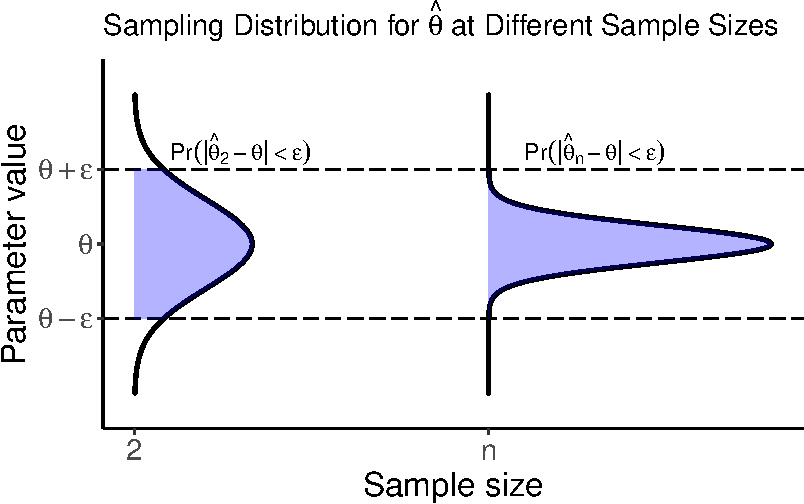
\includegraphics[keepaspectratio]{consistency_files/figure-pdf/unnamed-chunk-1-1.pdf}}

The idea here is that as our sample size gets large (as we move to the
right on the x-axis), consistency tells us something about the entire
\emph{distribution} of our estimator being within some boundary.
Asymptotic unbiasedness, on the other hand, only tells us about whether
the center of our distribution (a single point!) lies where it
``should'' (at the truth).

Why do we care about consistency? Because we care about uncertainty! It
would be really unfortunate if, in collecting more and more data, we
didn't get any more certain about the true parameter we're trying to
estimate. Intuitively, we want to be \emph{more confident} (less
uncertain) in our estimators when we have larger sample sizes. This is
exactly what consistency is concerned with. How do we prove whether or
not an estimator is consistent? (Typically) Chebyshev's Inequality,
which we state and prove below.

\section{Learning Objectives}\label{learning-objectives-4}

By the end of this chapter, you should be able to\ldots{}

\begin{itemize}
\tightlist
\item
  Distinguish between finite sample properties and asymptotic properties
  of estimators
\item
  Prove (using Chebyshev's inequality) whether or not an estimator is
  consistent
\end{itemize}

\section{Concept Questions}\label{concept-questions-4}

\begin{enumerate}
\def\labelenumi{\arabic{enumi}.}
\item
  What is the distinction between a fixed sample property and an
  asymptotic property of an estimator?
\item
  Describe, in your own words, what it means for an estimator to be
  consistent.
\item
  How can we use Chebyshev's inequality to show that an estimator is
  consistent?
\item
  Which of the estimation techniques we've seen so far yield consistent
  estimators?
\end{enumerate}

\section{Definitions}\label{definitions-4}

You are expected to know the following definitions:

\textbf{Asymptotically Unbiased}

An estimator \(\hat{\theta} = g(X_1, \dots, X_n)\) is an
\emph{asymptotically} unbiased estimator for \(\theta\) if
\(\underset{n \to \infty}{\text{lim}} E[\hat{\theta}] = \theta\).

\textbf{Consistent}

An estimator \(\hat{\theta}_n = h(X_1, \dots, X_n)\) is consistent for
\(\theta\) if it converges in probability to \(\theta\). That is, for
all \(\epsilon > 0\),

\[
\underset{n \to \infty}{\text{lim}} \Pr(| \hat{\theta}_n - \theta | < \epsilon) = 1
\]

Note that we write our estimator with a subscript \(n\) here to clarify
that our estimator depends on our sample size. There is an alternative
\(\epsilon-\delta\) definition of consistency, but we won't focus on it
for this course.

\textbf{Weak Law of Large Numbers}

For independent and identically distributed random variables
\(X_1, \dots, X_n\) with finite expectation \(\mu < \infty\),

\[
\underset{n \to \infty}{\text{lim}} \Pr(| \overline{X} - \mu | < \epsilon) = 1
\]

Alternatively, we can write that as \(n \to \infty\),
\(\overline{X} \overset{p}{\to} \mu\), where ``\(\overset{p}{\to}\)''
denotes convergence in probability.

\section{Theorems}\label{theorems-4}

\textbf{Chebyshev's Inequality}

Let \(W\) be a random variable with mean \(\mu\) and variance
\(\sigma^2\). Then for any \(\epsilon > 0\),

\[
\Pr(|W - \mu| < \epsilon) \geq 1 - \frac{\sigma^2}{\epsilon^2},
\]

or, equivalently,

\[
\Pr(|W - \mu| \geq \epsilon) \leq \frac{\sigma^2}{\epsilon^2}.
\]

Proof.

Let \(\epsilon > 0\). Then

\begin{align*}
\sigma^2 & = \text{Var}(W) \\
& = \int_{-\infty}^\infty (w-\mu)^2 f_W(w)dw \\
& = \int_{-\infty}^{\mu - \epsilon} (w-\mu)^2 f_W(w)dw + \int_{\mu - \epsilon}^{\mu + \epsilon} (w-\mu)^2 f_W(w)dw + \int_{\mu + \epsilon}^\infty (w-\mu)^2 f_W(w)dw \\
& \ge \int_{-\infty}^{\mu - \epsilon} (w-\mu)^2 f_W(w)dw + 0  + \int_{\mu + \epsilon}^\infty (w-\mu)^2 f_W(w)dw \\
&= \int_{|w-\mu|\ge \epsilon} (w-\mu)^2 f_W(w)dw \\
& \ge \int_{|w-\mu|\ge \epsilon} \epsilon^2 f_W(w)dw \\
& = \epsilon^2 \int_{|w-\mu|\ge \epsilon} f_W(w)dw\\
& = \epsilon^2 P(|W-\mu| \ge \epsilon)
\end{align*}

and rearranging yields

\begin{align*}
\sigma^2 & \geq \epsilon^2 P(|W-\mu| \ge \epsilon) \\
P(|W-\mu| \geq \epsilon) & \leq \frac{\sigma^2}{\epsilon^2}
\end{align*}

as desired.

\textbf{Corollary 1:} If \(\hat{\theta}_n\) is an unbiased estimator for
\(\theta\) and
\(\underset{n \to \infty}{\text{lim}} Var(\hat{\theta}_n) = 0\), then
\(\hat{\theta}_n\) is consistent for \(\theta\). (You'll prove this
corollary on a problem set!)

\textbf{Corollary 2:} If \(\hat{\theta}_n\) is an asymptotically
unbiased estimator for \(\theta\) and
\(\underset{n \to \infty}{\text{lim}} Var(\hat{\theta}_n) = 0\), then
\(\hat{\theta}_n\) is consistent for \(\theta\).

Note that the second corollary is a bit stronger than the first one, in
that the first corollary actually \emph{implies} the second. If an
estimator is unbiased, then it is certainly asymptotically unbiased as
well.

\section{Worked Examples}\label{worked-examples-4}

\textbf{Problem 1:} Suppose
\(X_1, \dots, X_n \overset{iid}{\sim} N(\mu, \sigma^2)\). Show that the
MLE for \(\sigma^2\) is \emph{asymptotically} unbiased.

Solution:

The MLE for \(\sigma^2\) is given by
\(\frac{1}{n} \sum_{i = 1}^n (X_i - \overline{X})^2\) (see the MLE
section of the course notes, worked example problem 2), and has
expectation \(\left( \frac{n-1}{n} \right)\sigma^2\) (see the Properties
section of the course notes, worked example problem 6). To show that
this estimator is asymptotically unbiased, note that we have

\begin{align*}
    \underset{n\to \infty}{\text{lim}} E[\hat{\sigma^2}_{MLE}] & = \underset{n\to \infty}{\text{lim}} \left( \frac{n-1}{n} \right) \sigma^2 \\
    & = \left( 1 \right) \sigma^2 \\
    & = \sigma^2
\end{align*}

and therefore, the MLE for \(\sigma^2\) is asymptotically unbiased.

\textbf{Problem 2:} Suppose
\(Y_1, \dots, Y_n \overset{iid}{\sim} Uniform(0, \theta)\), and recall
that \(\hat{\theta}_{MLE} = Y_{(n)}\) with
\(f_{Y_{(n)}}(y \mid \theta) = \frac{n}{\theta^n} y^{n-1}\),
\(0 \leq y \leq \theta\). Prove that \(\hat{\theta}_{MLE}\) is a
consistent estimator for \(\theta\).

Solution:

To prove that \(\hat{\theta}_{MLE}\) is consistent, we must first show
that \(\hat{\theta}_{MLE}\) is (either) unbiased or asymptotically
unbiased, and then we must show that the variance of
\(\hat{\theta}_{MLE}\) tends to zero as \(n \to \infty\). To begin, note
that

\begin{align*}
    E\left[\hat{\theta}_{MLE}\right] & = \int_{0}^\theta y f_{Y_{(n)}} (y \mid \theta) dy \\
    & = \int_{0}^\theta y \left( \frac{n}{\theta^n} y^{n-1} \right) dy \\
    & = \frac{n}{\theta^n} \int_0^\theta y^n dy \\
    & = \frac{n}{\theta^n} \left( \frac{y^{n + 1}}{n + 1} \bigg|_0^\theta \right) \\
    & = \frac{n}{\theta^n} \left( \frac{\theta^{n + 1}}{n + 1} \right) \\
    & = \left( \frac{n}{n + 1} \right) \theta
\end{align*}

and so \(\hat{\theta}_{MLE}\) is biased. It is, however, asymptotically
\emph{unbiased}. Note that
\(\left( \frac{n}{n + 1} \right) \overset{n \to \infty}{\to} 1\), and
therefore
\(E\left[\hat{\theta}_{MLE}\right] \overset{n \to \infty}{\to} \theta\).

All that's left is to show that
\(Var\left[\hat{\theta}_{MLE}\right] \overset{n \to \infty}{\to} 0\). We
can write

\begin{align*}
        E\left[Y_{(n)}^2\right] & = \int_0^\theta y^2 \frac{ny^{n-1}}{\theta^n} dy \\
        & = \frac{n}{\theta^n} \int_0^\theta y^{n + 1} dy \\
        & = \frac{n}{\theta^n} \left( \frac{y^{n + 2}}{n + 2} \bigg|_0^\theta \right) \\
        & = \frac{n}{\theta^n} \left( \frac{\theta^{n + 2}}{n + 2}\right) \\
        & = \left( \frac{n}{n + 2} \right) \theta^2
    \end{align*}

and therefore

\begin{align*}
    \underset{n \to \infty}{\text{lim}} Var\left[\hat{\theta}_{MLE}\right] & = \underset{n \to \infty}{\text{lim}} \left[ E\left[Y_{(n)}^2\right] - E\left[Y_{(n)}\right]^2 \right]\\
    & = \underset{n \to \infty}{\text{lim}} \left[ \left( \frac{n}{n + 2} \right) \theta^2 - \left( \frac{n}{n + 1} \right)^2 \theta^2 \right] \\
    & = \theta^2 \underset{n \to \infty}{\text{lim}} \left[ \left( \frac{n}{n + 2} \right)  - \left( \frac{n}{n + 1} \right)^2\right] \\
    & = \theta^2 \underset{n \to \infty}{\text{lim}} \left[  \frac{n}{n + 2}   - \frac{n^2}{(n + 1)^2} \right] \\
    & = \theta^2 \underset{n \to \infty}{\text{lim}} \left[  \frac{n(n + 1)^2 - n^2 (n + 2)}{(n + 2)(n + 1)^2} \right] \\
    & = \theta^2 \underset{n \to \infty}{\text{lim}} \left[  \frac{n(n^2 + 2n + 1) - n^3 -2n^2}{(n + 2)(n^2 + 2n + 1)} \right] \\
    & = \theta^2 \underset{n \to \infty}{\text{lim}} \left[  \frac{n^3 + 2n^2 + n - n^3 -2n^2}{n^3 + 2n^2 + 2n^2 + 5n + 2} \right] \\
    & = \theta^2 \underset{n \to \infty}{\text{lim}} \left[  \frac{n}{n^3 + 4n^2  + 5n + 2} \right] \\
    & = 0
\end{align*}

where the last term goes to zero because \(\frac{n}{n^3} \to 0\) as
\(n \to \infty\). Therefore, \(\hat{\theta}_{MLE}\) is a consistent
estimator for \(\theta\).

\bookmarksetup{startatroot}

\chapter{Asymptotics \& the Central Limit
Theorem}\label{asymptotics-the-central-limit-theorem}

Asymptotic unbiasedness and consistency allow us to assess the behavior
of estimators when sample sizes get large. Thus far, however, we've only
discussed what happens to \emph{point estimates} as \(n\) goes to
infinity. Point estimates are great, but they don't tell the whole
story. In order to truly quantify uncertainty (which is arguably one of
the main goals of statistics, if not \emph{the} main goal), we need to
be able to estimate a range of plausible values for our estimators: we
need to be able to construct confidence intervals. This is made possible
primarily by asymptotic normality, the Central Limit Theorem, and
properties of the normal distribution.

\subsection*{Confidence Intervals}\label{confidence-intervals}

Confidence intervals are one of the most difficult concepts for a
budding statistician to grasp, because they don't have the intuitive,
probabilistic definition we often want them to have (aka the probability
that the truth lies within the interval). As with Frequentist statistics
more generally, the definition of a confidence interval relies on the
concept of \emph{repeated sampling} from a population.

A confidence interval either contains the true parameter, or it does
not. There is no probability involved in that statement. Probability
comes into play when considering that, under repeated sampling, if we
construct confidence intervals each time we take a new sample and
construct an estimator, a given percentage \emph{of those intervals}
will contain the true parameter.

\subsubsection*{Confidence Intervals - The
CLT}\label{confidence-intervals---the-clt}

The primary way that we construct confidence intervals is by
``rearranging'' the CLT so that a quantity's asymptotic distribution
does not depend on the data nor the parameter of interest. This process
is sometimes called establishing an \emph{approximate pivotal quantity}.

As an example, consider an iid random sample \(X_1, \dots, X_n\) where
\(E[X_i] = \mu\) and \(Var[X_i] = \sigma^2\), where \(\sigma^2\) is
known. The CLT tells us that

\[
\sqrt{n}(\bar{X} - \mu) \overset{d}{\to} N(0, \sigma^2).
\]

We can use this to construct a confidence interval for \(\mu\). By
Slutsky's theorem we can write

\[
\frac{\bar{X} - \mu}{\sigma/\sqrt{n}} \overset{d}{\to} N(0, 1).
\]

and note now that we \emph{know} the asymptotic distribution for the
(pivotal) quantity on the left, and can therefore use the
\emph{quantiles} of this distribution to construct confidence intervals.
For a standard normal distribution (as is the case here) we can note
that 95\% of the distribution is contained within 1.96 standard
deviations of the mean, and therefore

\[
\Pr\left(-1.96 \leq \frac{\bar{X} - \mu}{\sigma/\sqrt{n}} \leq 1.96\right) = 0.95
\]

We can rearrange the probability statement on the left hand side to get

\[
\Pr\left(\bar{X}-1.96 \sigma/\sqrt{n} \leq \mu \leq \bar{X} + 1.96\sigma/\sqrt{n}\right) = 0.95
\]

and therefore, our 95\% confidence interval for \(\mu\) is given by
\(\left( \bar{X}-1.96 \sigma/\sqrt{n}, \bar{X}+1.96 \sigma/\sqrt{n} \right)\).

\subsubsection*{Confidence Intervals -
``Exact''}\label{confidence-intervals---exact}

A second way that we construct confidence intervals is through a
concrete distributional assumption, and known quantiles of those
distributions. Note that the confidence interval constructed above
involves the Central Limit Theorem, and \emph{no} \emph{finite sample}
distributional assumption. All we assume are that the data are iid
observations with finite means and variances. The ``distribution'' only
comes into play as our sample size gets large.

When sample sizes \emph{aren't} large, applying the CLT might not make a
whole lot of sense. In these scenarios, it can be useful to use an
alternative confidence interval construction, aided by assuming a
specific distribution for our random variables. In some scenarios these
assumptions may make more sense than others: in short, we're
\emph{always} making some sort of assumption, regardless of what we do.
It's part of our job as statisticians to ensure that the assumptions we
make, make sense for the application we're working with!

One example of a commonly used ``exact'' confidence interval is the
\href{https://en.wikipedia.org/wiki/Binomial_proportion_confidence_interval\#Clopper\%E2\%80\%93Pearson_interval}{Clopper-Pearson}
interval for a binomial proportion. Consider an iid random sample
\(X_1, \dots, X_n\), where \(\sum_{i = 1}^n X_i \sim Binomial(n, p)\).
Intuitively, the interval is constructed by the following steps:

\begin{enumerate}
\def\labelenumi{\arabic{enumi}.}
\item
  Find the \emph{largest} p such that \(\Pr(X \leq k) \geq \alpha/2\),
  where \(k\) is the observed number of successes. Call this largest
  value \(p_U\).
\item
  Find the \emph{smallest} p such that \(\Pr(X \geq k) \geq \alpha/2\),
  where \(k\) is again the observed number of successes. Call this
  smallest value \(p_L\).
\item
  Define the \(100(1 -\alpha)\)\% confidence interval for \(p\) to be
  \((p_U, p_L)\).
\end{enumerate}

This construction process allows us to determine all possible values of
\(p\) that are compatible with our observed number of successes (which
is exactly what a confidence interval should do).

In more math-y terms, We can show that if
\(\sum_{i = 1}^n X_i \sim Binomial(n, p)\), then
\(\Pr(\sum_{i = 1}^n X_i \geq x) = \Pr(Y \leq p)\), where
\(Y \sim Beta(\sum_{i = 1}^n x_i, n - \sum_{i = 1}^n x_i + 1)\). The
point of doing this is that we can rewrite our probability statements
(involved in our confidence interval construction) in terms of a random
variable that \emph{does not depend} on \(p\). We can then compute the
Clopper-Pearson interval for \(p\) as

\[
\Phi_{\frac{\alpha}{2}; \sum_{i = 1}^n x_i, n - \sum_{i = 1}^n x_i + 1} < p < \Phi_{1 - \frac{\alpha}{2}; \sum_{i = 1}^n x_i + 1, n - \sum_{i = 1}^n x_i}
\]

where \(\Phi_{a; v, w}\) is the \(a\)th quantile from a Beta
distribution with shape parameters \(v\) and \(w\). Alternatively, you
can even write the Clopper-Pearson in terms of quantiles of the
\(F\)-distribution, but the Beta format is enough to emphasize the main
point: If we can determine the distribution of some function of our data
and unknown parameter, and manipulate that distribution enough so that
it depends on neither the data nor unknown parameter, we can use
quantiles and probability statements to construct confidence intervals.

\subsection*{Convergence}\label{convergence}

If an estimator \(\hat{\theta}_n\) is a consistent estimator for
\(\theta\), we also say that \(\hat{\theta}_n\) converges in probability
to \(\theta\) (i.e., \(\hat{\theta}_n \overset{p}{\to} \theta\)). There
are three different types of convergence: almost sure convergence,
convergence in probability, and convergence in distribution (in order
from ``strongest'' to ``weakest''). The main two that we'll care about
for this course are convergence in probability and convergence in
distribution. For our purposes, it will \emph{mostly} suffice to know
that (1) convergence in probability \emph{implies} convergence in
distribution, (2) the Central Limit Theorem, delta-method, and Slutsky's
Theorem are tools we can use to determine (and manipulate) asymptotic
distributions of random variables, and (3) the Continuous Mapping
Theorem (defined below). That being said, an attempt at an intuitive
explanation of these three types of convergence is provided below, in
the context of sequences of random variables.

\subsubsection{Convergence Almost
Surely}\label{convergence-almost-surely}

Convergence almost surely is the strongest of the three types of
convergence. A sequence of random variables \(X_1, \dots, X_n\)
convergences almost surely (also called convergence almost everywhere)
if

\[
\Pr(\lim_{n \to \infty} X_n = X) = 1
\]

In my opinion, one of the most intuitive explanations for convergence
almost surely (and convergence in probability, comparatively) is given
in the top answer to
\href{https://stats.stackexchange.com/questions/2230/convergence-in-probability-vs-almost-sure-convergence}{this}
StackExchange post. Convergence almost surely says that \(X_n\)
\emph{will} be equal to \(X\) at some point, for finite \(n\).

\subsubsection{Convergence in
Probability}\label{convergence-in-probability}

Surprise! You already know this one, if you made it through the
Consistency chapter. The concept of convergence in probability applies
to sequences of random variables in addition to estimators. A sequence
of random variables \(X_1, \dots, X_n\) converges in probability towards
the random variable \(X\) if for all \(\epsilon > 0\)

\[
\lim_{n \to \infty} \Pr(|X_n - X | > \epsilon) = 0
\]

Note that this equivalent to saying that
\(\lim_{n \to \infty} \Pr(|X_n - X | \leq \epsilon) = 1\), which looks a
bit more like what we saw last chapter. Convergence in probability says
that \(X_n\) will equal \(X\) \emph{with a very high probability} as
\(n\) gets large, though there will always be some small (shrinking with
\(n\)) chance that they aren't equal.

\subsubsection{Convergence in
Distribution}\label{convergence-in-distribution}

A sequence of random variables \(X_1, \dots, X_n\) with CDFs
\(F_1, \dots, F_n\) converges in distribution (also called ``weak''
convergence, or convergence in ``law'') if

\[
\lim_{n \to \infty} F_n(x) = F(x)
\]for every number \(x\) at which \(F\) is continuous. Note that
\emph{unlike} convergence almost surely and convergence in probability,
our sequence of variables isn't ``shrinking'' in quite the same way,
with this type of convergence. Rather, our sequence is better and better
approximating an \emph{entire distribution}, rather than focusing in on
a single point. A visual representation of convergence in distribution
is provided below, where \(F_n(x)\) is the black sequence of lines, and
the red line is \(F(x)\).

\subsection*{Asymptotic Properties of
MLEs}\label{asymptotic-properties-of-mles}

In addition to the nice intuition behind maximum likelihood estimation
(finding the parameters that make our data the most likely to have
occurred), most* MLEs also have incredibly convenient asymptotic
properties, including:

\begin{itemize}
\item
  Asymptotic unbiasedness
\item
  Consistency
\item
  Asymptotic normality
\item
  Asymptotic efficiency
\end{itemize}

The definitions of the latter two properties are included below (and the
former in the previous chapters).

*the MLEs that do not have all of these properties are the ones that
don't have certain ``regularity conditions.'' For the MLEs we consider
in this class, these are the MLEs that are on the boundary of the
support of the pdf (such as the maximum or minimum order statistic).

\section{Learning Objectives}\label{learning-objectives-5}

By the end of this chapter, you should be able to\ldots{}

\begin{itemize}
\item
  Explain the usefulness of the Central Limit Theorem for Frequentist
  statistical theory
\item
  Manipulate asymptotic distributions to remove their dependence on
  unknown parameters using the delta-method and Slutsky's theorem

  \begin{itemize}
  \tightlist
  \item
    \ldots and explain why such manipulation is important for confidence
    interval construction
  \end{itemize}
\item
  Derive confidence intervals for unknown parameters based on asymptotic
  or exact distributions
\end{itemize}

\section{Concept Questions}\label{concept-questions-5}

\begin{enumerate}
\def\labelenumi{\arabic{enumi}.}
\item
  What feature of a confidence interval tells us about the precision of
  our estimator?
\item
  Why is ``removing'' unknown parameters from the asymptotic
  distribution of our estimators important when constructing confidence
  intervals?
\end{enumerate}

\section{Definitions}\label{definitions-5}

\textbf{Asymptotic Normality}

An estimator \(\hat{\theta}_n\) is asymptotically normal if
\(\hat{\theta}_n\) converges in distribution to a normally distributed
random variable.

\textbf{Asymptotic Efficiency}

An estimator \(\hat{\theta}_n\) is asymptotically efficient if it's
asymptotic variance attains the C-R Lower Bound. Note that this is the
C-R Lower Bound for a \emph{single} observation, and therefore the
asymptotic distribution of an MLE looks something like this:

\[
\sqrt{n} (\hat{\theta}_n - \theta) \overset{d}{\to} N\left( 0, \frac{1}{I_1(\theta)}\right)
\]

\textbf{Confidence Interval}

A 100(1 - \(\alpha\))\% confidence interval for a parameter \(\theta\)
is given by \((a, b)\), where
\(\Pr(a \leq \theta \leq b) = 1 - \alpha\).

\section{Theorems}\label{theorems-5}

\textbf{Central Limit Theorem (CLT)}

For iid random variables \(X_1, \dots, X_n\) with mean \(\mu\) and
variance \(\sigma^2\),

\[
\sqrt{n} (\bar{X_n} - \mu) \overset{d}{\to} N(0, \sigma^2)
\]

where ``\(\overset{d}{\to}\)'' denotes convergence in distribution.

Proof.

Note that this proof is not completely rigorous, in that we will use the
following theorem (without proof) in order to prove the CLT:

Theorem: Let \(W_1, \dots, W_n\) be a sequence of random variables with
MGF of the sequence \(W_n\) given by \(M_{W_n}(t)\). Also, let \(V\)
denote another random variable with MGF \(M_V(t)\). Then if
\(\underset{n \to \infty}{\text{lim}} M_{W_n}(t) = M_V(t)\), for all
values of \(t\) in some interval around \(t = 0\), then the sequence
\(W_1, \dots, W_n\) converges in distribution to \(V\).

Suppose \(X_1, \dots, X_n\) with mean \(\mu\) and variance \(\sigma^2\),
and let \(Y_i = (X_i - \mu)/\sigma\). Then \(E[Y_i] = 0\), and
\(Var[Y_i] = 1\) since

\[
E[Y_i] = E \left[ (X_i - \mu)/\sigma\right] = \frac{1}{\sigma} (E[X_i] - \mu) = \frac{1}{\sigma} (\mu - \mu) = 0
\]

and

\[
Var[Y_i] = Var\left[ (X_i - \mu)/\sigma\right] = \frac{1}{\sigma^2} Var[X_i - \mu] = \frac{1}{\sigma^2} Var[X_i] = \frac{\sigma^2}{\sigma^2} = 1
\]

Further, let

\[
Z_n = \frac{\sqrt{n}(\bar{X} - \mu)}{\sigma} = \frac{1}{\sqrt{n}} \sum_{i = 1}^n Y_i
\]

where the last two terms are equal since

\begin{align*}
    \frac{1}{\sqrt{n}} \sum_{i = 1}^n Y_i & = \frac{1}{\sqrt{n}} \sum_{i = 1}^n \left( \frac{X_i - \mu}{\sigma}\right)\\
    & = \frac{1}{\sigma\sqrt{n}} \sum_{i = 1}^n (X_i - \mu) \\
    & = \frac{1}{\sigma\sqrt{n}}  (n\bar{X} - n\mu) \\
    & = \frac{\sqrt{n}(\bar{X} - \mu)}{\sigma}
\end{align*}

We'll show that \(Z_n \overset{d}{\to} N(0,1)\) by showing that the MGF
of \(Z_n\) converges to the MGF of a standard normal distribution. Let
\(M_Y(t)\) denote the MGF of each \(Y_i\). Then the MGF of
\(\sum_{i = 1}^n Y_i\) is given by

\[
E[e^{t\sum_{i = 1}^n Y_i}] = E[e^{tY_1}e^{tY_2} \dots e^{tY_n}] = E[e^{tY_1}]E[e^{tY_2}] \dots E[e^{tY_n}] = M_Y(t)^n
\]

and the MGF of \(Z_n\) is

\[
M_{Z_n}(t) = E[e^{tZ_n}] = E[e^{t\frac{1}{\sqrt{n}}\sum_{i = 1}^n Y_i}] = M_Y\left(\frac{t}{\sqrt{n}}\right)^n
\]

Now note that the Taylor expansion of the function \(e^{tY}\) about
\(0\) is given by

\[
e^{tY} = 1 + tY + \frac{t^2Y^2}{2!} + \frac{t^3Y^3}{3!} + \dots
\]

Taking the expectation of both sides, we obtain

\[
E[e^{tY}] = 1 + tE[Y] + \frac{t^2E[Y^2]}{2!} + \frac{t^3E[Y^3]}{3!} + \dots
\]

and note now that the left hand side is the MGF for \(Y\). Recalling
that \(E[Y] = 0\) and \(Var[Y] = 1\), we have

\[
E[e^{tY}] = 1  + \frac{t^2}{2!} + \frac{t^3E[Y^3]}{3!} + \dots
\]

And therefore

\[
E[e^{tZ_n}] = \left[1  + \frac{t^2}{2n} + \frac{t^3E[Y^3]}{3!n^{3/2}} + \dots \right]^n
\]

We'll now make use of a theorem regarding sequences of real numbers
(without proof): Let \(a_n\) and \(c_n\) be sequences of real numbers
such that \(a_n \overset{n \to \infty}{\to} 0\) and
\(c_na_n^2 \overset{n \to \infty}{\to} 0\). Then if
\(a_nc_n \overset{n \to \infty}{\to} b\),
\((1 + a_n)^{c_n} \overset{n \to \infty}{\to} e^b\).

Let \(a_n = \frac{t^2}{2n} + \frac{t^3E[Y^3]}{3!n^{3/2}} + \dots\) and
\(c_n = n\). Note that both \(a_n \overset{n \to \infty}{\to} 0\) and
\(c_na_n^2 \overset{n \to \infty}{\to} 0\). Then

\[
\underset{n \to \infty}{\text{lim}} a_n c_n = \underset{n \to \infty}{\text{lim}} \left[ \frac{t^2}{2} + \frac{t^3E[Y^3]}{3!n^{1/2}} + \dots\right] = \frac{t^2}{2}
\]

and therefore

\[
M_{Z_n}(t) = (1 + a_n)^{c_n} \overset{n \to \infty}{\to} e^{t^2/2}
\]

where we note that the right hand side is the MGF of a standard normal
distribution. Then finally, we have proved that

\[
\sqrt{n}(\bar{X} - \mu) \overset{d}{\to} N(0, \sigma^2)
\]

as desired.

\textbf{Continuous Mapping Theorem}

If \(X_n \overset{p}{\to} X\), and \(g\) is a continuous function, then
\(g(X_n) \overset{p}{\to} g(X)\). Similarly for convergence almost
surely and convergence in distribution.

Proof.

Left to the reader, but also on
\href{https://en.wikipedia.org/wiki/Continuous_mapping_theorem\#Proof}{Wikipedia}.

\textbf{Slutsky's Theorem}

If \(g(X, Y)\) is a jointly continuous function at every point
\((X, a)\) for some fixed \(a\), and if \(X_n \overset{d}{\to} X\) and
\(Y_n \overset{p}{\to} a\), then
\(g(X_n, Y_n) \overset{d}{\to} g(X, a)\).

Proof.

Beyond the scope of the course, unfortunately, but here's a
\href{https://en.wikipedia.org/wiki/Slutsky\%27s_theorem\#Proof}{link}
to the Wikipedia page if you want to go down that rabbit hole in your
spare time.

\textbf{Delta-method}

Let \(\sqrt{n} (Y - \mu) \overset{d}{\to} N(0, \sigma^2)\). If \(g(Y)\)
is differentiable at \(\mu\) and \(g'(\mu) \neq 0\), then

\[
\sqrt{n} \left( g(Y) - g(\mu)\right) \overset{d}{\to} N(0, [g'(\mu)]^2 \sigma^2)
\]

Proof.

Since \(g\) is differentiable at \(\mu\), it's first-order Taylor
expansion is given by

\[
g(Y) = g(\mu) + (Y - \mu)g'(\mu) + O(| Y - \mu |^2)
\]

where \(O(f(x))\), referred to as ``Big O,'' describes the limiting
behavior of the function \(f(x)\). In this case, we use it to note that
every term in the Taylor expansion after the first derivative evaluated
at \(\mu\) is growing no faster than \(|Y - \mu|^2\) as
\(n \to \infty\).

Rearranging, note that

\[
g(Y) - g(\mu) =  (Y - \mu)g'(\mu) + O(| Y - \mu |^2)
\]

and so

\begin{align*}
    \sqrt{n}\left( g(Y) - g(\mu) \right) = \sqrt{n}(Y - \mu) g'(\mu) + O(\sqrt{n} |Y - \mu|^2)
\end{align*}

Then note that \(\sqrt{n}(Y - \mu) \overset{d}{\to} N(0, \sigma^2)\),
\(g'(\mu) \overset{p}{\to} g'(\mu)\) since it's just a constant, and
\(O(\sqrt{n} |Y - \mu|^2) \overset{p}{\to} 0\). To see the latter, note
that \(1/\sqrt{n} \to 0\), and so by Slutksy's

\begin{align*}
\frac{1}{\sqrt{n}} \sqrt{n}(Y - \mu) & \overset{d}{\to} N(0, \sigma^2) \times 0 \\
 Y - \mu & \overset{d}{\to} 0
\end{align*} and if a random variable (in this case \(Y - \mu\))
converges in distribution to a constant, that implies that it converges
in probability to that same constant (see Wikipedia
\href{https://en.wikipedia.org/wiki/Proofs_of_convergence_of_random_variables\#propB1}{here}).
Then the CLT actually \emph{implies} consistency of \(Y\) for \(\mu\).

Note that we have just shown that not only is \(Y\) consistent for
\(\mu\), but that it converges to \(\mu\) at a \(1/\sqrt{n}\) rate, in
probability. We can write this as
\(Y - \mu = O_p\left(\frac{1}{\sqrt{n}}\right)\), and therefore

\[
\sqrt{n} | Y - \mu |^2 = \sqrt{n} \left( O_p\left( \frac{1}{\sqrt{n}}\right) \right)^2 = \sqrt{n} O_p\left( \frac{1}{n} \right) = O_p(1/\sqrt{n}) \overset{p}{\to} 0
\]

Finally, using two applications of Slutsky's theorem, we can write that

\[
\sqrt{n}(Y - \mu)g'(\mu) \overset{d}{\to} N(0, \sigma^2)g'(\mu) = \overset{d}{\to} N(0, [g'(\mu)]^2\sigma^2)
\] and

\begin{align*}
    \sqrt{n}(Y - \mu)g'(\mu) + O(\sqrt{n} |Y - \mu|^2) & \overset{d}{\to} N(0, \sigma^2)g'(\mu) + 0\\
    & \overset{d}{=} N(0, [g'(\mu)]^2\sigma^2) 
\end{align*}

and so we have shown that \[
\sqrt{n}\left( g(Y) - g(\mu) \right) \overset{d}{\to}  N(0, [g'(\mu)]^2\sigma^2)
\] as desired.

\textbf{Asymptotic Normality \& Efficiency of MLEs}

Suppose that for iid observations \(X_1, \dots, X_n\), \(\hat{\theta}\)
is the MLE for \(\theta_0\). Then we have that

\[
\sqrt{n} (\hat{\theta} - \theta_0) \overset{d}{\to} N\left(0, \frac{1}{I_1(\theta_0)}\right)
\]

\emph{Lemma.} Let \(\theta_0\) denote the true unknown value of the
parameter \(\theta\) for a density given by \(f(x \mid \theta)\). Then
for any other \(\theta\), we have that
\(E[\log f(x \mid \theta)] \leq E[\log f(x \mid \theta_0)]\).

Proof of Lemma:

To show that
\(E[\log f(x \mid \theta)] \leq E[\log f(x \mid \theta_0)]\), we can
equivalently show that
\(E[\log f(x \mid \theta)] - E[\log f(x \mid \theta_0)] \leq 0\). Note
that we can write

\begin{align*}
    E[\log f(x \mid \theta)] - E[\log f(x \mid \theta_0)] & = E[\log f(x \mid \theta) - \log f(x \mid \theta_0)] \quad \text{(linearity of expectation)} \\
    & = E\left[ \log \frac{ f(x \mid \theta)}{f(x \mid \theta_0)} \right] \quad \text{(log rules)} \\
    & \leq E\left[ \frac{ f(x \mid \theta)}{f(x \mid \theta_0)} - 1 \right] \quad \text{(log $t \leq t - 1$)} \\
    & = \int \left( \frac{ f(x \mid \theta)}{f(x \mid \theta_0)} - 1 \right)  f(x \mid \theta_0) dx \\
    & = \int \left( \frac{ f(x \mid \theta)}{f(x \mid \theta_0)} - \frac{ f(x \mid \theta_0)}{f(x \mid \theta_0)} \right)  f(x \mid \theta_0) dx \\
    & = \int f(x \mid \theta) - f(x \mid \theta_0) dx \\
    & = \int f(x \mid \theta) dx - f(x \mid \theta_0) dx \\
    & = 1 - 1 \quad \text{(pdfs integrate to 1)} \\
    & = 0
\end{align*}

as desired.

Proof of Theorem:

Just as in the theorem statement, suppose \(\hat{\theta}\) is the MLE
for \(\theta_0\), where we have iid observations \(X_1, \dots, X_n\)
with some density function given by \(f(x_i \mid \theta)\). Let
\(\log L(\theta)\) denote the \textit{expectation} of the log
likelihood, \(E[\log f(\textbf{x} \mid \theta)]\), and let
\(L_n(\theta)\) denote the log likelihood divided by the sample size,
\(L_n(\theta) = \frac{1}{n}\sum_{i = 1}^n \log f(x_i \mid \theta)\).
Note that by definition of an MLE, \(L_n'(\hat{\theta}) = 0\) (the first
derivative of \(L_n(\theta)\) evaluated at \(\hat{\theta}\) is equal to
zero).

Recall that the Mean Value Theorem (MVT) states that

\[
\frac{f(a) - f(b)}{a - b} = f'(c), \quad c \in [a,b],
\]

Let \(f(\theta) = L_n'(\theta)\), \(a = \hat{\theta}\), and
\(b = \theta_0\). Then the MVT gives us that

\begin{align*}
    \frac{L_n'(\hat{\theta}) - L_n'(\theta_0)}{\hat{\theta} - \theta_0} &= L_n''(\theta) \\
    L_n'(\hat{\theta}) - L_n'(\theta_0) & = L_n''(\theta) (\hat{\theta} - \theta_0) \\
     L_n'(\hat{\theta}) & = L_n'(\theta_0) + L_n''(\theta) (\hat{\theta} - \theta_0) \\
    0 & = L_n'(\theta_0) + L_n''(\theta) (\hat{\theta} - \theta_0) \quad \text{(by definition of MLE)}
\end{align*}

for some \(\theta \in [\hat{\theta}, \theta_0]\). Rearranging and
multiplying both sides by \(\sqrt{n}\) yields

\begin{align*}
    0 & = L_n'(\theta_0) + L_n''(\theta) (\hat{\theta} - \theta_0) \\
    - L_n'(\theta_0) & = L_n''(\theta) (\hat{\theta} - \theta_0) \\
    -\frac{L_n'(\theta_0)}{L_n''(\theta)} & = \hat{\theta} - \theta_0 \\
    -\frac{\sqrt{n}L_n'(\theta_0)}{L_n''(\theta)} & = \sqrt{n}(\hat{\theta} - \theta_0)
\end{align*}

Now note that by the previous lemma, \(E[\log f(x \mid \theta)]\) is
maximized at \(\theta_0\), and therefore \(L'(\theta_0) = 0\). Then we
can write

\begin{align*}
    \sqrt{n}L_n'(\theta_0) & = \sqrt{n}(L_n'(\theta_0) - 0) \\
    & = \sqrt{n} \left( L_n'(\theta_0) - L'(\theta_0)\right) \\
    & = \sqrt{n} \left( \frac{1}{n} \sum_{i = 1}^n \frac{\partial}{\partial \theta_0} \log f(x_i \mid \theta_0) - E\left[ \frac{\partial}{\partial \theta_0} \log f(x_i \mid \theta_0)\right] \right) \\
    & \overset{d}{\to} N \left( 0, \text{Var}\left( \frac{\partial}{\partial \theta_0} \log f(x_i \mid \theta_0) \right) \right), \quad \text{(Central Limit Theorem!)}
\end{align*}

And by definition of variance, we have that

\begin{align*}
    \text{Var}\left( \frac{\partial}{\partial \theta_0} \log f(x_i \mid \theta_0) \right) & = E \left[ \left( \frac{\partial}{\partial \theta_0} \log f(x_i \mid \theta_0) \right)^2 \right] - E \left[ \left( \frac{\partial}{\partial \theta_0} \log f(x_i \mid \theta_0) \right)\right]^2 \\
    & = I_1(\theta_0) - (L'(\theta_0))^2 \quad \text{(definition of information)} \\
    & = I_1(\theta_0)
\end{align*}

and so we have that

\[
\sqrt{n} L_n'(\theta_0) \overset{d}{\to} N(0, I_1(\theta_0))
\]

Now note that

\begin{align*}
    L_n''(\theta) = \frac{1}{n} \sum_{i = 1}^n \left( \frac{\partial^2}{\partial \theta^2} \log f(x_i \mid \theta) \right)
\end{align*}

and by the WLLN,
\(-L_n''(\theta) \overset{p}{\to} -E\left[ \frac{\partial^2}{\partial \theta^2} \log f(x_i \mid \theta) \right] = I_1(\theta_0)\),
by definition of the information matrix. Then applying Slutsky's theorem
gives us that

\begin{align*}
    \sqrt{n} (\hat{\theta} - \theta_0) & = - \frac{\sqrt{n} L_n'(\theta_0)}{L_n''(\theta)} \\
    & \overset{d}{\to} N(0, I_1(\theta_0)) \frac{1}{I_1(\theta_0)} \\
    & \overset{d}{=} N\left( 0, \frac{I_1(\theta_0)}{I_1(\theta_0)^2}\right) \\
    & \overset{d}{=} N\left( 0, \frac{1}{I_1(\theta_0)}\right)
\end{align*}

as desired.

\section{Worked Examples}\label{worked-examples-5}

\textbf{Problem 1:} Suppose
\(\sqrt{n}(Y_n - \mu) \overset{d}{\to} N(0, \sigma^2)\). Find the
asymptotic distribution of \(\sqrt{n}(Y_n^2 - \mu^2)\) when
\(\mu \neq 0\).

Solution:

We can apply the delta-method with the function \(g(x) = x^2\). Note
that \(g'(x) = 2x\), and therefore we can write

\begin{align*}
    \sqrt{n}(Y_n - \mu) & \overset{d}{\to} N(0, \sigma^2) \\
    \sqrt{n}(g(Y_n) - g(\mu)) & \overset{d}{\to} N(0, [g'(\mu)]^2\sigma^2) \\
    \sqrt{n}(Y_n^2 - \mu^2) & \overset{d}{\to} N(0, [2\mu]^2\sigma^2) \\
    \sqrt{n}(Y_n^2 - \mu^2) & \overset{d}{\to} N(0, 4 \mu^2\sigma^2)
\end{align*}

\textbf{Problem 2:} Suppose
\(X_1, \dots, X_n \overset{iid}{\sim} Bernoulli(p)\), and recall that
the MLE for \(p\) is given by
\(\hat{p}_{MLE} = \frac{1}{n} \sum_{i = 1}^n X_i\). Find the asymptotic
distribution of \(\hat{p}_{MLE}\) using the CLT and known properties of
the Bernoulli distribution (expectation and variance, for example), and
construct a 95\% confidence interval for \(p\) based on this asymptotic
distribution.

Solution:

We know that \(E[X_i] = p\) and \(Var[X_i] = p(1-p)\). Then the CLT tell
us that

\[
\sqrt{n}(\hat{p}_{MLE} - p) \overset{d}{\to} N(0, p(1-p))
\]

The WLLN gives us that \(\hat{p}_{MLE} \overset{p}{\to} p\), since
\(\hat{p}_{MLE}\) is a sample mean. We can then use the continuous
mapping theorem to show that
\(\frac{1}{\sqrt{\hat{p}_{MLE}(1-\hat{p}_{MLE})}} \overset{p}{\to} \frac{1}{\sqrt{p(1 - p)}}\).
Applying Slutsky's theorem, we then have

\[
\sqrt{n}\left(\frac{\hat{p}_{MLE} - p}{\sqrt{\hat{p}_{MLE}(1-\hat{p}_{MLE})}}\right) \overset{d}{\to} N(0, 1)
\]

and finally, (letting \(\hat{p} = \hat{p}_{MLE}\) for ease of notation)

\begin{align*}
    0.95 & = \Pr\left(-1.96 < \frac{\hat{p} - p}{\sqrt{\hat{p}(1-\hat{p})/n}}  < 1.96\right)  \\
    & = \Pr\left(-1.96\sqrt{\hat{p}(1-\hat{p})/n} < \hat{p} - p  < 1.96\sqrt{\hat{p}(1-\hat{p})/n}\right) \\
    & = \Pr\left(\hat{p} -1.96\sqrt{\hat{p}(1-\hat{p})/n} <  p  < \hat{p} + 1.96\sqrt{\hat{p}(1-\hat{p})/n}\right)
\end{align*}

\bookmarksetup{startatroot}

\chapter{Hypothesis Testing}\label{hypothesis-testing}

The goal of hypothesis testing is to make a decision between two
conflicting theories, or ``hypotheses.'' The process of hypothesis
testing involves the following steps:

\begin{enumerate}
\def\labelenumi{\arabic{enumi}.}
\item
  State the hypotheses: \(H_0\) (null hypothesis) vs \(H_1\)
  (alternative hypothesis)
\item
  Investigate: are data compatible with \(H_0\)? assuming \(H_0\) were
  true, are data extreme?
\item
  Make a decision: reject \(H_0\) or fail to reject \(H_0\)
\end{enumerate}

The first step is relatively straightforward. For the purposes of this
course, our null hypothesis will always be that some unknown parameter
we are interested in \((\theta)\) is equal to a fixed point
\((\theta_0)\). We'll consider two possible alternatives hypothesis:

\begin{itemize}
\item
  \(H_1: \theta = \theta_1\) (``simple'' alternative)
\item
  \(H_1: \theta \neq \theta_0\) (two-sided alternative)
\end{itemize}

The former is the simplest, non-trivial alternative hypothesis we can
consider, and we can prove some nice things in this setting (and hence
build intuition for hypothesis testing broadly). The latter is perhaps
more relevant, particularly in linear regression.

If you recall from introductory statistics, the latter alternative
provides the set-up we have when testing if the linear relationship
between a predictor \(X\) and outcome \(Y\) are ``statistically
significantly'' associated; we test the null hypothesis
\(H_0: \beta_1 = 0\) against the alternative, \(H_1: \beta_1 \neq 0\),
where \(E[Y \mid X] = \beta_0 + \beta_1 X\). In this example, we'd have
the unknown parameter \(\beta_1\), and the fixed point of our null
hypothesis as \(\theta_0 = 0\).

The second step of hypothesis testing is the investigation. In
determining whether the data are compatible with the null hypothesis, we
must first derive a \emph{test statistic}. Test statistics are typically
functions of (1) our estimators and (2) the distribution of our
estimator \emph{under the null hypothesis}. Intuitively, if we can
determine the distribution of our estimator under the null hypothesis,
we can then observe whether or not the data we actually have is
``extreme'' or not, given a certain threshold, \(\alpha\), for our
hypothesis test. This threshold \(\alpha\) is directly related to a
\(100(1 - \alpha)\%\) confidence interval, where anything observed
outside the confidence interval bounds is considered to lie in the
``rejection region'' (where you would thus reject the null hypothesis).

There are three classical forms of test statistics that have varying
finite-sample properties, and can be shown to be asymptotically
equivalent: the Wald test, the likelihood ratio test (LRT), and the
score test (also sometimes called the Lagrange multiplier test). Each of
these is explained in further detail below.

\subsection*{Wald Tests}\label{wald-tests}

Suppose we are interested in testing the hypotheses
\(H_0: \theta = \theta_0\) vs.~\(H_1: \theta \neq \theta_0\). The Wald
test is the hypothesis test that uses the Wald test statistic
\(\lambda_{W}\), where

\[
\lambda_W = \left( \frac{\hat{\theta}_{MLE} - \theta_0}{se(\hat{\theta}_{MLE})}\right)^2.
\]

Intuitively, the Wald test measures the difference between the estimated
value for \(\theta\) and the null value for \(\theta\), standardized by
the variation of your estimator. If this reminds you (once again) of a
z-score, it should! In linear regression, with normally distributed
standard errors, it turns out that \(\sqrt{W}\) follows a \(t\)
distribution (we'll show this on your problem set!).

Wald tests statistics are extremely straightforward to compute from the
Central Limit Theorem. The CLT states that, for iid \(X_1, \dots, X_n\)
with expectation \(\mu\) and variance \(\sigma\),

\[
\sqrt{n} (\overline{X} - \mu) \overset{d}{\to} N(0, \sigma^2).
\]

Slutsky's theorem allows us to write

\[
\left( \frac{\overline{X} - \mu}{\sigma / \sqrt{n}}\right) \overset{d}{\to} N(0,1),
\]

and note that the left-hand side is an estimator minus it's expectation,
divided by it's standard error. When \(\overline{X}\) is the MLE for
\(\mu\), this is the square root of the Wald test statistic! The final
thing to note is that the right-hand side tells us this quantity
converges in distribution to a standard normal distribution. Think about
what we've previously shown about standard normals ``squared'' to intuit
the asymptotic distribution of a Wald test statistic: a \(\chi^2_\nu\)
random variable, where the degrees of freedom \(\nu\) in this case is
one! For a single parameter restriction (i.e.~one hypothesis for one
unknown parameter), the asymptotic distribution of a Wald test statistic
will always be \(\chi^2_1\).

\subsubsection*{Wald Tests for Multiple
Hypotheses}\label{wald-tests-for-multiple-hypotheses}

Note that there is also a multivariate version of the Wald test, used to
jointly test \emph{multiple} hypotheses on multiple parameters. In this
case, we can write our null and alternative hypotheses using matrices
and vectors.

As a simple example, consider a linear regression model where we have a
single, categorical predictor with three categories. Our regression
model looks something like this:

\[
E[Y \mid X] = \beta_0 + \beta_1 X_{Cat2} + \beta_2 X_{Cat3}
\]

If we want to test if there is a significant association between \(Y\)
and \(X\), we can't look at \(\hat{\beta_1}\) and \(\hat{\beta}_2\)
separately. Rather, we need to test the joint null hypothesis
\(\beta_1 = \beta_2 = 0\), vs.~the alternative where \emph{at least one}
of our coefficients is \emph{not} equal to zero. In introductory
statistics, we did this using the \texttt{anova} function in R. In
matrix form, we can write our null and alternative hypotheses as:

\begin{itemize}
\item
  \(H_0: R \boldsymbol{\beta} = \textbf{r}\)
\item
  \(H_1: R \boldsymbol{\beta} \neq \textbf{r}\)
\end{itemize}

where \(R\) in this case is the identity matrix,
\(\boldsymbol{\beta} = (\beta_0, \beta_1)^\top\), and
\(\textbf{r} = (0,0)^\top\). The Wald test statistic in this
multi-hypothesis, multi-parameter case can then be written as

\[
(R\hat{\boldsymbol{\theta}} - \textbf{r})^\top [R (\hat{V}/n) R^\top]^{-1} (R\hat{\boldsymbol{\theta}} - \textbf{r})
\]

where \(\hat{V}\) is an estimator of the covariance matrix for
\(\hat{\boldsymbol{\theta}}\). We won't focus on multi-hypothesis,
multi-parameter tests in this course, but I \emph{do} want you to be
able to draw connections between statistical theory and things you
learned way back in your introductory statistics course, hence why this
is included in the notes.

\subsection*{Likelihood Ratio Tests}\label{likelihood-ratio-tests}

Suppose we are interested in testing the hypotheses
\(H_0: \theta = \theta_0\) vs.~\(H_1: \theta \neq \theta_0\). The
likelihood ratio test is the hypothesis test that uses the likelihood
ratio test statistic \(\lambda_{LRT}\), where

\[
\lambda_{LRT} = -2 \log\left(\frac{\underset{\theta = \theta_0}{\text{sup}} \hspace{1mm} L(\theta)}{\underset{\theta \in \Theta}{\text{sup}} \hspace{1mm} L(\theta)} \right).
\]

Since the ratio of the likelihoods is bounded between 0 and 1 (since the
denominator will always be at least as large as the numerator), the LRT
statistic is always positive. When \(\lambda_{LRT}\) is large, it
suggests that the data are not compatible with \(H_0\), and values of
\(\lambda_{LRT}\) close to \(0\) suggest the data \emph{are} compatible
with \(H_0\). Therefore, we'll reject \(H_0\) for large values of
\(\lambda_{LRT}\) and fail to reject \(H_0\) if \(\lambda_{LRT}\) is
small. The likelihood ratio test is the most ``powerful'' of all level
\(\alpha\) tests when we have a simple alternative hypothesis, and we
can prove this using the Neyman-Pearson Lemma. For the simple null
hypothesis on a single parameter that we consider, it can be shown that
\(\lambda_{LRT} \overset{d}{\to} \chi^2_1\), just as with the Wald test
statistic.

\subsection*{Score Tests}\label{score-tests}

Suppose we are interested in testing the hypotheses
\(H_0: \theta = \theta_0\) vs.~\(H_1: \theta \neq \theta_0\). The score
test is the hypothesis test that uses the score test statistic
\(\lambda_S\),

\[
\lambda_S = \frac{\left( \frac{\partial}{\partial \theta_0} \log L(\theta_0 \mid x) \right)^2}{I(\theta_0)}
\]

as its test statistic. Note that the score test statistic depends
\emph{only} on the distribution of the estimator under the null
hypothesis, rather than the maximum likelihood estimator. This is
sometimes referred to as a test that requires only computation of a
\emph{restricted} estimator (where \(\theta_0\) is ``restricted'' by the
null distribution). The score test statistic is particularly useful when
the MLE is on the boundary of the parameter space (think: order
statistics).

Intuitively, if \(\theta_0\) is near the estimator that maximizes the
log likelihood function, the derivative of the log likelihood function
should be close to \(0\). The score statistic ``standardizes'' this
derivative by a measure of the variation of the estimator, contained in
the information matrix. Values of \(\lambda_S\) that are closer to zero
are then more compatible with \(H_0\), since because it suggests
\(\theta_0\) is close to the estimator that maximizes the log likelihood
function. We'll reject \(H_0\) for large values of \(\lambda_S\). For
the simple null hypothesis on a single parameter that we consider, it
can be shown that \(\lambda_{S} \overset{d}{\to} \chi^2_1\), just as
with the Wald test statistic and LRT statistic.

\section{Learning Objectives}\label{learning-objectives-6}

By the end of this chapter, you should be able to\ldots{}

\begin{itemize}
\tightlist
\item
  Derive and implement a hypothesis test using each of the three
  classical test statistics to distinguish between two conflicting
  hypotheses
\item
  Describe the differences and relationships between Type I Error, Type
  II Error, and power, as well as the factors that influence each of
  them
\item
  Calculate the power or Type II error for a given hypothesis test
\end{itemize}

\section{Concept Questions}\label{concept-questions-6}

\begin{enumerate}
\def\labelenumi{\arabic{enumi}.}
\tightlist
\item
  What is the goal of hypothesis testing?
\item
  What are the typical steps to deriving a hypothesis test?
\item
  What is the difference between a one-sided and a two-sided alternative
  hypothesis? How does this impact our hypothesis testing procedure? How
  does this impact our p-value?
\item
  How are test statistics and p-values related?
\item
  How is type I error related to the choice of significance level?
\item
  What are the typical steps to calculating the probability of a type II
  error?
\item
  How is type II error related to the power of a hypothesis test?
\item
  What factors influence the power of a test? In practice, which of
  these factors can we control?
\end{enumerate}

\section{Definitions}\label{definitions-6}

\textbf{Wald Test Statistic}

The Wald test statistic \(\lambda_W\) for testing the hypothesis
\(H_0: \theta = \theta_0\) vs.~\(H_1: \theta \neq \theta_0\) is given by

\[
\lambda_W = \left(\frac{\hat{\theta}_{MLE} - \theta_0}{se(\hat{\theta}_{MLE})}\right)^2,
\]

where \(\hat{\theta}_{MLE}\) is a maximum likelihood estimator.

\textbf{Likelihood Ratio Test (LRT) Statistic}

The likelihood ratio test statistic \(\lambda_{LRT}\) for testing the
hypothesis \(H_0: \theta = \theta_0\) vs.~\(H_1: \theta \neq \theta_0\)
is given by

\[
\lambda_{LRT} = -2 \log\left(\frac{\underset{\theta = \theta_0}{\text{sup}} \hspace{1mm} L(\theta)}{\underset{\theta \in \Theta}{\text{sup}} \hspace{1mm} L(\theta)}\right),
\]

where we note that the denominator,
\(\underset{\theta \in \Theta}{\text{sup}} \hspace{1mm} L(\theta)\), is
the likelihood evaluated at the maximum likelihood estimator.

\textbf{Score Test Statistic}

The score test statistic \(\lambda_S\) for testing the hypothesis
\(H_0: \theta = \theta_0\) vs.~\(H_1: \theta \neq \theta_0\) is given by

\[
\lambda_S = \frac{\left( \frac{\partial}{\partial \theta_0} \log L(\theta_0 \mid x) \right)^2}{I(\theta_0)}.
\]

\textbf{Power}

Power is the probability that we \emph{correctly} reject the null
hypothesis; aka, the probability that we reject the null hypothesis,
when the null hypothesis is actually false. As a conditional probability
statement: \(\Pr(\text{Reject }H_0 \mid H_0 \text{ False})\). Note that

\[
\text{Power} = 1 - \text{Type II Error}
\]

\textbf{Type I Error (``False positive'')}

Type I Error is the probability that the null hypothesis is rejected,
when the null hypothesis is actually true. As a conditional probability
statement: \(\Pr(\text{Reject }H_0 \mid H_0 \text{ True})\)

\textbf{Type II Error (``False negative'')}

Type II Error is the probability that we fail to reject the null
hypothesis, given that the null hypothesis is actually false. As a
conditional probability statement:
\(\Pr(\text{Fail to reject }H_0 \mid H_0 \text{ False})\)

\textbf{Critical Region / Rejection Region}

The critical/rejection region is defined as the set of values for which
the null hypothesis would be rejected. This set is often denoted with a
capital \(R\).

\textbf{Critical Value}

The critical value is the point that separates the rejection region from
the ``acceptance'' region (i.e., the value at which the decision for
your hypothesis test would change). Acceptance is in quotes because we
should never ``accept'' the null hypothesis\ldots{} but we still call
the ``fail-to-reject'' region the acceptance region for short.

\textbf{Significance Level}

The significance level, denoted \(\alpha\), is the probability that,
under the null hypothesis, the test statistic lies in the
critical/rejection region.

\textbf{P-value}

The p-value associated with a test statistic is the probability of
obtaining a value \emph{as or more extreme} than the observed test
statistic, under the null hypothesis.

\textbf{Uniformly Most Powerful (UMP) Test}

A ``most powerful'' test is a hypothesis test that has the
\emph{greatest} power among all possible tests of a given significance
threshold \(\alpha\). A \emph{uniformly} most powerful (UMP) test is a
test that is most powerful for all possible values of parameters in the
restricted parameter space, \(\Theta_0\).

More formally, let the set \(R\) denote the rejection region of a
hypothesis test. Let

\[
\phi(x) = \begin{cases} 1 & \quad \text{if } x \in R \\ 0 & \quad \text{if } x \in R^c \end{cases}
\]

Then \(\phi(x)\) is an indicator function. Recalling that expectations
of indicator functions are probabilities, note that
\(E[\phi(x)] = \Pr(\text{Reject } H_0)\). \(\phi(x)\) then represents
our hypothesis test. A hypothesis test \(\phi(x)\) is UMP of size
\(\alpha\) if, for any other hypothesis test \(\phi'(x)\) of size
(\emph{at most}) \(\alpha\),

\[
\underset{\theta \in \Theta_0}{\text{sup}} E[\phi'(X) \mid \theta] \leq \underset{\theta \in \Theta_0}{\text{sup}} E[\phi(X) \mid \theta]
\]

we have that \(\forall \theta \in \Theta_1\),

\[
E[\phi'(X) \mid \theta] \leq E[\phi(X) \mid \theta],
\]

where \(\Theta_0\) is the set of all values for \(\theta\) that align
with the null hypothesis (sometimes just a single point, sometimes a
region), and \(\Theta_1\) is the set of all values for \(\theta\) that
align with the alternative hypothesis (sometimes just a single point,
sometimes a region). \textbf{Note:} In general, UMP tests \emph{do not
exist} for two-sided alternative hypotheses. The Neyman-Pearson lemma
tells us about UMP tests for simple null and alternative hypotheses, and
the
\href{https://en.wikipedia.org/wiki/Uniformly_most_powerful_test}{Karlin-Rubin
theorem} extends this to one-sided null and alternative hypotheses.

\section{Theorems}\label{theorems-6}

\textbf{Neyman-Pearson Lemma}

Consider a hypothesis test with \(H_0: \theta = \theta_0\) and
\(H_1: \theta = \theta_1\). Let \(\phi\) be a \emph{likelihood ratio
test} of level \(\alpha\), where \(\alpha = E[\phi(X) \mid \theta_0]\).
Then \(\phi\) is a UMP level \(\alpha\) test for the hypotheses
\(H_0: \theta = \theta_0\) and \(H_1: \theta = \theta_1\).

Proof.

Let \(\alpha = E[\phi(X) \mid \theta_0]\). Note that the LRT statistic
is simplified in the case of these simple hypotheses, and can be written
just as \(\frac{f(x \mid \theta_1)}{f(x \mid \theta_0)}\).* If the
likelihood under the alternative is greater than some constant \(c\)
(which depends on \(\alpha\)), then we reject the null in favor of the
alternative, and vice versa. Then the hypothesis testing function
\(\phi\) can be written as

\[
\phi(x) = \begin{cases} 0 & \quad \text{if } \lambda_{LRT} = \frac{f(x \mid \theta_1)}{f(x \mid \theta_0)} < c\\
1 & \quad \text{if } \lambda_{LRT} = \frac{f(x \mid \theta_1)}{f(x \mid \theta_0)} > c\\
\text{Flip a coin} & \quad \text{if } \lambda_{LRT} = \frac{f(x \mid \theta_1)}{f(x \mid \theta_0)} = c
\end{cases}
\]Suppose \(\phi'\) is any other test such that
\(E[\phi'(X) \mid \theta_0] \leq \alpha\) (another level \(\alpha\)
test). Then we must show that
\(E[\phi'(X) \mid \theta_1] \leq E[\phi(X) \mid \theta_1]\).

By assumption, we have

\begin{align*}
    E[\phi(X) \mid \theta_0] &= \int \phi(x) f_X(x \mid \theta_0) dx = \alpha \\
    E[\phi'(X) \mid \theta_0] &= \int \phi'(x) f_X(x \mid \theta_0) dx \leq \alpha
\end{align*}

Therefore we can write

\begin{align*}
    E[\phi(X) & \mid \theta_1] - E[\phi'(X) \mid \theta_1] \\
    & = \int \phi(x) f_X(x \mid \theta_1) dx - \int \phi'(x) f_X(x \mid \theta_1) dx \\
    & = \int [\phi(x) - \phi'(x)] f_X(x \mid \theta_1) dx \\
    & = \int_{\left\{ \frac{f(x \mid \theta_1)}{f(x \mid \theta_0)} > c \right\}} \underbrace{[\phi(x) - \phi'(x)]}_{\geq 0} f_X(x \mid \theta_1) dx + \int_{\left\{ \frac{f(x \mid \theta_1)}{f(x \mid \theta_0)} < c \right\}} \underbrace{[\phi(x) - \phi'(x)]}_{\leq 0} f_X(x \mid \theta_1) dx + \int_{\left\{ \frac{f(x \mid \theta_1)}{f(x \mid \theta_0)} = c \right\}} [\phi(x) - \phi'(x)] f_X(x \mid \theta_1) dx \\
    & \geq \int_{\left\{ \frac{f(x \mid \theta_1)}{f(x \mid \theta_0)} > c \right\}} [\phi(x) - \phi'(x)] cf_X(x \mid \theta_0) dx + \int_{\left\{ \frac{f(x \mid \theta_1)}{f(x \mid \theta_0)} < c \right\}} [\phi(x) - \phi'(x)] cf_X(x \mid \theta_0) dx + \int_{\left\{ \frac{f(x \mid \theta_1)}{f(x \mid \theta_0)} = c \right\}} [\phi(x) - \phi'(x)] cf_X(x \mid \theta_0) dx \\
    & = c \int [\phi(x) - \phi'(x)] f_X(x \mid \theta_0) dx \\
    & = c \int \phi(x) f_X(x \mid \theta_0) dx - c \int \phi'(x) f_X(x \mid \theta_0) dx \\
    & \geq c(\alpha - \alpha) \\
    & = 0
\end{align*}

And rearranging yields

\begin{align*}
E[\phi(X)  \mid \theta_1] - E[\phi'(X) \mid \theta_1] & \geq 0 \\
E[\phi(X) \mid \theta_1] & \geq E[\phi'(X) \mid \theta_1]
\end{align*}

as desired.

*Note: The \(-2\log(\dots)\) piece comes into play for the LRT statistic
to ensure that the test statistic converges in distribution to a
\(\chi^2\) random variable. When we're just comparing the LRT statistic
to another LRT test statistic, we can (more simply) just compare the
ratio of likelihoods. Think: comparing \(X\) vs.~\(Y\) is equivalent to
comparing \(\log(X)\) vs.~\(\log(Y)\) if we are only interested in the
direction of the difference between them, since \(\log\) is a monotone
function.

\section{Worked Examples}\label{worked-examples-6}

\textbf{Problem 1:} Let \(Y_i \overset{iid}{\sim} N(\mu, \sigma^2)\),
where \(\sigma^2 = 25\) is \emph{known}. Suppose we want to test the
hypotheses \(H_0: \mu = 8\) vs.~\(H_1: \mu \neq 8\) and we observe
\(\overline{Y} = 10\) across \(n = 64\) observations. Can we reject
\(H_0\), with a significance threshold of \(\alpha = 0.05\)? (Use a Wald
test statistic)

Solution:

Our hypotheses are already stated in the problem set-up. The next thing
we should do is derive a Wald test statistic. We know that the MLE for
\(\mu\) is given by \(\hat{\mu}_{MLE} = \overline{Y}\) (we have shown
this is previous problem sets/worked examples). Then the Wald test
statistic can be written as

\[
\lambda_W = \left( \frac{\hat{\mu}_{MLE} - \mu_0}{\sigma/\sqrt{n}}\right)^2 = \left( \frac{10 - 8}{5/\sqrt{64}}\right)^2 = 10.24
\]

We can compare this test statistic to the critical value from a
\(\chi^2_1\) distribution since, by properties of normal distributions
and recalling that standard normal distributions squared are
\(\chi^2_1\),

\begin{align*}
    \overline{Y} & \sim N(\mu, \sigma^2/n) \\
    \frac{\overline{Y} - \mu}{\sigma/\sqrt{n}} & \sim N(0,1) \\
    \left( \frac{\overline{Y} - \mu}{\sigma/\sqrt{n}}  \right)^2 & \sim \chi^2_1 
\end{align*}

To calculate the critical value when \(\alpha = 0.05\), we turn to R.

\begin{Shaded}
\begin{Highlighting}[]
\CommentTok{\# The quantile function for a given distribution gives us the value at which}
\CommentTok{\# a given percentage of the distributions lies ahead of that value, which}
\CommentTok{\# is exactly what we want in this case!}

\FunctionTok{qchisq}\NormalTok{(}\DecValTok{1} \SpecialCharTok{{-}} \FloatTok{0.05}\NormalTok{, }\AttributeTok{df =} \DecValTok{1}\NormalTok{)}
\end{Highlighting}
\end{Shaded}

\begin{verbatim}
[1] 3.841459
\end{verbatim}

Finally, noting that our test statistic is greater than the critical
value, we reject \(H_0\).

\textbf{Problem 2:} Suppose we wanted to use a different significance
level \(\alpha\). How would the procedure in Problem 1 change if we let
\(\alpha = 0.001\)? How would the procedure in Problem 1 change if we
let \(\alpha = 0.1\)?

Solution:

Changing the significance level changes the \emph{critical value}, and
may change whether or not we reject \(H_0\), depending on the difference
between our critical value and the test statistic. We can calculate what
the critical value would be if we let \(\alpha = 0.01\) and
\(\alpha = 0.1\) again in R:

\begin{Shaded}
\begin{Highlighting}[]
\CommentTok{\# alpha = 0.01}
\FunctionTok{qchisq}\NormalTok{(}\DecValTok{1} \SpecialCharTok{{-}} \FloatTok{0.001}\NormalTok{, }\AttributeTok{df =} \DecValTok{1}\NormalTok{)}
\end{Highlighting}
\end{Shaded}

\begin{verbatim}
[1] 10.82757
\end{verbatim}

\begin{Shaded}
\begin{Highlighting}[]
\CommentTok{\# alpha = 0.1}
\FunctionTok{qchisq}\NormalTok{(}\DecValTok{1} \SpecialCharTok{{-}} \FloatTok{0.1}\NormalTok{, }\AttributeTok{df =} \DecValTok{1}\NormalTok{)}
\end{Highlighting}
\end{Shaded}

\begin{verbatim}
[1] 2.705543
\end{verbatim}

Note that when \(\alpha = 0.1\), we still reject \(H_0\). This should
make intuitive sense, since increasing \(\alpha\) only can only increase
our rejection region. However, when \(\alpha = 0.001\), we would
\emph{fail to reject} \(H_0\), as our test statistic is not ``more
extreme'' (greater) than the critical value.

\textbf{Problem 3:} Suppose we have a random sample
\(X_1, \dots, X_n \sim Bernoulli(p)\), and we want to test the
hypotheses \(H_0:p = 0.5\), \(H_1:p \neq 0.5\). Suppose we calculate an
estimator for \(p\) as \(\hat{p} = \frac{1}{n} \sum_{i = 1}^n X_i\).
Derive a Wald test statistic for this hypothesis testing scenario
(simplifying as much as you can).

Solution:

Recall that \(\hat{p}\) as defined in the problem set-up is the MLE for
\(p\). Then the Wald test statistic can be written as

\[
\lambda_W = \left( \frac{\hat{p} - p_0}{se(\hat{p})}\right)^2.
\]

We can simplify a little further by calculating \(se(\hat{p})\) and
plugging in \(p_0\). Recall from the CLT (and Slutsky) that we have

\[
\left( \frac{\hat{p} - p_0}{\sqrt{\hat{p}(1 - \hat{p})/n}} \right) \overset{d}{\to} N(0,1)
\]

Then the standard error of \(\hat{p}\) is given by
\(\sqrt{\hat{p}(1 - \hat{p})/n}\), and our Walt test statistic
simplifies to

\[
\lambda_W = \left( \frac{\hat{p} - 0.5}{\sqrt{\hat{p}(1 - \hat{p})/n}}\right)^2.
\]

(Note that this is as ``simplified'' as we can get without knowing
\(\hat{p}\) or \(n\))

\textbf{Problem 4:} Derive a LRT statistic for the hypothesis testing
scenario described in Problem 3 (simplifying as much as you can).

Solution:

The LRT statistic is given by

\[
\lambda_{LRT} = -2 \log\left(\frac{\underset{p = p_0}{\text{sup}} \hspace{1mm} L(p)}{\underset{p \in \Theta}{\text{sup}} \hspace{1mm} L(p)} \right)= -2 \log\left(\frac{ L(0.5)} {L(\hat{p}_{MLE})} \right)
\]

The likelihood for our observations can be written as

\[
L(p) = \prod_{i = 1}^n p^{x_i} (1 - p)^{(1 - x_i)}
\]

And so our LRT statistic simplifies to

\begin{align*}
\lambda_{LRT} & = -2 \log\left(\frac{ L(0.5)} {L(\hat{p})} \right) \\
& = -2 \left[\log L(0.5) - \log L(\hat{p}) \right] \\
& = -2 \left[ \log(0.5) \sum_{i = 1}^n X_i + \log(1 - 0.5)\sum_{i = 1}^n(1 - X_i) - \log(\hat{p}) \sum_{i = 1}^n X_i - \log(1 - \hat{p})\sum_{i = 1}^n(1 - X_i)\right] \\
& = -2 \left[ \log(0.5) \left( \sum_{i = 1}^n X_i + \sum_{i = 1}^n(1 - X_i)\right) - \log(\hat{p}) \sum_{i = 1}^n X_i - \log(1 - \hat{p})\sum_{i = 1}^n(1 - X_i)\right] \\
& = -2 \left[ n\log(0.5) - \log(\hat{p}) \sum_{i = 1}^n X_i - \log(1 - \hat{p})\sum_{i = 1}^n(1 - X_i)\right] \\
& = -2 \left[ n\log(0.5) - \log(\hat{p}) n \overline{X} - \log(1 - \hat{p}) (n - n \overline{X})\right] \\
& = -2 n \left[ \log(0.5) - \log(\hat{p}) \hat{p} - \log(1 - \hat{p}) (1 -  \hat{p})\right]
\end{align*}

(Note that this is as ``simplified'' as we can get without knowing
\(\hat{p}\) or \(n\))

\textbf{Problem 5:} Derive a score test statistic for the hypothesis
testing scenario described in Problem 3 (simplifying as much as you
can).

Solution:

The score test statistic is given by

\[
\lambda_S = \frac{\left( \frac{\partial}{\partial p_0} \log L(p_0 \mid x) \right)^2}{I(p_0)}.
\]

We can simplify by deriving the score and information matrix, and then
plugging in \(p_0 = 0.5\). We have,

\begin{align*}
\frac{\partial}{\partial p_0} \log L(p_0 \mid x) & = \frac{\partial}{\partial p_0} \left[ \log(p_0) \sum_{i = 1}^n X_i + \log(1 - p_0) \sum_{i = 1}^n (1 - X_i) \right] \\
& = \frac{\sum_{i = 1}^n X_i}{p_0} - \frac{n - \sum_{i = 1}^n  X_i}{1 - p_0} \\
\left( \frac{\partial}{\partial p_0} \log L(p_0 \mid x) \right)^2 & = \left(\frac{\sum_{i = 1}^n X_i}{p_0} - \frac{n - \sum_{i = 1}^n  X_i}{1 - p_0} \right)^2
\end{align*}

and plugging in \(p_0 = 0.5\), we have,

\[
\left( \frac{\partial}{\partial p_0} \log L(p_0 \mid x)\right)^2 = \left(\frac{\sum_{i = 1}^n X_i}{0.5} - \frac{n - \sum_{i = 1}^n  X_i}{1 - 0.5} \right)^2 = \left( \frac{-n + 2\sum_{i = 1}^n X_i}{0.5}\right)^2 = \left( -2n + 4\sum_{i = 1}^n X_i\right)^2.
\]

The information matrix is given by
\(-E\left[ \frac{\partial^2}{\partial p_0^2} \log L(p_0 \mid x)\right]\).
Piecing this together,

\begin{align*}
 \frac{\partial^2}{\partial p_0^2} \log L(p_0 \mid x) 
& =  \frac{\partial}{\partial p_0} \left[ \frac{\sum_{i = 1}^n X_i}{p_0} - \frac{n - \sum_{i = 1}^n  X_i}{1 - p_0} \right] \\
& = \frac{-\sum_{i = 1}^n X_i}{p_0^2} - \frac{n - \sum_{i = 1}^n  X_i}{(1 - p_0)^2} 
\end{align*}

And to get \(I(p_0)\), we take the negative expectation of the above
quantity under the null hypothesis (that is, where \(E[X] = p_0\)) to
obtain

\begin{align*}
    I(p_0) & = -E \left[ \frac{-\sum_{i = 1}^n X_i}{p_0^2} - \frac{n - \sum_{i = 1}^n  X_i}{(1 - p_0)^2} \right] \\
    & = \frac{1}{p_0^2} \sum_{i = 1}^n E[X_i] + \frac{1}{(1 - p_0)^2} \left( n - \sum_{i = 1}^n E[X_i]\right) \\
    & = \frac{1}{p_0^2} \sum_{i = 1}^n p_0 + \frac{1}{(1 - p_0)^2} \left( n - \sum_{i = 1}^n p_0\right) \\
    & = \frac{n}{p_0}  + \frac{n}{(1 - p_0)^2} \left( 1 - p_0\right) \\
    & = \frac{n}{p_0}  + \frac{n}{(1 - p_0)}
\end{align*}

And plugging in \(p_0 = 0.5\) we have

\[
I(0.5) = \frac{n}{0.5}  + \frac{n}{(1 - 0.5)} = 2n + 2n = 4n.
\]

Then, finally, the score test statistic (simplified as much as possible)
is given by

\begin{align*}
    \lambda_S & = \frac{\left( \frac{\partial}{\partial p_0} \log L(p_0 \mid x) \right)^2}{I(p_0)} \\
    & = \frac{\left( -2n + 4\sum_{i = 1}^n X_i\right)^2}{4n} \\
    & = \frac{\left( -2n + 4n \hat{p}\right)^2}{4n} \\
    & = \frac{4n^2\left( -1 + 2 \hat{p}\right)^2}{4n} \\
    & = n\left( -1 + 2 \hat{p}\right)^2
\end{align*}

\textbf{Problem 6:} For each of Problems 3, 4, and 5, calculate the
p-values from each test when \(\hat{p} = 0.4\) and \(n = 300\).

Solution:

We'll again use R to obtain the critical values for these hypothesis
tests, noting that in each case, the test statistic follows a
\(\chi^2_1\) distribution asymptotically:

\begin{Shaded}
\begin{Highlighting}[]
\NormalTok{p\_hat }\OtherTok{\textless{}{-}} \FloatTok{0.4}
\NormalTok{n }\OtherTok{\textless{}{-}} \DecValTok{300}

\CommentTok{\# Wald test statistic}
\NormalTok{lambda\_w }\OtherTok{\textless{}{-}}\NormalTok{ ((p\_hat }\SpecialCharTok{{-}} \FloatTok{0.5}\NormalTok{)}\SpecialCharTok{/}\NormalTok{(}\FunctionTok{sqrt}\NormalTok{(p\_hat }\SpecialCharTok{*}\NormalTok{ (}\DecValTok{1} \SpecialCharTok{{-}}\NormalTok{ p\_hat) }\SpecialCharTok{/}\NormalTok{ n)))}\SpecialCharTok{\^{}}\DecValTok{2}

\CommentTok{\# LRT statistic}
\NormalTok{lambda\_lrt }\OtherTok{\textless{}{-}} \SpecialCharTok{{-}}\DecValTok{2} \SpecialCharTok{*}\NormalTok{ n }\SpecialCharTok{*}\NormalTok{ (}\FunctionTok{log}\NormalTok{(}\FloatTok{0.5}\NormalTok{) }\SpecialCharTok{{-}} \FunctionTok{log}\NormalTok{(p\_hat) }\SpecialCharTok{*}\NormalTok{ p\_hat }\SpecialCharTok{{-}} \FunctionTok{log}\NormalTok{(}\DecValTok{1} \SpecialCharTok{{-}}\NormalTok{ p\_hat) }\SpecialCharTok{*}\NormalTok{ (}\DecValTok{1} \SpecialCharTok{{-}}\NormalTok{ p\_hat))}

\CommentTok{\# Score test statistic}
\NormalTok{lambda\_s }\OtherTok{\textless{}{-}}\NormalTok{ n }\SpecialCharTok{*}\NormalTok{ (}\SpecialCharTok{{-}}\DecValTok{1} \SpecialCharTok{+} \DecValTok{2} \SpecialCharTok{*}\NormalTok{ p\_hat)}\SpecialCharTok{\^{}}\DecValTok{2}

\CommentTok{\# Compare statistics}
\NormalTok{lambda\_w}
\end{Highlighting}
\end{Shaded}

\begin{verbatim}
[1] 12.5
\end{verbatim}

\begin{Shaded}
\begin{Highlighting}[]
\NormalTok{lambda\_lrt}
\end{Highlighting}
\end{Shaded}

\begin{verbatim}
[1] 12.08131
\end{verbatim}

\begin{Shaded}
\begin{Highlighting}[]
\NormalTok{lambda\_s}
\end{Highlighting}
\end{Shaded}

\begin{verbatim}
[1] 12
\end{verbatim}

\begin{Shaded}
\begin{Highlighting}[]
\CommentTok{\# Calculate p{-}values}
\CommentTok{\# Recall: probability that we observe something *as or more extreme*}
\DecValTok{1} \SpecialCharTok{{-}} \FunctionTok{pchisq}\NormalTok{(lambda\_w, }\AttributeTok{df =} \DecValTok{1}\NormalTok{)}
\end{Highlighting}
\end{Shaded}

\begin{verbatim}
[1] 0.000406952
\end{verbatim}

\begin{Shaded}
\begin{Highlighting}[]
\DecValTok{1} \SpecialCharTok{{-}} \FunctionTok{pchisq}\NormalTok{(lambda\_lrt, }\AttributeTok{df =} \DecValTok{1}\NormalTok{)}
\end{Highlighting}
\end{Shaded}

\begin{verbatim}
[1] 0.0005092985
\end{verbatim}

\begin{Shaded}
\begin{Highlighting}[]
\DecValTok{1} \SpecialCharTok{{-}} \FunctionTok{pchisq}\NormalTok{(lambda\_s, }\AttributeTok{df =} \DecValTok{1}\NormalTok{)}
\end{Highlighting}
\end{Shaded}

\begin{verbatim}
[1] 0.0005320055
\end{verbatim}

Things to note:

\begin{itemize}
\item
  When \(n\) is large (300, in this case), each of the three classical
  test statistics are approximately equal! This makes sense, as they all
  converge in distribution to the same random variable, asymptotically.
\item
  P-values are the probability that we would observe something \emph{as
  or more extreme} than what we actually did observe, under the null
  hypothesis. In R, we can use the \texttt{p} function (for a given pdf)
  to calculate this.
\end{itemize}

\textbf{Problem 7:} Repeat Problem 6 but with \(\hat{p} = 0.4\) and
\(n = 95\). If your significance threshold were \(\alpha = 0.05\), would
your conclusion to the hypothesis test be the same regardless of which
test statistic you chose?

Solution:

To answer this question, we can again calculate p-values, and compare
them to 0.05 (note that we could have also calculated a critical value,
and compared our test statistics to the critical value, as these are
equivalent).

\begin{Shaded}
\begin{Highlighting}[]
\NormalTok{p\_hat }\OtherTok{\textless{}{-}} \FloatTok{0.4}
\NormalTok{n }\OtherTok{\textless{}{-}} \DecValTok{95}

\CommentTok{\# Wald test statistic}
\NormalTok{lambda\_w }\OtherTok{\textless{}{-}}\NormalTok{ ((p\_hat }\SpecialCharTok{{-}} \FloatTok{0.5}\NormalTok{)}\SpecialCharTok{/}\NormalTok{(}\FunctionTok{sqrt}\NormalTok{(p\_hat }\SpecialCharTok{*}\NormalTok{ (}\DecValTok{1} \SpecialCharTok{{-}}\NormalTok{ p\_hat) }\SpecialCharTok{/}\NormalTok{ n)))}\SpecialCharTok{\^{}}\DecValTok{2}

\CommentTok{\# LRT statistic}
\NormalTok{lambda\_lrt }\OtherTok{\textless{}{-}} \SpecialCharTok{{-}}\DecValTok{2} \SpecialCharTok{*}\NormalTok{ n }\SpecialCharTok{*}\NormalTok{ (}\FunctionTok{log}\NormalTok{(}\FloatTok{0.5}\NormalTok{) }\SpecialCharTok{{-}} \FunctionTok{log}\NormalTok{(p\_hat) }\SpecialCharTok{*}\NormalTok{ p\_hat }\SpecialCharTok{{-}} \FunctionTok{log}\NormalTok{(}\DecValTok{1} \SpecialCharTok{{-}}\NormalTok{ p\_hat) }\SpecialCharTok{*}\NormalTok{ (}\DecValTok{1} \SpecialCharTok{{-}}\NormalTok{ p\_hat))}

\CommentTok{\# Score test statistic}
\NormalTok{lambda\_s }\OtherTok{\textless{}{-}}\NormalTok{ n }\SpecialCharTok{*}\NormalTok{ (}\SpecialCharTok{{-}}\DecValTok{1} \SpecialCharTok{+} \DecValTok{2} \SpecialCharTok{*}\NormalTok{ p\_hat)}\SpecialCharTok{\^{}}\DecValTok{2}

\CommentTok{\# Compare statistics}
\NormalTok{lambda\_w}
\end{Highlighting}
\end{Shaded}

\begin{verbatim}
[1] 3.958333
\end{verbatim}

\begin{Shaded}
\begin{Highlighting}[]
\NormalTok{lambda\_lrt}
\end{Highlighting}
\end{Shaded}

\begin{verbatim}
[1] 3.825748
\end{verbatim}

\begin{Shaded}
\begin{Highlighting}[]
\NormalTok{lambda\_s}
\end{Highlighting}
\end{Shaded}

\begin{verbatim}
[1] 3.8
\end{verbatim}

\begin{Shaded}
\begin{Highlighting}[]
\CommentTok{\# Calculate p{-}values}
\CommentTok{\# Recall: probability that we observe something *as or more extreme*}
\DecValTok{1} \SpecialCharTok{{-}} \FunctionTok{pchisq}\NormalTok{(lambda\_w, }\AttributeTok{df =} \DecValTok{1}\NormalTok{)}
\end{Highlighting}
\end{Shaded}

\begin{verbatim}
[1] 0.04663986
\end{verbatim}

\begin{Shaded}
\begin{Highlighting}[]
\DecValTok{1} \SpecialCharTok{{-}} \FunctionTok{pchisq}\NormalTok{(lambda\_lrt, }\AttributeTok{df =} \DecValTok{1}\NormalTok{)}
\end{Highlighting}
\end{Shaded}

\begin{verbatim}
[1] 0.05047083
\end{verbatim}

\begin{Shaded}
\begin{Highlighting}[]
\DecValTok{1} \SpecialCharTok{{-}} \FunctionTok{pchisq}\NormalTok{(lambda\_s, }\AttributeTok{df =} \DecValTok{1}\NormalTok{)}
\end{Highlighting}
\end{Shaded}

\begin{verbatim}
[1] 0.05125258
\end{verbatim}

In this case, we would reject \(H_0\) using the Wald test statistic, but
\emph{fail to reject} using the LRT statistic and score test statistic,
since the only p-value that was below our significance threshold was the
one calculated from the Wald test statistic. Finite-sample distributions
of the three classical test statistics are generally unknown; only
asymptotically have they been shown to be equivalent, and therefore, can
provide \emph{different} answers to hypothesis tests when sample sizes
are relatively small.

\bookmarksetup{startatroot}

\chapter{Bayesian Statistics}\label{bayesian-statistics}

Everything that we have covered so far in this course (and likely what
you have covered in your entire statistics education thus far) has been
from a \emph{Frequentist} perspective. Frequentist statistics relies on
the underlying belief that, in reality, there is some \emph{fixed,
unknown} truth (parameter) that we attempt to estimate by sampling from
a population, computing an estimate, and quantifying our uncertainty.
Uncertainty quantification typically takes the form of a confidence
interval, and relies on the idea of repeated sampling from a population.
The term ``Frequentist'' comes from the idea of a probability being
related to the ``frequency'' at which an event occurs.

\emph{Bayesian} statistics is named for Thomas Bayes, who coined
\textbf{Bayes' Theorem} in 1763. At around a similar time, Pierre-Simon
Laplace worked on very similar ideas, though all credit to Bayesian
statistics is typically given to Thomas Bayes. While Bayes' Theorem
itself is not inherently Bayesian (it is quite literally just a
probability rule), it provides us with a mathematical foundation for
Bayesian philosophy.

\subsection*{Philosophy}\label{philosophy}

While Frequentists treat parameters as unknown, fixed constants,
Bayesians instead treat parameters as random variables, such that
parameters follow probability distributions. This distinction may seem
subtle, but has large consequences on the interpretation of uncertainty
in each paradigm, as well as the properties of Frequentist and Bayesian
estimators (particularly in finite samples).

Rather than think of probability as being related to the frequency at
which events occur, Bayesians instead think of probabilities in the more
colloquial way: the \emph{plausibility} that an event were to occur. In
order to calculate the latter, we incorporate prior information or
beliefs about the event \emph{and} the data we observe to \emph{update}
our beliefs.

Note that this is inherently subjective, as prior information / beliefs
are involved in our estimation framework. This subjectivity is one of
the main reasons why Bayesian statistics was historically rejected and
frowned upon in the statistics community, in addition to computational
challenges that have really only been alleviated with computational
advances made in the last 50 or so years. From a purely philosophical
standpoint, Frequentist and Bayesian inference provide an interesting
case study of the Enlightenment period, and modern thinking more
broadly, compared with \emph{post}-modern thinking. Back in the day,
Frequentists and Bayesians were distinct. Nowadays, most reasonable
statisticians will agree that both Frequentist and Bayesian methods have
a place in statistics, are subjective in their own ways, and are both
useful in different circumstances.

\subsection*{Prior and Posterior
Distributions}\label{prior-and-posterior-distributions}

Suppose we collect data \(\textbf{X}\) (a random vector), and are
interested in estimating some parameter \(\theta\). If we treat
\(\theta\) as a random variable, like Bayesians do, Bayes' theorem
(again, really more of a probability rule than a theorem) states that,

\[
\pi(\theta \mid \textbf{X}) = \frac{\pi(\textbf{X} \mid \theta)\pi(\theta)}{\pi(\textbf{X})}.
\]

The \emph{marginal} distribution \(\pi(\theta)\) is called the prior
distribution for our parameter, and represents our initial beliefs. The
\emph{conditional} distribution \(\pi(\textbf{X} \mid \theta)\) is
called the \emph{likelihood}, and is exactly the same as the likelihoods
we've been considering all throughout the semester thus far! Finally,
\(\pi(\theta \mid \textbf{X})\) is called the \emph{posterior}
distribution for our parameter (our updated beliefs based on our prior
beliefs and the data we observe), and \(\pi(\textbf{X})\) is called a
normalizing constant (since it is constant in terms of \(\theta\), and
is the term needed to ensure that the posterior distribution is a valid
pdf, i.e., integrates to one).

In words, Bayesian statistics revolves around the following construct:

\[
\text{Posterior} = \frac{\text{Likelihood} \times \text{Prior}}{\text{Normalizing Constant}}
\]

Prior distributions can be more or less informative, depending on
context and modeling choice. Bayesian philosophy can be categorized
roughly into two groups: ``subjective'' Bayes, and ``objective'' Bayes.
Subjective Bayesians believe that prior information should be based on
real-world, prior knowledge, and should typically be informative.
Objective Bayesians use Bayesian inference as a tool to obtain
reasonable estimates, but do not always incorporate \emph{actual} prior
knowledge into their prior distributions. Just as with the Frequentist
vs.~Bayesian debate, nowadaws, both subjective and objective Bayesian
philosophies are generally accepted to have their time and place.

When choosing a prior distribution without actual prior knowledge of the
unknown parameter, people sometimes opt for less informative priors
(often called ``uninformative'' priors, though this is a misnomer). An
example of a less informative prior would be something like a Uniform
distribution on a large, non-infinite parameter space. People also
sometimes choose to use \emph{improper} priors, such as a Uniform
distribution on an \emph{infinite} parameter space. Such priors are
called ``improper'' because they do not integrate to one, as pdfs must
in order to be, by definition, pdfs. The use of improper priors can
still, in many cases, lead to proper posterior distributions, but their
use is still much less accepted in the broader statistical community.

\subsection*{Uncertainty}\label{uncertainty}

In Frequentist statistics, our estimate of an unknown parameter is a
single point, and we quantify uncertainty with confidence intervals
(based on the concept of repeated sampling). In Bayesian statistics,
rather than a single point, we instead obtain an \emph{entire}
\emph{distribution} for our unknown parameter. We can calculate single
points from this distribution if we choose to (the mean of the posterior
distribution, median, etc.), and some of these points have nice
interpretations with regards to decision theory as we'll see in the next
chapter. We can also make direct probability statements about the
unknown parameter using this distribution, \emph{without} the need for
repeated sampling!

Rather than confidence intervals, we instead construct \emph{credible}
intervals using the quantiles of the posterior distribution. The
interpretation of a credible interval is exactly the probability that
the parameter lies between two values, given our prior beliefs and the
data that we observe. Note that this is the interpretation that every
student in introductory statistics wants \emph{confidence} intervals to
have! This is an exceedingly natural interpretation of a measure of
uncertainty, and is much more easily understood by non-statisticians
than the interpretation of a confidence interval.

\subsection*{Computation}\label{computation}

While Bayesian computation is not the focus of this course, it should be
noted that in most practical applications of Bayesian statistics, the
computational ``lift'' of a Bayesian analysis is generally higher than
that of a Frequentist analysis. In some cases, such as when we have
conjugate priors (as defined below), computation is not a significant
issue when doing a Bayesian analysis. However, conjugate priors are
relatively rare in the ``real world,'' and so more advanced
computational techniques are required to estimate posterior
distributions. There are two primary modes of estimating posterior
distributions, with various computation programmes that have been
developed to assist with model-fitting:

\begin{enumerate}
\def\labelenumi{\arabic{enumi}.}
\item
  Markov-chain Monte Carlo methods (MCMC)
\item
  Laplace approximations
\end{enumerate}

MCMC methods are more classical, and include Gibbs samplers, Hamiltonian
Monte Carlo methods such as \href{https://mc-stan.org/}{Stan}, and more.
These methods provide exact posterior distributions, but rely on tuning
parameters and convergence diagnostics that can potentially be difficult
to work with correctly. Laplace approximation techniques are newer, and
include programmes such as Integrated Nested Laplace Approximations
(\href{https://www.r-inla.org/}{INLA}) and Template Model Builder
(\href{https://kaskr.github.io/adcomp/Introduction.html}{TMB}). These
methods provide \emph{approximate} posterior distributions, but do not
rely on tuning parameters nor do they require convergence diagnostics.
They are often \emph{significantly} faster than MCMC methods to run, but
do not provide accurate approximations to posterior distributions in all
cases.

To learn more, take a look at
\href{https://www.bayesrulesbook.com/}{Bayes Rules!} (co-authored by
Mac's very own Alicia Johnson), or take STAT 454.

\section{Learning Objectives}\label{learning-objectives-7}

By the end of this chapter, you should be able to\ldots{}

\begin{itemize}
\tightlist
\item
  Articulate the differences in Frequentist and Bayesian philosophy
\item
  Derive the posterior distribution for an unknown parameter based on a
  specified prior and likelihood
\item
  Evaluate the properties of posterior means, medians, etc.
\item
  Articulate the impact of the choice of prior distribution on Bayesian
  estimation
\end{itemize}

\section{Concept Questions}\label{concept-questions-7}

\begin{enumerate}
\def\labelenumi{\arabic{enumi}.}
\tightlist
\item
  What is the difference between the Bayesian and Frequentist
  philosophies?
\item
  What are the typical steps to deriving a posterior distribution?
\item
  How is the posterior distribution impacted by the observed data and
  our choice of prior? What sorts of considerations should we keep in
  mind in choosing a prior?
\item
  How are Bayes and maximum likelihood estimators typically related?
\item
  What are typical Frequentist properties (e.g., bias, asymptotic bias,
  consistency) of Bayesian estimators (posterior means, for example)?
\end{enumerate}

\section{Definitions}\label{definitions-7}

\textbf{Bayes' Theorem, Prior distribution, Posterior distribution}

For two random variables \(\theta\) and \(\textbf{X}\), Bayes' theorem
states that,

\[
\pi(\theta \mid \textbf{X}) = \frac{\pi(\textbf{X} \mid \theta)\pi(\theta)}{\pi(\textbf{X})},
\]

where \(\pi(\theta)\) denotes the \textbf{prior distribution} of
\(\theta\), \(\pi(\textbf{X} \mid \theta)\) denotes the likelihood,
\(\pi(\theta \mid \textbf{X})\) denotes the \textbf{posterior
distribution} of \(\theta\), and \(\pi(\textbf{X})\) denotes the
normalizing constant.

\textbf{Improper prior}

An improper prior is a prior distribution that \emph{does not integrate
to 1}. This means that the prior is not a probability density function,
since all pdfs must integrate to 1. In practice, some improper priors
can still lead to proper posterior distributions, and as such, they are
occasionally used as one type of non-informative prior. The most
commonly used improper proper is the uniform distribution from
\(-\infty\) to \(\infty\).

\textbf{Conjugate prior}

A conjugate prior is a prior distribution that is in the same
probability density family as the posterior distribution. Conjugate
priors primarily used for computational convenience (as the posterior
distributions then have closed form solutions), or when conjugacy makes
sense in the context of the modeling problem. For examples of conjugate
priors, the Wikipedia page linked
\href{https://en.wikipedia.org/wiki/Conjugate_prior}{here} is quite
complete.

\textbf{Posterior mode}

The posterior mode is, as the name implies, the mode of the posterior
distribution. In math, the posterior mode is the estimate
\(\hat{\theta}\) that satisfies,

\[
\frac{\partial}{\partial \theta}\pi(\theta \mid \textbf{X}) = 0.
\]

\textbf{Posterior median}

The posterior median is, as the name implies, the median of the
posterior distribution. In math, the posterior median is the estimate
\(\hat{\theta}\) that satisfies,

\[
\int_{-\infty}^{\hat{\theta}} \pi(\theta \mid \textbf{X}) d\theta = 0.5
\]

\textbf{Posterior mean}

The posterior mean is, as the name implies, the mean of the posterior
distribution. In math, the posterior mean is the estimate

\[
\hat{\theta} = E[\theta \mid \textbf{X}] = \int \theta \pi(\theta \mid \textbf{X}) d\theta
\]

\textbf{Credible interval}

A 100(1 - \(\alpha\))\% credible interval is an interval
\((\Phi_{\alpha/2}, \Phi_{1 - \alpha/2})\) for a parameter \(\theta\) is
given by

\[
\int_{\Phi_{\alpha/2}}^{\Phi_{1 - \alpha/2}} \pi(\theta \mid \textbf{X}) d\theta = 1 - \alpha, 
\]

where \(\Phi_p\) denotes the \(p\)th quantile of the posterior
distribution.

\section{Theorems}\label{theorems-7}

None for this chapter, other than Bayes' theorem, which doesn't really
count as a theorem cause it's just a probability rule!

\section{Worked Examples}\label{worked-examples-7}

\textbf{Problem 1:} Suppose we have a random sample
\(X_1, \dots, X_n \overset{iid}{\sim} Bernoulli(\theta)\), and choose a
\(Beta(\alpha, \beta)\) prior for \(\theta\). Derive the posterior
distribution, \(\pi(\theta \mid X_1, \dots, X_n)\).

Solution:

We can write,

\begin{align*}
    \pi(\theta \mid X_1, \dots, X_n) & \propto \left( \prod_{i = 1}^n f(x_i) \right) \pi(\theta) \\
    & = \left( \prod_{i = 1}^n \theta^{x_i} (1 - \theta)^{1 - x_i} \right) \frac{\Gamma(\alpha + \beta)}{\Gamma(\alpha)\Gamma(\beta)} \theta^{\alpha - 1} (1 - \theta)^{\beta - 1} \\
    & = \theta^{\sum_{i = 1}^n x_i} (1 - \theta)^{n - \sum_{i = 1}^n x_i}  \frac{\Gamma(\alpha + \beta)}{\Gamma(\alpha)\Gamma(\beta)} \theta^{\alpha - 1} (1 - \theta)^{\beta - 1} \\
    & \propto \theta^{\sum_{i = 1}^n x_i + \alpha - 1} (1 - \theta)^{n - \sum_{i = 1}^n x_i + \beta - 1}
\end{align*}

where we recognize the kernel of a
\(Beta(\sum_{i = 1}^n X_i + \alpha, n - \sum_{i = 1}^n X_i + \beta)\)
distribution, and therefore this is the posterior distribution for
\(\theta\).

\textbf{Problem 2:} Derive the posterior mean for \(\theta\) in Problem
1.

Solution:

We know that the expectation of a \(Beta(a, b)\) distribution is given
by \(\frac{a}{a + b}\), and so we have

\[
\hat{\theta} = \frac{\sum_{i = 1}^n X_i + \alpha}{\sum_{i = 1}^n X_i + \alpha + n - \sum_{i = 1}^n X_i + \beta} = \frac{\sum_{i = 1}^n X_i + \alpha}{\alpha + \beta + n}
\]

\textbf{Problem 3:} Write the posterior mean from Problem 2 as a
function of the MLE, \(\hat{\theta}_{MLE} = \overline{X}\), and the
\emph{prior} mean for \(\theta\). What do you notice?

Solution:

We can write,

\begin{align*}
    \hat{\theta} & = \frac{\sum_{i = 1}^n X_i + \alpha}{\alpha + \beta + n} \\
    & = \frac{\sum_{i = 1}^n X_i }{\alpha + \beta + n} + \frac{\alpha}{\alpha + \beta + n} \\
    & = \frac{\frac{n}{n} \sum_{i = 1}^n X_i}{\alpha + \beta + n} + \frac{\frac{\alpha (\alpha + \beta)}{\alpha + \beta}}{\alpha + \beta + n} \\
    & = \left( \frac{n}{\alpha + \beta + n} \right) \overline{X} + \left( \frac{\alpha + \beta}{\alpha + \beta + n}\right) \left( \frac{\alpha}{\alpha + \beta}\right)
\end{align*}

and so we can see that the posterior mean is a \emph{weighted average}
of the prior mean and the MLE (in this case, the sample mean)!

\textbf{Problem 4:} Suppose we have a random sample
\(X_1, \dots, X_n \overset{iid}{\sim} Poisson(\lambda)\), and choose a
\(Gamma(\alpha, \beta)\) prior for \(\lambda\). Derive the posterior
distribution, \(\pi(\lambda \mid X_1, \dots, X_n)\).

Solution:

We can write,

\begin{align*}
    \pi(\lambda \mid X_1, \dots, X_n) \\
    & \propto \left( \prod_{i = 1}^n f(x_i) \right) \frac{\beta^\alpha}{\Gamma(\alpha)} \lambda^{\alpha - 1} e^{-\beta \lambda} \\
    & = \left( \prod_{i = 1}^n \frac{\lambda^{x_i} e^{-\lambda}}{x_i!} \right) \frac{\beta^\alpha}{\Gamma(\alpha)} \lambda^{\alpha - 1} e^{-\beta \lambda} \\
    & = \frac{\lambda^{\sum_{i = 1}^n x_i}e^{-n\lambda}}{\prod_{i = 1}^n x_i!} \frac{\beta^\alpha}{\Gamma(\alpha)} \lambda^{\alpha - 1} e^{-\beta \lambda} \\
    & \propto \lambda^{\sum_{i = 1}^n x_i + \alpha - 1} e^{-n\lambda - \beta \lambda} \\
    & = \lambda^{\sum_{i = 1}^n x_i + \alpha - 1} e^{-(n + \beta)\lambda} 
\end{align*}

where we recognize the kernel of a
\(Gamma(\sum_{i = 1}^n X_i + \alpha, n + \beta)\) distribution, and
therefore this is the posterior distribution for \(\lambda\).

\textbf{Problem 5:} Derive the posterior mean for \(\lambda\) in Problem
4.

Solution:

We know that the expectation of a \(Gamma(a, b)\) distribution is given
by \(\frac{a}{b}\), and so we have

\begin{align*}
    \hat{\lambda} = \frac{\sum_{i = 1}^n X_i + \alpha}{n + \beta}
\end{align*}

\textbf{Problem 6:} Write the posterior mean from Problem 5 as a
function of the MLE, \(\hat{\lambda}_{MLE} = \overline{X}\), and the
\emph{prior} mean for \(\lambda\). What do you notice?

Solution:

We can write,

\begin{align*}
    \hat{\lambda} & = \frac{\sum_{i = 1}^n X_i + \alpha}{n + \beta} \\
    & = \frac{\sum_{i = 1}^n X_i}{n + \beta} + \frac{\alpha}{n + \beta} \\
    & = \frac{n \overline{X}}{n + \beta} + \frac{\frac{\beta\alpha}{\beta}}{n + \beta} \\
    & = \left( \frac{n}{n + \beta}  \right) \overline{X} + \left( \frac{\beta}{n + \beta} \right) \frac{\alpha}{\beta}
\end{align*}

and so we can see (again) that the posterior mean is a \emph{weighted
average} of the prior mean and the MLE (in this case, the sample mean)!

\textbf{Problem 7:} What is the asymptotic behavior of the posterior
means calculated in Problems 2 and 5?

Solution:

In both cases, as \(n \to \infty\), the posterior mean will approach the
MLE! This is easiest to note after we observe that the posterior mean is
a weighted average of the MLE and the prior mean. The weight on the
prior mean will approach zero, as the weight on the MLE will approach 1,
as \(n\) goes to infinity.

\bookmarksetup{startatroot}

\chapter{Decision Theory}\label{decision-theory}

Statistical decision theory is the branch of statistics that concerns
itself with figuring out the best possible choice to make in a given
situation using probability theory. Colloquially, decisions often have
pros and cons. We can quantify these pros and cons using a \emph{loss
function}, and calculate the expected loss of a given decision (formally
called \emph{risk}). As you might guess, risk is something we want to
\emph{minimize}. We can minimize risk (after formally defining it) using
the same calculus techniques we've been using all semester!

For the purposes of this class, the ``decisions'' we make are our choice
of estimator for an unknown parameters. This is one type of
\emph{deterministic} decision rule. At the beginning of this course, we
learned about two different intuitive approaches to defining estimators
(or ``decisions''): maximum likelihood estimation and the method of
moments. In this chapter, we'll find estimators that minimize risk!

While decision theory is not inherently Bayesian, it is one way to
``justify'' point estimates from posterior distributions. \textbf{Bayes
estimates} are posterior point estimates that minimize a certain loss
function. The posterior mean, median, and mode are all such point
estimates, for example.

\subsection*{Admissibility}\label{admissibility}

An important concept in decision theory is the idea of
\emph{admissibility}. An admissible decision rule is one that has the
lowest possible risk out of all decision rules, for all possible
parameter values. It is easier to define (in math) an
\emph{inadmissible} decision rule, and then note that an admissible
decision rule is \emph{not} inadmissible (double negative).

An decision rule \(D\) (think, \(\hat{\theta}\)) is inadmissible if
there exists a rule \(D'\) (think, some other estimator) such that

\begin{align*}
R(D, \theta) & \leq R(D, \theta) \quad \forall \theta \\
R(D', \theta) & < R(D, \theta) \quad \text{ for some } \theta
\end{align*}

where \(R(D, \theta)\) is the risk of a decision \(D\) for a paramater
\(\theta\). If \(D\) is not inadmissible, it is \emph{admissible}. In
words, in order for a decision rule to be admissible, it must have risk
\emph{at least as small} as every other possible decision rule
everywhere in the parameter space, \emph{and} it must have strictly
lower risk for at least one parameter value.

One of the most fascinating results to come out of decision theory (in
my personal opinion) is that the sample mean is \emph{not} an admissible
decision rule for the mean of a Multivariate Normal distribution under
MSE loss when the mean has greater than or equal to three dimensions!
Relating this to what you know from introductory statistics, this means
that (from a decision theory perspective) \emph{least squares} is not an
admissible approach to estimating the regression coefficients in a
linear regression model with \emph{at least two} covariates. The
specific (biased) estimator of the mean that provides a lower MSE in
this case is called the
\href{https://en.wikipedia.org/wiki/James\%E2\%80\%93Stein_estimator}{James-Stein
estimator}.

\subsection*{Minimaxity}\label{minimaxity}

One other ``property'' of a decision rule in addition to admissibility
is called \emph{minimaxity}. Think once more about pros and cons of
decisions. Some cons are worse than others (consider extreme side
effects of drugs, for example). A \textbf{minimax} decision rule is one
that the \emph{lowest possible} \emph{maximal} risk, out of a set of
decision rules. It ``minimizes'' the ``maximum''!

Bayes and minimax decision rules are generally related through the
concept of a \emph{least favorable prior sequence}. Intuitively, a
``least favorable'' prior is one that leads to higher risk than other
priors. The theory involved in minimax problems requires a pretty solid
understanding of analysis techniques, and are beyond the scope of this
course (but are interesting to look into on your own time!).

\section{Learning Objectives}\label{learning-objectives-8}

By the end of this chapter, you should be able to\ldots{}

\begin{itemize}
\tightlist
\item
  Derive a Bayes estimate for a common loss function
\item
  Distinguish between admissible and inadmissible decision rules
\end{itemize}

\section{Concept Questions}\label{concept-questions-8}

\subsection{Reading Questions}\label{reading-questions}

\begin{enumerate}
\def\labelenumi{\arabic{enumi}.}
\tightlist
\item
  What are some examples of commonly-used loss functions?
\item
  What are the typical steps to finding a Bayes estimate?
\item
  What are the Bayes estimates for absolute error loss and squared error
  loss?
\item
  What does it mean for a decision rule to be admissible (in colloquial
  language)?
\item
  What does it mean for a decision rule to be minimax (in colloquial
  language)?
\end{enumerate}

\section{Definitions}\label{definitions-8}

\textbf{Loss Function}

Let \(\hat{\theta}\) be an estimator for \(\theta\). A loss function
associated with \(\hat{\theta}\) is denoted \(L(\hat{\theta}, \theta)\),
where \(L(\hat{\theta}, \theta) \geq 0\) and \(L(\theta, \theta) = 0\).
A reasonable loss function will increase the further away
\(\hat{\theta}\) and \(\theta\) are from each other.

\textbf{Decision Rule}

For the purposes of this class, an estimator! In the statistics
literature, you will often see this denoted \(D\), but we can also
denote the decision rule \(\hat{\theta}\) for this class.

\textbf{Risk}

In words, risk is the expected loss of our decision, given our data. In
math,

\[
R(\hat{\theta}, \theta) = E[L(\hat{\theta}, \theta) \mid \textbf{Y}] = \int L(\hat{\theta}, \theta) \pi(\theta \mid \textbf{Y}) d\theta
\]

\textbf{Bayes Estimate}

A Bayes estimate is the estimate or decision rule that minimizes risk
(expected posterior loss). This is sometimes called a ``Bayes rule'' in
the literature.

\textbf{Unique Bayes Rule}

For a given prior \(\pi(\theta)\), a decision rule \(D_\pi\) is a
\emph{unique Bayes rule} (estimate) if, for all \(\theta\), a decision
rule is a Bayes rule if and only if it is equal to \(D_\pi\). Bayes
rules are unique when:

\begin{itemize}
\item
  The loss function used is MSE loss
\item
  The risk of the Bayes rule is finite
\item
  A \(\sigma\)-field condition is satisfied (well beyond the scope of
  this course)
\end{itemize}

For what we consider in this course, whenever we use MSE loss in this
course, the other two conditions will be satisfied.

\textbf{Admissibility}

An decision rule \(D\) is inadmissible if there exists a rule \(D'\)
such that

\begin{align*}
R(D', \theta) & \leq R(D, \theta) \quad \forall \theta \\
R(D', \theta) & < R(D, \theta) \quad \text{ for some } \theta
\end{align*}

where \(R(D, \theta)\) is the risk of a decision \(D\) for a paramater
\(\theta\). If \(D\) is not inadmissible, it is \emph{admissible}.

\section{Theorems}\label{theorems-8}

\textbf{Theorem (Unique Bayes rules are admissible)}. Any unique Bayes
rule is admissible.

Proof.

We'll prove this by contradiction!

Suppose that \(D_\pi\) is a unique Bayes rule with respect to some prior
\(\pi(\theta)\), and that \(D_\pi\) is \emph{inadmissible}. Then there
exists some other decision rule \(D'\) such that
\(R(D', \theta) \leq R(D_\pi, \theta)\), for all \(\theta\). Then,

\begin{align*}
    R(D', \theta) & \leq R(D_{\pi}, \theta) \quad \quad \text{(inadmissibility)} \\
    & = \inf_D R(D, \pi) \quad \quad \text{($D_\pi$ is Bayes)}
\end{align*}

and since \(R(D', \theta) \leq \inf_D R(D, \pi)\), \(D'\) is Bayes. But
\(D_\pi\) is \emph{unique} Bayes by assumption, so this is a
contradiction.

Therefore, \(D_\pi\) is admissible.

\section{Worked Examples}\label{worked-examples-8}

\textbf{Problem 1:} Show that the posterior median is the decision rule
that minimizes risk with respect to absolute loss,
\(L(\hat{\theta}, \theta) = |\hat{\theta} - \theta|\).

Solution:

We can write the risk with respect to absolute loss as

\begin{align*}
    R(\theta_0, \theta) & = E[L(\theta_0, \theta) \mid \textbf{Y}] \\
    & = \int L(\theta_0, \theta) \pi(\theta \mid \textbf{y}) d\theta \\
    & = \int |\theta_0 - \theta| \pi(\theta \mid \textbf{y}) d\theta \\
    & = \int_{I\{\theta_0 \geq \theta \}} \left( \theta_0 - \theta \right) \pi(\theta \mid \textbf{y}) d\theta + \int_{I\{\theta_0 < \theta \}} \left(  \theta - \theta_0 \right) \pi(\theta \mid \textbf{y}) d\theta \\
    & = \int_{-\infty}^{\theta_0} \left( \theta_0 - \theta \right) \pi(\theta \mid \textbf{y}) d\theta + \int_{\theta_0}^\infty \left( \theta - \theta_0 \right) \pi(\theta \mid \textbf{y}) d\theta
\end{align*}

Taking the derivative with respect to \(\theta_0\), and setting this
equal to zero we get

\begin{align*}
    0 & \equiv \frac{\partial}{\partial \theta_0} R(\theta_0, \theta) \\
    & = \frac{\partial}{\partial \theta_0} \left( \int_{-\infty}^{\theta_0} \left( \theta_0 - \theta \right) \pi(\theta \mid \textbf{y}) d\theta + \int_{\theta_0}^\infty \left( \theta - \theta_0 \right) \pi(\theta \mid \textbf{y}) d\theta  \right) \\
    & = \frac{\partial}{\partial \theta_0} \left( \theta_0 \int_{-\infty}^{\theta_0}  \pi(\theta \mid \textbf{y}) d\theta - \int_{-\infty}^{\theta_0} \theta \pi(\theta \mid \textbf{y}) d\theta + \int_{\theta_0}^\infty \theta \pi(\theta \mid \textbf{y}) d\theta - \theta_0 \int_{\theta_0}^\infty  \pi(\theta \mid \textbf{y}) d\theta \right) \\
    & = \theta_0 \pi(\theta_0 \mid \textbf{y}) + \int_{-\infty}^{\theta_0}  \pi(\theta \mid \textbf{y}) - \theta_0 \pi(\theta_0 \mid \textbf{y}) - \theta_0 \pi(\theta_0 \mid \textbf{y}) - \left[ \theta_0 (-\pi(\theta_0 \mid \textbf{y})) +  \int_{\theta_0}^\infty  \pi(\theta \mid \textbf{y})\right] \\
    & =  \left( \theta_0 - \theta_0 \right) \pi(\theta_0 \mid \textbf{y}) + \int_{-\infty}^{\theta_0} \pi(\theta \mid \textbf{y}) d\theta - \left( \theta_0 - \theta_0 \right) \pi(\theta_0 \mid \textbf{y}) - \int_{\theta_0}^\infty \pi(\theta \mid \textbf{y}) d\theta \\
    & = \int_{-\infty}^{\theta_0} \pi(\theta \mid \textbf{y}) d\theta - \int_{\theta_0}^\infty \pi(\theta \mid \textbf{y}) d\theta \\
    \int_{-\infty}^{\theta_0} \pi(\theta \mid \textbf{y}) d\theta & = \int_{\theta_0}^\infty \pi(\theta \mid \textbf{y}) d\theta
\end{align*}

(recalling that
\(\frac{\partial}{\partial x} \int_{-\infty}^x f(y) dy = f(x)\) and
\(\frac{\partial}{\partial x} \int_x^\infty f(y) dy = -f(x)\) and
applying chain rule), and note that these two integrals are equal when
\(\theta_0\) is the posterior median.

\textbf{Problem 2:} Show that the posterior mode is the decision rule
that minimizes risk with respect to 0-1 loss,

\[
L(\hat{\theta}, \theta) = \begin{cases} 0 & \text{if $\hat{\theta} = \theta$} \\ 1 & \text{if $\hat{\theta} \neq \theta$}\end{cases}
\]

when \(\theta\) is a \emph{discrete} random variable.

Solution:

Note that we can rewrite the 0-1 loss function as
\(L(\hat{\theta},\theta) = 1 - I\{\hat{\theta} = \theta\}\). Then we can
write,

\begin{align*}
    R(\theta_0, \theta) & = E[L(\theta_0, \theta) \mid \textbf{Y}] \\
    & = \sum_{\theta} L(\theta_0, \theta) \pi(\theta \mid \textbf{y})  \\
    & = \sum_{\theta} \left( 1 - I\{\theta_0 = \theta\} \right) \pi(
    \theta \mid \textbf{y} )  \\
    & = \sum_{\theta} \pi(
    \theta \mid \textbf{y} ) - \sum_{\theta} I\{\theta_0 = \theta\} \pi(
    \theta \mid \textbf{y})  \\
    & = 1 - \pi(\theta_0 \mid \textbf{y})
\end{align*}

since pmfs sum to \(1\). Then taking the derivative and setting this
equal to zero gives

\begin{align*}
    0 & \equiv \frac{\partial}{\partial \theta_0} R(\theta_0, \theta) \\
    & = \frac{\partial}{\partial \theta_0}  \left( 1 - \pi(\theta_0 \mid \textbf{y}) \right) \\
    & = \frac{\partial}{\partial \theta_0} \pi(\theta_0 \mid \textbf{y})
\end{align*}

and the solution to this equation is, by definition, the posterior mode.

\textbf{Note:} For the case where \(\theta\) is a continuous random
variable, we need something called a
\href{https://en.wikipedia.org/wiki/Dirac_delta_function}{Dirac delta
function} to prove this. The reasoning for \emph{why} we need this (and
the proof, which is similar to the discrete case) is given below.

Solution for continuous \(\theta\) :

Note that we can rewrite the 0-1 loss function as
\(L(\hat{\theta},\theta) = 1 - \delta\{\hat{\theta} - \theta\}\), where
\(\delta\) is the Dirac delta function. Then we can write,

\begin{align*}
    R(\theta_0, \theta) & = E[L(\theta_0, \theta) \mid \textbf{Y}] \\
    & = \int L(\theta_0, \theta) \pi(\theta \mid \textbf{y}) d\theta \\
    & = \int \left( 1 - \delta(\theta_0 - \theta) \right) \pi(
    \theta \mid \textbf{y} ) d\theta  \\
    & = \int \pi(
    \theta \mid \textbf{y} ) d\theta  - \int \delta(\theta_0 - \theta) \pi(
    \theta \mid \textbf{y}) d\theta   \\
    & = 1 - \pi(\theta_0 \mid \textbf{y})
\end{align*}

since pdfs integrate to \(1\). The reason why we can't use the same
indicator definition as for the discrete case is because the integral of
an indicator that is only positive at a single observation is
\emph{zero}. The Dirac delta function, on the other hand, has positive
mass (equal to 1) at \(\theta_0 - \theta = 0\). Take Projects in Real
Analysis to learn more! Taking the derivative and setting this equal to
zero gives the same result as in the discrete case.

\bookmarksetup{startatroot}

\chapter{Computational Optimization}\label{computational-optimization}

Welcome to the last chapter of the course notes! There are no worked
examples or concept questions for this chapter, which is instead focused
on practical implementation of a handful of useful algorithms, and
useful computational techniques that you may come across in your future,
statistical career. Go forth and compute!

\section{Newton-Raphson}\label{newton-raphson}

Recall from the second chapter of the course notes the typical procedure
for finding an MLE:

\begin{enumerate}
\def\labelenumi{\arabic{enumi}.}
\item
  Find the log likelihood
\item
  Take a derivative with respect to the unknown parameter(s)
\item
  Set it equal to zero, and solve
\end{enumerate}

We previously saw that \emph{sometimes} this procedure doesn't work, in
particular, when the support of the density function depends on our
unknown parameters. In these cases, we noted that the MLE would be an
order statistic. There are \emph{other} situations, however, where
neither the MLE is neither readily found analytically nor is it an order
statistic. In these cases, we turn to computational techniques, such as
\textbf{Newton-Raphson}.

Newton-Raphson is a root-finding algorithm, and hence useful when trying
to maximize a function (or a likelihood!). Suppose we want to find a
root (i.e., the value of \(x\) such that \(f(x) = 0\)) of the function
\(f\) with derivative denoted \(f'\). Newton-Raphson takes the following
steps:

\begin{enumerate}
\def\labelenumi{\arabic{enumi}.}
\item
  Start with an initial guess \(x_0\)
\item
  Update your guess according to \(x_1 = x_0 - \frac{f(x_0)}{f'(x_0)}\)
\item
  Repeat step 2 according to
  \(x_n = x_{n-1} - \frac{f(x_{n-1})}{f'(x_{n-1})}\) until your guesses
  have ``converged'' (i.e.~are very very similar)
\end{enumerate}

A maximum likelihood estimator is the root of the first derivative of
the log-likelihood (a.k.a. the value at which the derivative of the
log-likelihood crosses zero). This means that, for finding MLEs, the
Newton-Raphson algorithm replaces
\(f = \frac{\partial}{\partial \theta} \log L(\theta)\).

We can visualize this process as follows:

\begin{center}
\pandocbounded{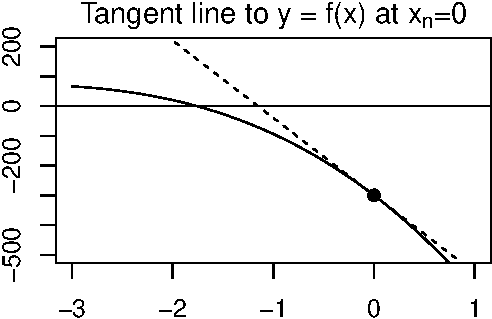
\includegraphics[keepaspectratio]{computation_files/figure-pdf/unnamed-chunk-1-1.pdf}}
\end{center}

The equation of the tangent line to the curve \(y = f(x)\) at a point
\(x = x_n\) is \[y = f'(x_n)(x-x_n) + f(x_n)\]

\begin{center}
\pandocbounded{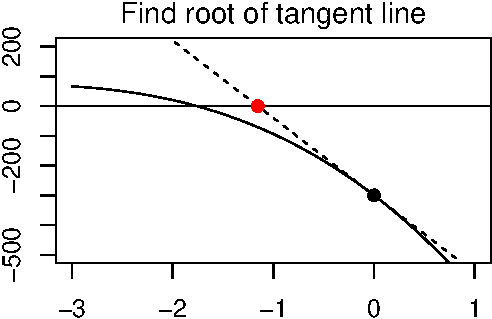
\includegraphics[keepaspectratio]{computation_files/figure-pdf/unnamed-chunk-2-1.pdf}}
\end{center}

The root of this tangent line (i.e., the place where it crosses the
x-axis) is easy to find:
\[0 = f'(x_n)(x-x_n) + f(x_n) \iff x = x_n - f(x_n)/f'(x_n)\]

Take this root of the tangent line as our next guess, then
repeat\ldots{}

\begin{center}
\pandocbounded{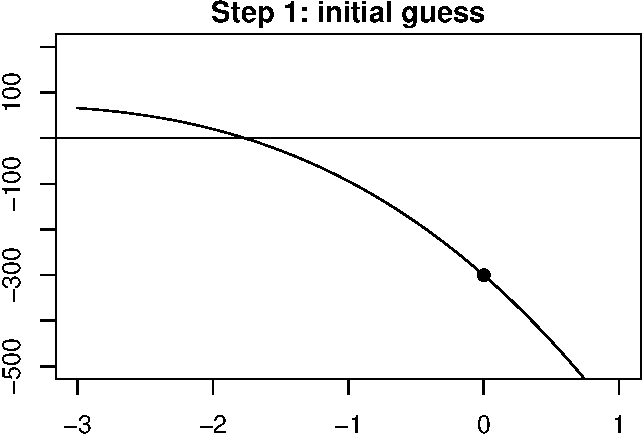
\includegraphics[keepaspectratio]{computation_files/figure-pdf/newton-step1-1.pdf}}
\end{center}

\ldots and repeat\ldots{}

\begin{center}
\pandocbounded{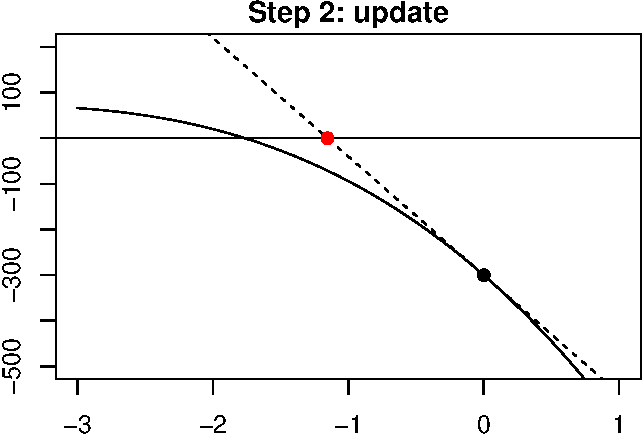
\includegraphics[keepaspectratio]{computation_files/figure-pdf/newton-step2-1.pdf}}
\end{center}

\ldots and repeat\ldots{}

\begin{center}
\pandocbounded{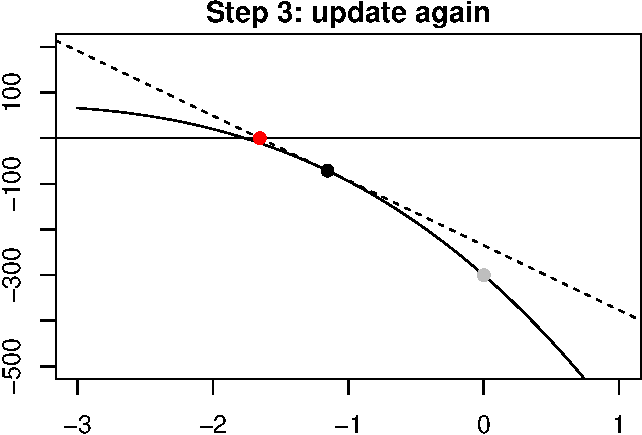
\includegraphics[keepaspectratio]{computation_files/figure-pdf/newton-step3-1.pdf}}
\end{center}

\ldots and repeat\ldots{}

\begin{center}
\pandocbounded{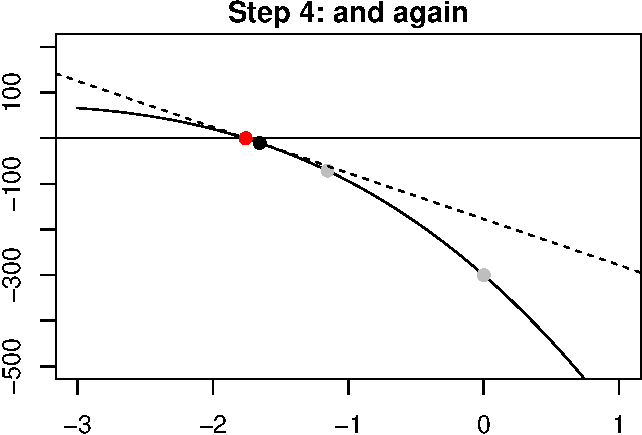
\includegraphics[keepaspectratio]{computation_files/figure-pdf/newton-step4-1.pdf}}
\end{center}

\ldots and repeat\ldots{}

\begin{center}
\pandocbounded{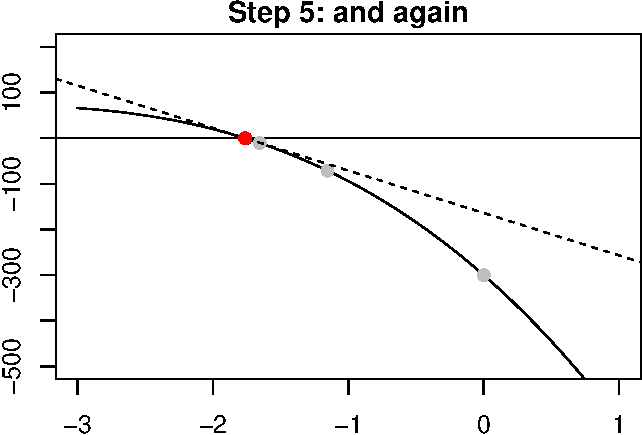
\includegraphics[keepaspectratio]{computation_files/figure-pdf/newton-step5-1.pdf}}
\end{center}

\ldots and keep repeating until you've converged!

The multivariate version of Newton-Raphson is called the
\href{https://en.wikipedia.org/wiki/Scoring_algorithm}{Scoring
algorithm} (also sometimes called Fisher's scoring), and is used in
\(\texttt{R}\) to obtain estimates of logistic regression coefficients.

\subsection*{Motivating Example: Logistic
Regression}\label{motivating-example-logistic-regression}

Suppose that we observe data \((y_i, x_i)\) where the outcome \(y\) is
binary. A natural model for these data is to assume the statistical
model

\begin{align*}
y_i & \sim Bernoulli(p_i), \\
\text{log} \left( \frac{p_i}{1 - p_i} \right) & = \beta_0 + \beta_1 x_i.
\end{align*}

This is a simple logistic regression model, with unknown parameters
given by the logistic regression coefficients \(\beta_0, \beta_1\).
Let's attempt to find MLEs for \(\beta_0\) and \(\beta_1\) analytically.

Note that
\(p_i = \frac{e^{\beta_0 + \beta_1 x_i}}{1 + e^{\beta_0 + \beta_1 x_i}}\).
Then the likelihood of our Bernoulli observations \(y_i\) can be written
as

\[
L(\beta_0, \beta_1) = \prod_{i = 1}^n \left( \frac{e^{\beta_0 + \beta_1 x_i}}{1 + e^{\beta_0 + \beta_1 x_i}} \right)^{y_i} \left( \frac{1}{1 + e^{\beta_0 + \beta_1 x_i}} \right)^{1 - y_i}
\]

Following the typical procedure, we log the likelihood\ldots{}

\begin{align*}
    \log(L(\beta_0, \beta_1)) & = \sum_{i = 1}^n \left[ y_i \log(\frac{e^{\beta_0 + \beta_1 x_i}}{1 + e^{\beta_0 + \beta_1 x_i}}) + (1 - y_i) \log(\frac{1}{1 + e^{\beta_0 + \beta_1 x_i}}) \right] \\
    & = \sum_{i = 1}^n \left[ y_i (\beta_0 + \beta_1 x_i) - y_i \log(1 + e^{\beta_0 + \beta_1 x_i}) - \log(1 + e^{\beta_0 + \beta_1 x_i}) + y_i \log(1 + e^{\beta_0 + \beta_1 x_i})\right] \\
    & = \sum_{i = 1}^n \left[ y_i (\beta_0 + \beta_1 x_i)  - \log(1 + e^{\beta_0 + \beta_1 x_i}) \right]
\end{align*}

\ldots taking the partial derivatives with respect to \(\beta_0\) and
\(\beta_1\) we get\ldots{}

\begin{align*}
    \frac{\partial}{\partial \beta_0} \log(L(\beta_0, \beta_1)) & = \sum_{i = 1}^n \left[ y_i -\frac{e^{\beta_0 + \beta_1 x_i}}{1 + e^{\beta_0 + \beta_1 x_i}}  \right]\\
    \frac{\partial}{\partial \beta_1} \log(L(\beta_0, \beta_1)) & = \sum_{i = 1}^n \left[ x_i \left( y_i -\frac{e^{\beta_0 + \beta_1 x_i}}{1 + e^{\beta_0 + \beta_1 x_i}} \right) \right]
\end{align*}

\ldots and if you try to solve the system of equations given by

\begin{align*}
    0 & \equiv \sum_{i = 1}^n \left[ y_i -\frac{e^{\beta_0 + \beta_1 x_i}}{1 + e^{\beta_0 + \beta_1 x_i}}  \right]\\
    0 & \equiv \sum_{i = 1}^n \left[ x_i \left( y_i -\frac{e^{\beta_0 + \beta_1 x_i}}{1 + e^{\beta_0 + \beta_1 x_i}} \right) \right]
\end{align*}

you'll get nowhere! There is no analytical (sometimes called
``closed-form'') solution. In this case, we'd need to use the Scoring
algorithm to solve for the regression coefficient estimates, since we
have more than one unknown parameter.

\subsection*{Why do anything analytically, if Newton-Raphson
exists?}\label{why-do-anything-analytically-if-newton-raphson-exists}

You may be wondering why you've been doing calculus/algebra the entire
semester, when such an algorithm exists. The answer is two-fold.

\begin{enumerate}
\def\labelenumi{\arabic{enumi}.}
\item
  Going through the steps of finding an MLE analytically helps build
  intuition. We saw that in the vast majority of cases, maximum
  likelihood estimators are functions of sample means. This is less
  obvious when doing everything numerically (using an algorithm). In
  addition to gaining insight from finding MLEs by hand, this practice
  also gave you the opportunity to learn/use common ``tricks'' in
  statistics, that will find their way into problems you complete down
  the road or research you may eventually conduct.
\item
  Numerical optimization is \emph{slow}. For simple cases like the ones
  we've seen in class, numerical optimization would techniques like
  Newton-Raphson would run relatively quickly. However, for more complex
  likelihoods with many unknown parameters, various optimization
  techniques can be so slow as to be computationally prohibitive. Even
  with continual improvements in computational power (and improvements
  in the algorithms themselves), computational speed is an important
  consideration when conducting statistical research or developing new
  methodology. If it takes someone two weeks to fit their regression
  model using numerical optimization, for example, that person may never
  fit a regression model ever again, or give up entirely. Especially
  when considering \emph{who} has access to computational power, this
  can become an equity issue. If you can solve something analytically,
  \textbf{do it}. It's significantly faster in the long-term, even it
  takes you some time to do the calculus/algebra.
\end{enumerate}

\section{Simulation Studies}\label{simulation-studies}

Sometimes proofs are hard. In such cases (and more generally), it can
often be useful to ``test'' or observe properties of estimators in a
computational setting, rather than in a rigorous mathematical context.
This is where simulation studies come into play, and if you eventually
find yourself conducting statistical research, knowing how to conduct a
well-designed, reproducible, simulation study is an incredibly important
skill.

The general idea of simulation study is to generate realistic settings
(data) that could be observed in the real world, in order to compare
properties of various estimators and their behavior in scenarios where
the ``truth'' is \emph{known} (because \emph{you} generated the truth!).
Steps include:

\begin{enumerate}
\def\labelenumi{\arabic{enumi}.}
\item
  Determine your simulation settings (different parameter values, sample
  sizes, etc.)
\item
  Generate \emph{many} data sets for each setting
\item
  Compute your estimator / implement your method for each data set
\item
  Record the relevant property of that estimator / method for each data
  set
\item
  Summarize your results across data sets and simulation settings
\end{enumerate}

This can be a \emph{great} way to get a feel for how certain
estimators/methods behave in different settings without needing to
rigorously prove something. Additionally, it can be used to
\emph{inform} more rigorous proofs down the line; if we can better
understand how estimators/methods behave, we may be able to relate that
behavior to existing proofs and build upon them!

\section{Gibbs Samplers}\label{gibbs-samplers}

Not everything is conjugate. In cases where we don't have conjugate
priors, posterior distributions may not have closed-form, analytical
pdfs, and instead we rely on Markov-chain Monte-Carlo (MCMC) algorithms
(or Laplace approximations) to generate samples from posteriors.

As noted in the Bayes chapter of our course notes,
\href{https://www.bayesrulesbook.com/}{Bayes Rules!} is a great place to
go for an introduction to Bayesian statistics. Here, we'll talk through
one (classical) example of an MCMC approach to posterior inference;
Gibbs Samplers.

The gist of Gibbs Sampling is that, when we have more than one unknown
parameter, we can obtain the \emph{joint} posterior distribution for all
parameters by updating our guesses about each parameter, one at a time.
This involves working with what are typically called \emph{full
conditionals} (the distribution of each parameter \emph{conditional on
everything else}).

The Gibbs Sampling algorithm is as follows:

\begin{enumerate}
\def\labelenumi{\arabic{enumi}.}
\item
  Choose initial values for each unknown parameter, \(\theta_1^{(0)}\),
  \(\theta_2^{(0)}\), \ldots, \(\theta_p^{(0)}\)
\item
  Sample
  \(\theta_{1}^{(0)} \sim \pi(\theta_{1}^{(0)} \mid \theta_{2}^{(0)}, \dots, \theta_{p}^{(0)},\textbf{y})\)
\item
  Sample
  \(\theta_{2}^{(0)} \sim \pi(\theta_{2}^{(0)} \mid, \theta_{1}^{(0)}, \theta_{3}^{(0)}, \dots, \theta_{p}^{(0)},\textbf{y})\)
\item
  \ldots{}
\item
  Sample
  \(\theta_{p}^{(0)} \sim \pi(\theta_{p}^{(0)} \mid \theta_{1}^{(0)}, \dots, \theta_{p-1}^{(0)},\textbf{y})\)
\item
  Repeat many times, always sampling new observations conditional on
  your most recent guess (iteration) for each parameter!
\end{enumerate}

It feels almost magical, but the end result is that we obtain many
samples from the joint posterior distribution for all unknown
parameters! MCMC methods such as Gibbs Samplers are what is known as
``exact'' methods for conducting Bayesian inference, because so long as
sampling goes according to plan*, the posterior draws will be from the
exactly correct, joint posterior distribution. This is opposed to
Laplace approximation techniques which are, by definition,
``approximate.''

*Let's define ``according to plan.'' Sometimes algorithms can go wrong.
We saw an example of this with Newton-Raphson, where if we pick a
terrible starting value, the algorithm can sometimes diverge. With Gibbs
Samplers, we should be careful of checking convergence diagnostics. A
visual tool for this is called a \textbf{Trace Plot}. Trace plots show
the values of parameters that are being sampled across iterations. The
values across iterations are referred to as \textbf{chains}.

Here are some examples of chains that have converged:

\pandocbounded{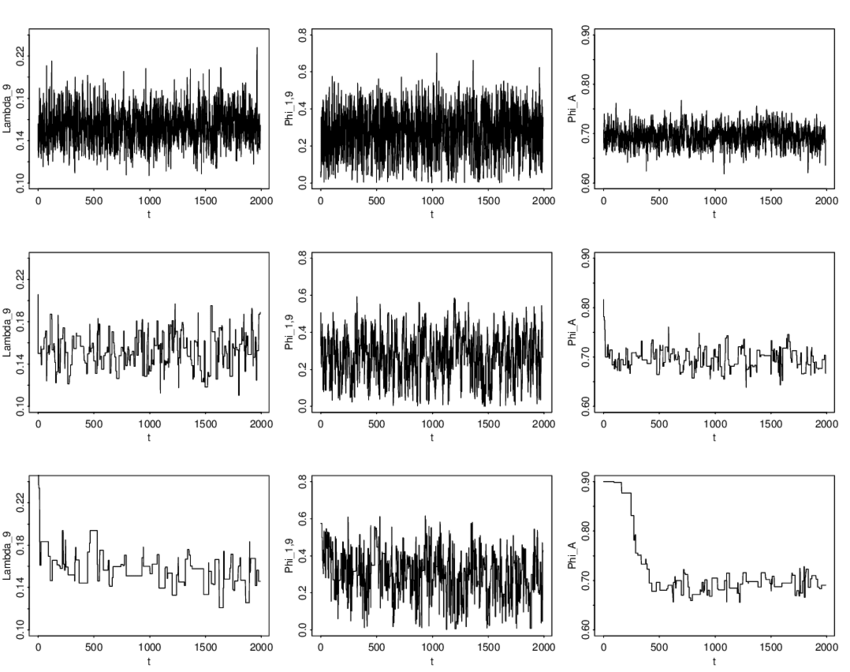
\includegraphics[keepaspectratio]{images/traceplots.png}}

There are \emph{many} other convergence diagnostics you will need to
consider if you end up doing research involving MCMC algorithms. A
recent research paper on convergence diagnostics that is generally
accepted now as best practice among Bayesian statisticians can be found
\href{https://arxiv.org/pdf/1903.08008.pdf}{here}.




\end{document}
